\PassOptionsToPackage{unicode=true}{hyperref} % options for packages loaded elsewhere
\PassOptionsToPackage{hyphens}{url}
%
\documentclass[]{book}
\usepackage{lmodern}
\usepackage{amssymb,amsmath}
\usepackage{ifxetex,ifluatex}
\usepackage{fixltx2e} % provides \textsubscript
\ifnum 0\ifxetex 1\fi\ifluatex 1\fi=0 % if pdftex
  \usepackage[T1]{fontenc}
  \usepackage[utf8]{inputenc}
  \usepackage{textcomp} % provides euro and other symbols
\else % if luatex or xelatex
  \usepackage{unicode-math}
  \defaultfontfeatures{Ligatures=TeX,Scale=MatchLowercase}
\fi
% use upquote if available, for straight quotes in verbatim environments
\IfFileExists{upquote.sty}{\usepackage{upquote}}{}
% use microtype if available
\IfFileExists{microtype.sty}{%
\usepackage[]{microtype}
\UseMicrotypeSet[protrusion]{basicmath} % disable protrusion for tt fonts
}{}
\IfFileExists{parskip.sty}{%
\usepackage{parskip}
}{% else
\setlength{\parindent}{0pt}
\setlength{\parskip}{6pt plus 2pt minus 1pt}
}
\usepackage{hyperref}
\hypersetup{
            pdftitle={Tutoriel : visualisation avec R},
            pdfauthor={Laurent Rouvière},
            pdfborder={0 0 0},
            breaklinks=true}
\urlstyle{same}  % don't use monospace font for urls
\usepackage{color}
\usepackage{fancyvrb}
\newcommand{\VerbBar}{|}
\newcommand{\VERB}{\Verb[commandchars=\\\{\}]}
\DefineVerbatimEnvironment{Highlighting}{Verbatim}{commandchars=\\\{\}}
% Add ',fontsize=\small' for more characters per line
\usepackage{framed}
\definecolor{shadecolor}{RGB}{248,248,248}
\newenvironment{Shaded}{\begin{snugshade}}{\end{snugshade}}
\newcommand{\AlertTok}[1]{\textcolor[rgb]{0.94,0.16,0.16}{#1}}
\newcommand{\AnnotationTok}[1]{\textcolor[rgb]{0.56,0.35,0.01}{\textbf{\textit{#1}}}}
\newcommand{\AttributeTok}[1]{\textcolor[rgb]{0.77,0.63,0.00}{#1}}
\newcommand{\BaseNTok}[1]{\textcolor[rgb]{0.00,0.00,0.81}{#1}}
\newcommand{\BuiltInTok}[1]{#1}
\newcommand{\CharTok}[1]{\textcolor[rgb]{0.31,0.60,0.02}{#1}}
\newcommand{\CommentTok}[1]{\textcolor[rgb]{0.56,0.35,0.01}{\textit{#1}}}
\newcommand{\CommentVarTok}[1]{\textcolor[rgb]{0.56,0.35,0.01}{\textbf{\textit{#1}}}}
\newcommand{\ConstantTok}[1]{\textcolor[rgb]{0.00,0.00,0.00}{#1}}
\newcommand{\ControlFlowTok}[1]{\textcolor[rgb]{0.13,0.29,0.53}{\textbf{#1}}}
\newcommand{\DataTypeTok}[1]{\textcolor[rgb]{0.13,0.29,0.53}{#1}}
\newcommand{\DecValTok}[1]{\textcolor[rgb]{0.00,0.00,0.81}{#1}}
\newcommand{\DocumentationTok}[1]{\textcolor[rgb]{0.56,0.35,0.01}{\textbf{\textit{#1}}}}
\newcommand{\ErrorTok}[1]{\textcolor[rgb]{0.64,0.00,0.00}{\textbf{#1}}}
\newcommand{\ExtensionTok}[1]{#1}
\newcommand{\FloatTok}[1]{\textcolor[rgb]{0.00,0.00,0.81}{#1}}
\newcommand{\FunctionTok}[1]{\textcolor[rgb]{0.00,0.00,0.00}{#1}}
\newcommand{\ImportTok}[1]{#1}
\newcommand{\InformationTok}[1]{\textcolor[rgb]{0.56,0.35,0.01}{\textbf{\textit{#1}}}}
\newcommand{\KeywordTok}[1]{\textcolor[rgb]{0.13,0.29,0.53}{\textbf{#1}}}
\newcommand{\NormalTok}[1]{#1}
\newcommand{\OperatorTok}[1]{\textcolor[rgb]{0.81,0.36,0.00}{\textbf{#1}}}
\newcommand{\OtherTok}[1]{\textcolor[rgb]{0.56,0.35,0.01}{#1}}
\newcommand{\PreprocessorTok}[1]{\textcolor[rgb]{0.56,0.35,0.01}{\textit{#1}}}
\newcommand{\RegionMarkerTok}[1]{#1}
\newcommand{\SpecialCharTok}[1]{\textcolor[rgb]{0.00,0.00,0.00}{#1}}
\newcommand{\SpecialStringTok}[1]{\textcolor[rgb]{0.31,0.60,0.02}{#1}}
\newcommand{\StringTok}[1]{\textcolor[rgb]{0.31,0.60,0.02}{#1}}
\newcommand{\VariableTok}[1]{\textcolor[rgb]{0.00,0.00,0.00}{#1}}
\newcommand{\VerbatimStringTok}[1]{\textcolor[rgb]{0.31,0.60,0.02}{#1}}
\newcommand{\WarningTok}[1]{\textcolor[rgb]{0.56,0.35,0.01}{\textbf{\textit{#1}}}}
\usepackage{longtable,booktabs}
% Fix footnotes in tables (requires footnote package)
\IfFileExists{footnote.sty}{\usepackage{footnote}\makesavenoteenv{longtable}}{}
\usepackage{graphicx,grffile}
\makeatletter
\def\maxwidth{\ifdim\Gin@nat@width>\linewidth\linewidth\else\Gin@nat@width\fi}
\def\maxheight{\ifdim\Gin@nat@height>\textheight\textheight\else\Gin@nat@height\fi}
\makeatother
% Scale images if necessary, so that they will not overflow the page
% margins by default, and it is still possible to overwrite the defaults
% using explicit options in \includegraphics[width, height, ...]{}
\setkeys{Gin}{width=\maxwidth,height=\maxheight,keepaspectratio}
\setlength{\emergencystretch}{3em}  % prevent overfull lines
\providecommand{\tightlist}{%
  \setlength{\itemsep}{0pt}\setlength{\parskip}{0pt}}
\setcounter{secnumdepth}{5}
% Redefines (sub)paragraphs to behave more like sections
\ifx\paragraph\undefined\else
\let\oldparagraph\paragraph
\renewcommand{\paragraph}[1]{\oldparagraph{#1}\mbox{}}
\fi
\ifx\subparagraph\undefined\else
\let\oldsubparagraph\subparagraph
\renewcommand{\subparagraph}[1]{\oldsubparagraph{#1}\mbox{}}
\fi

% set default figure placement to htbp
\makeatletter
\def\fps@figure{htbp}
\makeatother

\usepackage{booktabs}
\usepackage[]{natbib}
\bibliographystyle{apalike}

\title{Tutoriel : visualisation avec R}
\author{Laurent Rouvière}
\date{2020-05-29}

\usepackage{amsthm}
\newtheorem{theorem}{Theorem}[chapter]
\newtheorem{lemma}{Lemma}[chapter]
\newtheorem{corollary}{Corollary}[chapter]
\newtheorem{proposition}{Proposition}[chapter]
\newtheorem{conjecture}{Conjecture}[chapter]
\theoremstyle{definition}
\newtheorem{definition}{Definition}[chapter]
\theoremstyle{definition}
\newtheorem{example}{Example}[chapter]
\theoremstyle{definition}
\newtheorem{exercise}{Exercice}[chapter]
\theoremstyle{remark}
\newtheorem*{remark}{Remark}
\newtheorem*{solution}{Solution}
\let\BeginKnitrBlock\begin \let\EndKnitrBlock\end
\begin{document}
\maketitle

{
\setcounter{tocdepth}{1}
\tableofcontents
}
\hypertarget{Presentation}{%
\chapter*{Présentation}\label{Presentation}}
\addcontentsline{toc}{chapter}{Présentation}

Ce tutoriel présente quelques outils \textbf{R} pour la \textbf{visualisation de données}. Il nécessite des connaissance de base en \textbf{R} et en programmation et se structure en 3 parties :

\begin{itemize}
\tightlist
\item
  \texttt{Visualisation\ avec\ ggplot2} : présentation du package \textbf{ggplot2} pour faire des représentations graphiques avec \textbf{R} ;
\item
  \texttt{Introduction\ à\ la\ cartographie} : construction de cartes avec les packages \texttt{ggmap}, \texttt{sf} et \texttt{leaflet} ;
\item
  \texttt{Visualisation\ interactive}: présentation de packages qui permettent de faire facilement des graphes interactifs, des tableaux de bord ou des applications web (\textbf{shiny}).
\end{itemize}

On pourra trouver des transparents associés à ce tutoriel ainsi que les données utilisés à l'adresse suivante \url{https://lrouviere.github.io/VISU/}.

\hypertarget{ggplot2}{%
\chapter{Visualisation avec ggplot2}\label{ggplot2}}

Il est souvent nécessaire d'utiliser des techniques de visualisation à toutes les étapes d'une étude statistique. Un des avantages de \textbf{R} est qu'il est relativement simple de mettre en oeuvre tout les types de graphes généralement utilisés. Dans cette fiche, nous présentons tout d'abord les fonctions classiques qui permettent de tracer des figures. Nous proposons ensuite une introduction aux graphes \textbf{ggplot} qui sont de plus en plus utilisés pour faire de la visualisation.

\hypertarget{fonctions-graphiques-conventionnelles}{%
\section{Fonctions graphiques conventionnelles}\label{fonctions-graphiques-conventionnelles}}

Pour commencer il est intéressant d'examiner quelques exemples de représentations graphiques construits avec \textbf{R}. On peut les obtenir à l'aide de la fonction \textbf{demo}.

\begin{Shaded}
\begin{Highlighting}[]
\OperatorTok{>}\StringTok{ }\KeywordTok{demo}\NormalTok{(graphics)}
\end{Highlighting}
\end{Shaded}

\hypertarget{la-fonction-plot}{%
\subsection{\texorpdfstring{La fonction \textbf{plot}}{La fonction plot}}\label{la-fonction-plot}}

C'est une \textbf{fonction générique} que l'on peut utiliser pour représenter différents types de données. L'utilisation standard consiste à visualiser une variable \emph{y} en fonction d'une variable \emph{x}. On peut par exemple obtenir le graphe de la fonction \(x\mapsto \sin(2\pi x)\) sur \([0,1]\), à l'aide de

\begin{Shaded}
\begin{Highlighting}[]
\OperatorTok{>}\StringTok{ }\NormalTok{x <-}\StringTok{ }\KeywordTok{seq}\NormalTok{(}\OperatorTok{-}\DecValTok{2}\OperatorTok{*}\NormalTok{pi,}\DecValTok{2}\OperatorTok{*}\NormalTok{pi,}\DataTypeTok{by=}\FloatTok{0.05}\NormalTok{)}
\OperatorTok{>}\StringTok{ }\NormalTok{y <-}\StringTok{ }\KeywordTok{sin}\NormalTok{(x)}
\OperatorTok{>}\StringTok{ }\KeywordTok{plot}\NormalTok{(x,y) }\CommentTok{#points (par défaut)}
\end{Highlighting}
\end{Shaded}

\begin{center}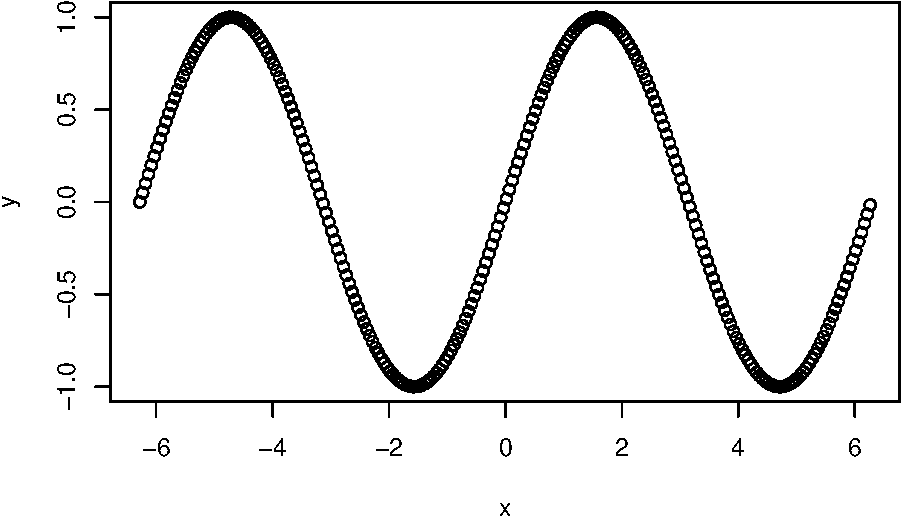
\includegraphics{TUTO_VISU_files/figure-latex/unnamed-chunk-4-1} \end{center}

\begin{Shaded}
\begin{Highlighting}[]
\OperatorTok{>}\StringTok{ }\KeywordTok{plot}\NormalTok{(x,y,}\DataTypeTok{type=}\StringTok{"l"}\NormalTok{) }\CommentTok{#représentation sous forme de ligne}
\end{Highlighting}
\end{Shaded}

\begin{center}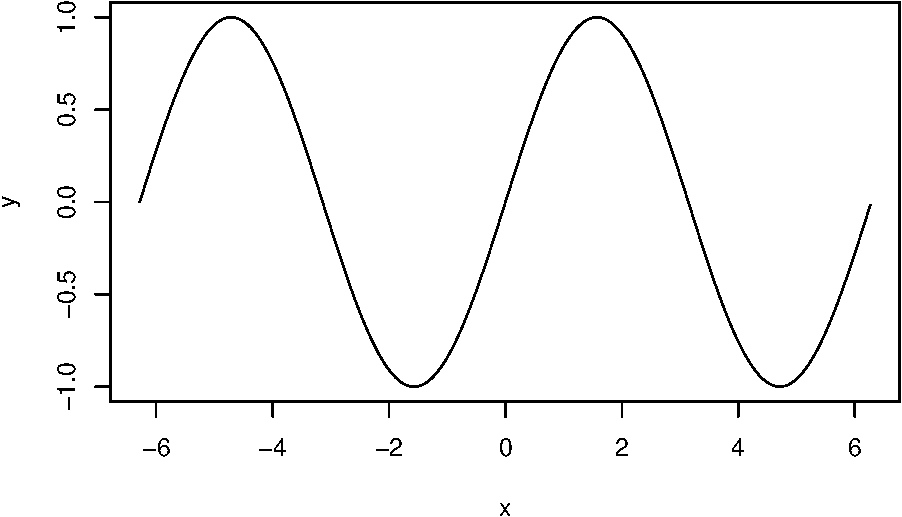
\includegraphics{TUTO_VISU_files/figure-latex/unnamed-chunk-4-2} \end{center}

Nous proposons des exemples de représentations de variables quantitatives et qualitatives à l'aide du jeu de données \textbf{ozone.txt} que l'on importe avec

\begin{Shaded}
\begin{Highlighting}[]
\OperatorTok{>}\StringTok{ }\NormalTok{ozone <-}\StringTok{ }\KeywordTok{read.table}\NormalTok{(}\StringTok{"ozone.txt"}\NormalTok{)}
\OperatorTok{>}\StringTok{ }\KeywordTok{summary}\NormalTok{(ozone)}
\CommentTok{##      maxO3              T9             T12             T15       }
\CommentTok{##  Min.   : 42.00   Min.   :11.30   Min.   :14.00   Min.   :14.90  }
\CommentTok{##  1st Qu.: 70.75   1st Qu.:16.20   1st Qu.:18.60   1st Qu.:19.27  }
\CommentTok{##  Median : 81.50   Median :17.80   Median :20.55   Median :22.05  }
\CommentTok{##  Mean   : 90.30   Mean   :18.36   Mean   :21.53   Mean   :22.63  }
\CommentTok{##  3rd Qu.:106.00   3rd Qu.:19.93   3rd Qu.:23.55   3rd Qu.:25.40  }
\CommentTok{##  Max.   :166.00   Max.   :27.00   Max.   :33.50   Max.   :35.50  }
\CommentTok{##       Ne9             Ne12            Ne15           Vx9         }
\CommentTok{##  Min.   :0.000   Min.   :0.000   Min.   :0.00   Min.   :-7.8785  }
\CommentTok{##  1st Qu.:3.000   1st Qu.:4.000   1st Qu.:3.00   1st Qu.:-3.2765  }
\CommentTok{##  Median :6.000   Median :5.000   Median :5.00   Median :-0.8660  }
\CommentTok{##  Mean   :4.929   Mean   :5.018   Mean   :4.83   Mean   :-1.2143  }
\CommentTok{##  3rd Qu.:7.000   3rd Qu.:7.000   3rd Qu.:7.00   3rd Qu.: 0.6946  }
\CommentTok{##  Max.   :8.000   Max.   :8.000   Max.   :8.00   Max.   : 5.1962  }
\CommentTok{##       Vx12             Vx15            maxO3v          vent      pluie   }
\CommentTok{##  Min.   :-7.878   Min.   :-9.000   Min.   : 42.00   Est  :10   Pluie:43  }
\CommentTok{##  1st Qu.:-3.565   1st Qu.:-3.939   1st Qu.: 71.00   Nord :31   Sec  :69  }
\CommentTok{##  Median :-1.879   Median :-1.550   Median : 82.50   Ouest:50             }
\CommentTok{##  Mean   :-1.611   Mean   :-1.691   Mean   : 90.57   Sud  :21             }
\CommentTok{##  3rd Qu.: 0.000   3rd Qu.: 0.000   3rd Qu.:106.00                        }
\CommentTok{##  Max.   : 6.578   Max.   : 5.000   Max.   :166.00}
\end{Highlighting}
\end{Shaded}

On visualise tout d'abord 2 variables quantitatives à l'aide d'un nuage de points : la concentration en ozone maximale \textbf{maxO3} en fonction de la température à 12h \textbf{T12}.

\begin{Shaded}
\begin{Highlighting}[]
\OperatorTok{>}\StringTok{ }\KeywordTok{plot}\NormalTok{(ozone[,}\StringTok{"T12"}\NormalTok{],ozone[,}\StringTok{"maxO3"}\NormalTok{])}
\end{Highlighting}
\end{Shaded}

\begin{center}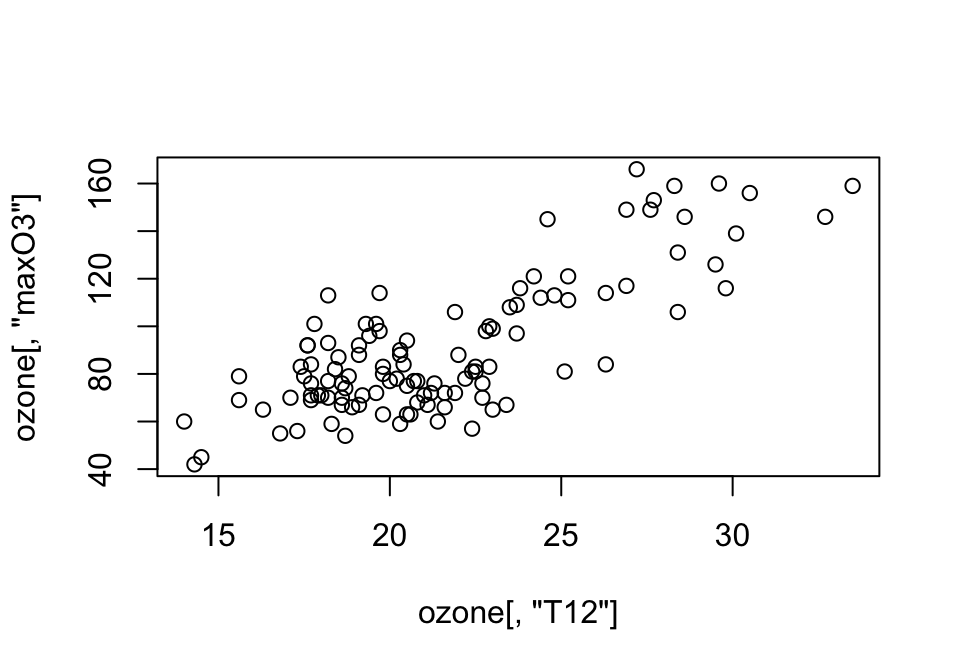
\includegraphics{TUTO_VISU_files/figure-latex/unnamed-chunk-6-1} \end{center}

Comme les deux variables appartiennent au même jeu de données, on peut obtenir la même représentation à l'aide d'une sytaxe plus claire qui ajoutent automatiquement les noms des variables sur les axes :

\begin{Shaded}
\begin{Highlighting}[]
\OperatorTok{>}\StringTok{ }\KeywordTok{plot}\NormalTok{(maxO3}\OperatorTok{~}\NormalTok{T12,}\DataTypeTok{data=}\NormalTok{ozone)}
\end{Highlighting}
\end{Shaded}

\begin{center}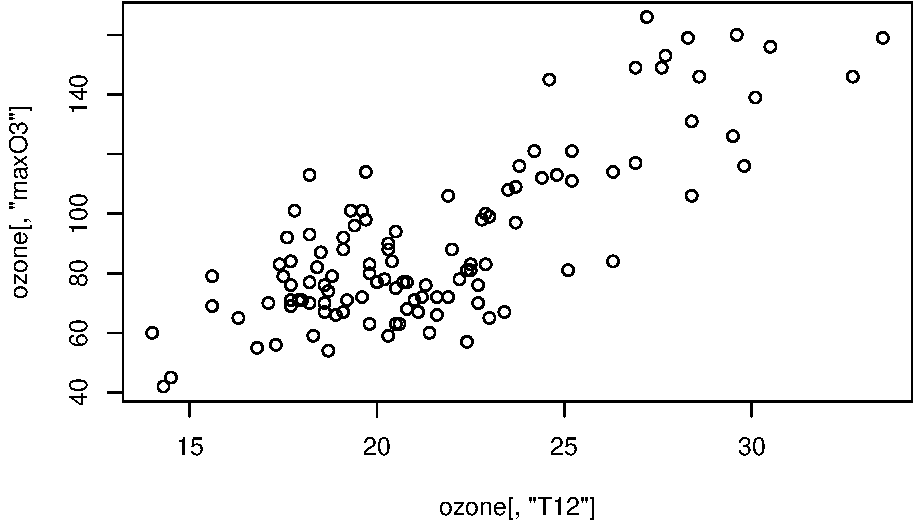
\includegraphics{TUTO_VISU_files/figure-latex/unnamed-chunk-7-1} \end{center}

Une autre façon de faire (moins naturelle) :

\begin{Shaded}
\begin{Highlighting}[]
\OperatorTok{>}\StringTok{ }\KeywordTok{plot}\NormalTok{(ozone[,}\StringTok{"T12"}\NormalTok{],ozone[,}\StringTok{"maxO3"}\NormalTok{],}\DataTypeTok{xlab=}\StringTok{"T12"}\NormalTok{,}\DataTypeTok{ylab=}\StringTok{"maxO3"}\NormalTok{)}
\end{Highlighting}
\end{Shaded}

\begin{center}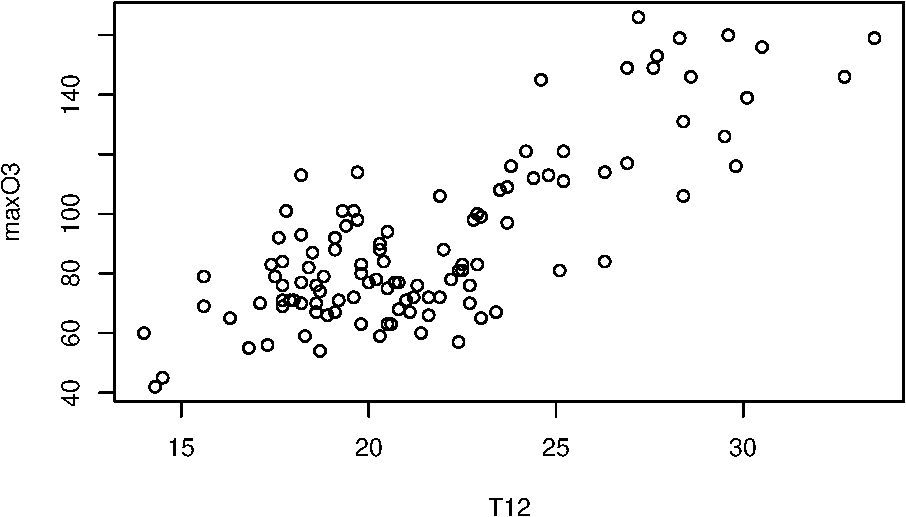
\includegraphics{TUTO_VISU_files/figure-latex/unnamed-chunk-8-1} \end{center}

Il existe des fonctions spécifiques pour chaque type de graphs, par exemple \textbf{histogram}, \textbf{barplot} et \textbf{boxplot} :

\begin{Shaded}
\begin{Highlighting}[]
\OperatorTok{>}\StringTok{ }\KeywordTok{hist}\NormalTok{(ozone}\OperatorTok{$}\NormalTok{maxO3,}\DataTypeTok{main=}\StringTok{"Histogram"}\NormalTok{)}
\end{Highlighting}
\end{Shaded}

\begin{center}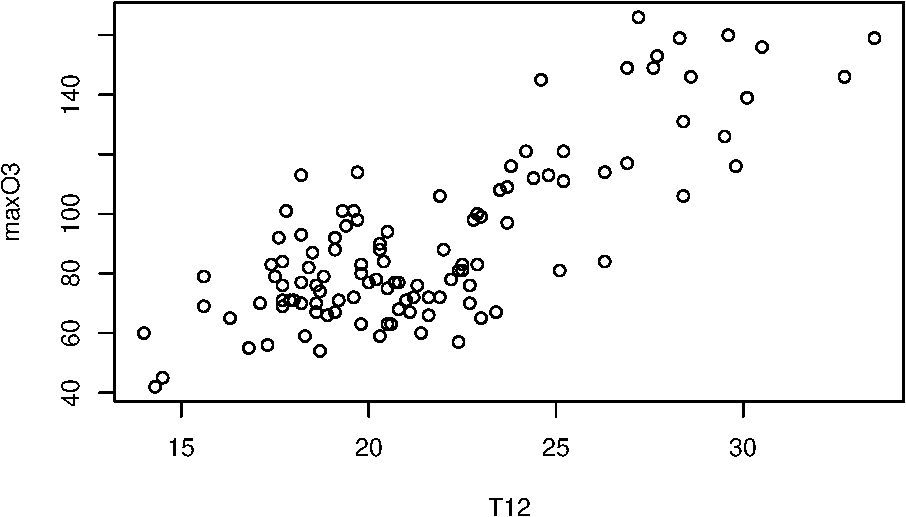
\includegraphics{TUTO_VISU_files/figure-latex/unnamed-chunk-9-1} \end{center}

\begin{Shaded}
\begin{Highlighting}[]
\OperatorTok{>}\StringTok{ }\KeywordTok{barplot}\NormalTok{(}\KeywordTok{table}\NormalTok{(ozone}\OperatorTok{$}\NormalTok{vent)}\OperatorTok{/}\KeywordTok{nrow}\NormalTok{(ozone),}\DataTypeTok{col=}\StringTok{"blue"}\NormalTok{)}
\end{Highlighting}
\end{Shaded}

\begin{center}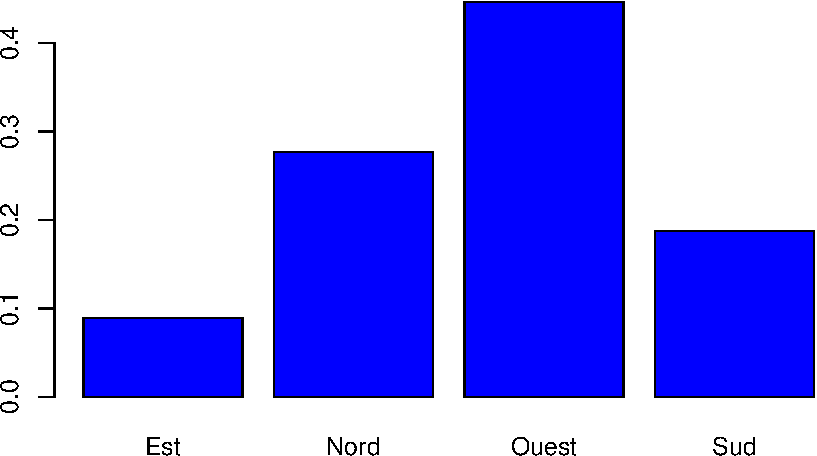
\includegraphics{TUTO_VISU_files/figure-latex/unnamed-chunk-9-2} \end{center}

\begin{Shaded}
\begin{Highlighting}[]
\OperatorTok{>}\StringTok{ }\KeywordTok{boxplot}\NormalTok{(maxO3}\OperatorTok{~}\NormalTok{vent,}\DataTypeTok{data=}\NormalTok{ozone)}
\end{Highlighting}
\end{Shaded}

\begin{center}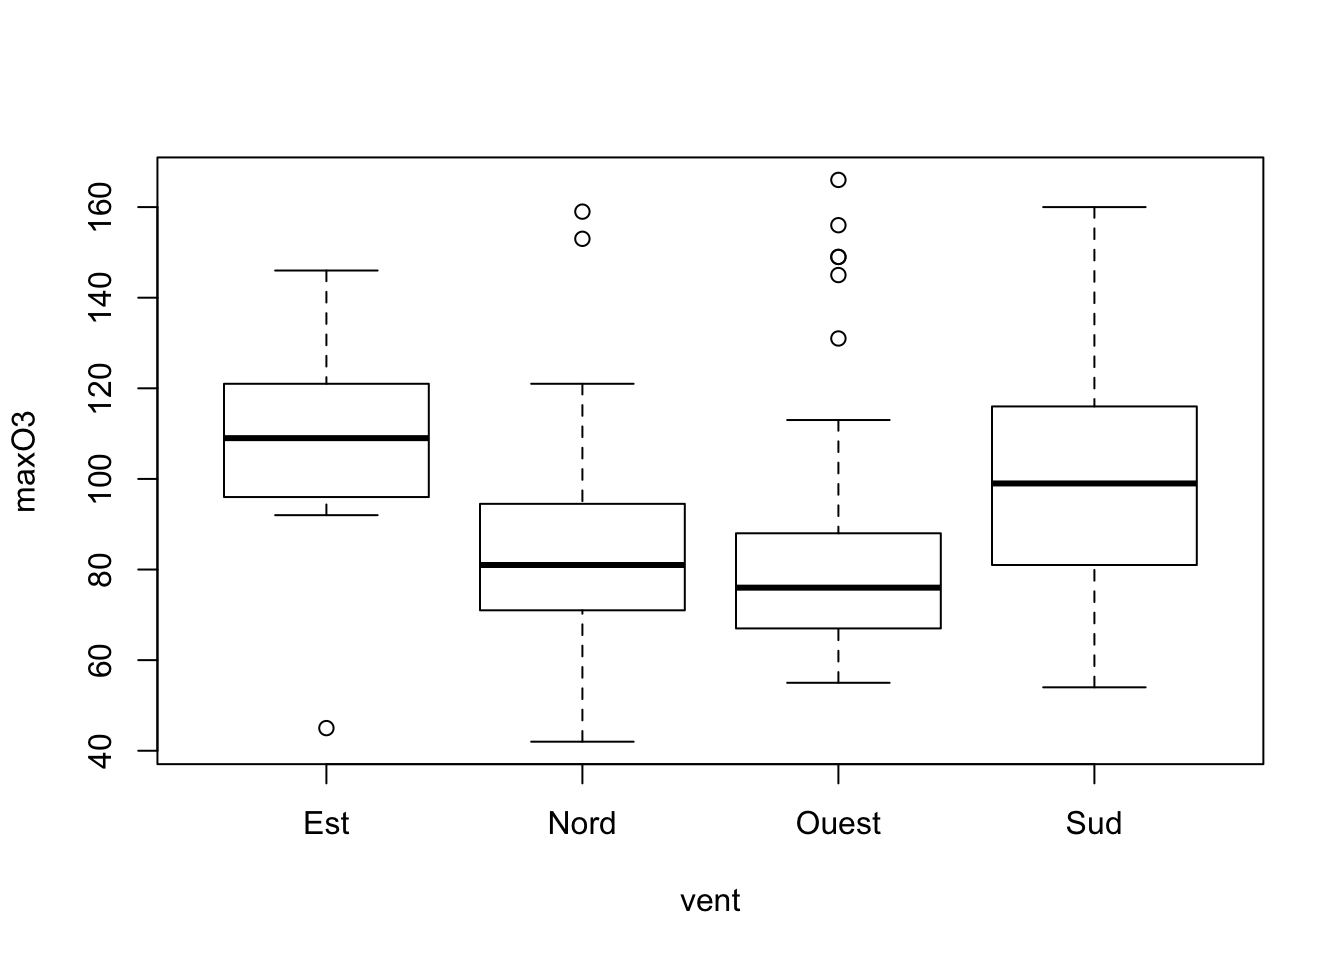
\includegraphics{TUTO_VISU_files/figure-latex/unnamed-chunk-9-3} \end{center}

\hypertarget{graphes-interactifs-avec-ramcharts}{%
\subsection{Graphes interactifs avec rAmCharts}\label{graphes-interactifs-avec-ramcharts}}

On peut utiliser ce package pour obtenir des graphes dynamiques. L'utilisation est relativement simple, il suffit d'ajouter le prefixe \textbf{am} devant le nom de la fonction :

\begin{Shaded}
\begin{Highlighting}[]
\OperatorTok{>}\StringTok{ }\KeywordTok{library}\NormalTok{(rAmCharts)}
\OperatorTok{>}\StringTok{ }\KeywordTok{amHist}\NormalTok{(ozone}\OperatorTok{$}\NormalTok{maxO3)}
\end{Highlighting}
\end{Shaded}

\begin{center}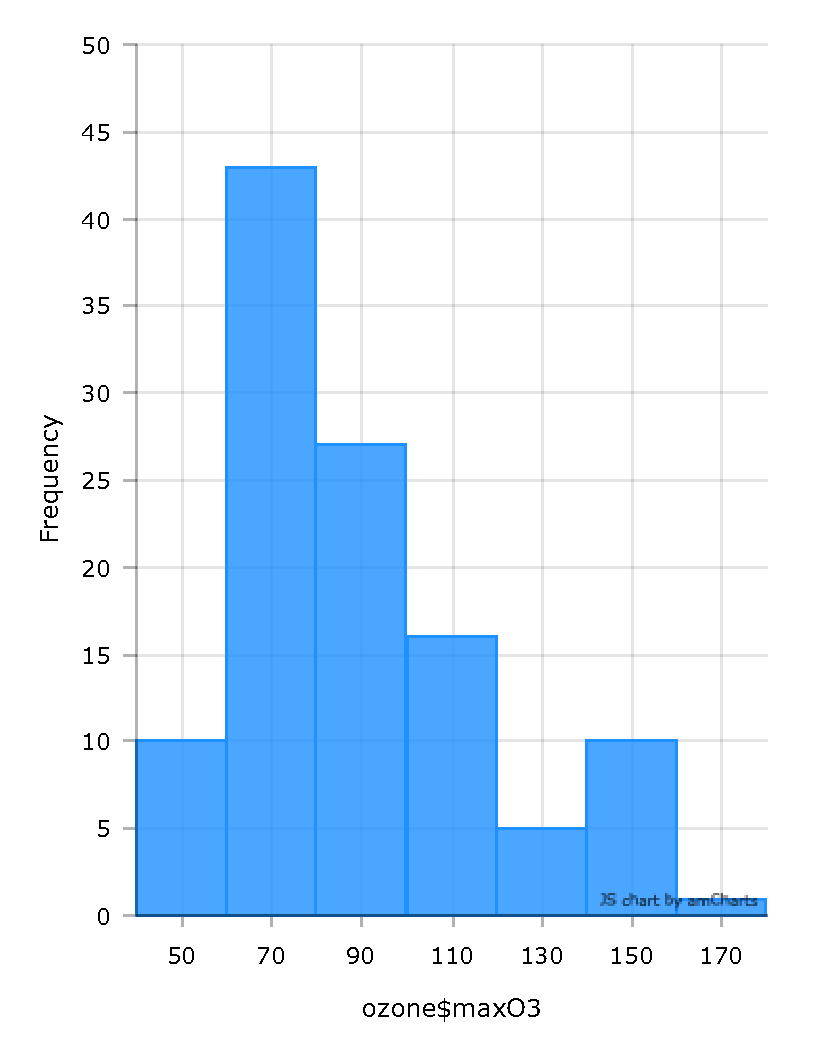
\includegraphics{TUTO_VISU_files/figure-latex/unnamed-chunk-10-1} \end{center}

\begin{Shaded}
\begin{Highlighting}[]
\OperatorTok{>}\StringTok{ }\KeywordTok{amPlot}\NormalTok{(ozone,}\DataTypeTok{col=}\KeywordTok{c}\NormalTok{(}\StringTok{"T9"}\NormalTok{,}\StringTok{"T12"}\NormalTok{))}
\end{Highlighting}
\end{Shaded}

\begin{center}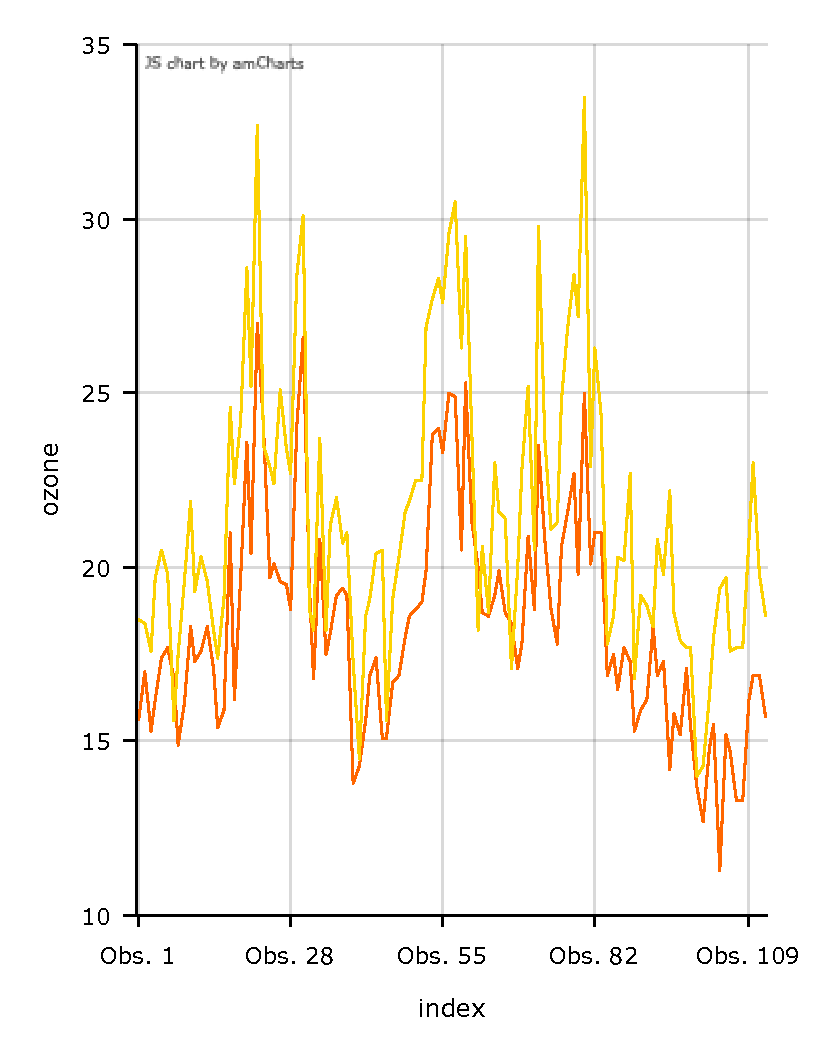
\includegraphics{TUTO_VISU_files/figure-latex/unnamed-chunk-10-2} \end{center}

\begin{Shaded}
\begin{Highlighting}[]
\OperatorTok{>}\StringTok{ }\KeywordTok{amBoxplot}\NormalTok{(maxO3}\OperatorTok{~}\NormalTok{vent,}\DataTypeTok{data=}\NormalTok{ozone)}
\end{Highlighting}
\end{Shaded}

\begin{center}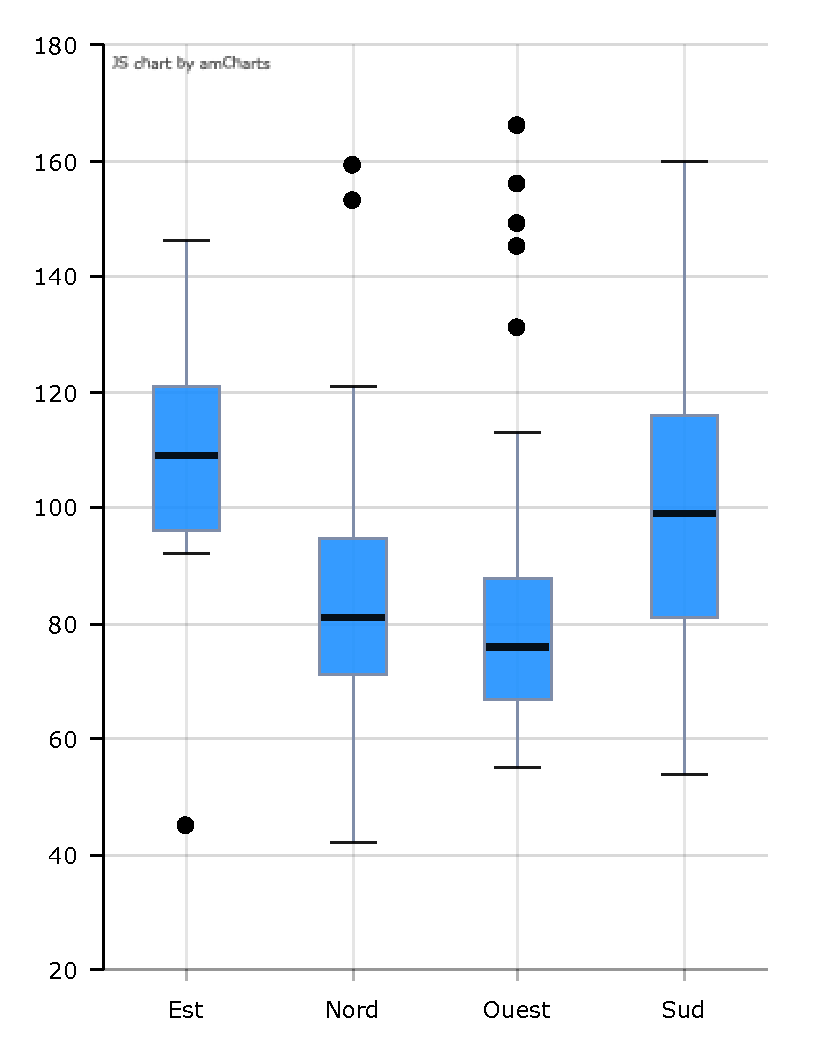
\includegraphics{TUTO_VISU_files/figure-latex/unnamed-chunk-10-3} \end{center}

\BeginKnitrBlock{exercise}[Premier graphe]
\protect\hypertarget{exr:exo1}{}{\label{exr:exo1} \iffalse (Premier graphe) \fi{} }
\EndKnitrBlock{exercise}

\begin{enumerate}
\def\labelenumi{\arabic{enumi}.}
\tightlist
\item
  Tracer la fonction \textbf{sinus} entre \(0\) et \(2\pi\).
\item
  A l'aide de la fonction \textbf{title} ajouter le titre \textbf{Représentation de la fonction sinus}.
\end{enumerate}

\begin{Shaded}
\begin{Highlighting}[]
\OperatorTok{>}\StringTok{ }\NormalTok{x <-}\StringTok{ }\KeywordTok{seq}\NormalTok{(}\DecValTok{0}\NormalTok{,}\DecValTok{2}\OperatorTok{*}\NormalTok{pi,}\DataTypeTok{length=}\DecValTok{1000}\NormalTok{)}
\OperatorTok{>}\StringTok{ }\KeywordTok{plot}\NormalTok{(x,}\KeywordTok{sin}\NormalTok{(x),}\DataTypeTok{type=}\StringTok{"l"}\NormalTok{)}
\OperatorTok{>}\StringTok{ }\KeywordTok{title}\NormalTok{(}\StringTok{"Représentation de la fonction sinus"}\NormalTok{)}
\end{Highlighting}
\end{Shaded}

\begin{center}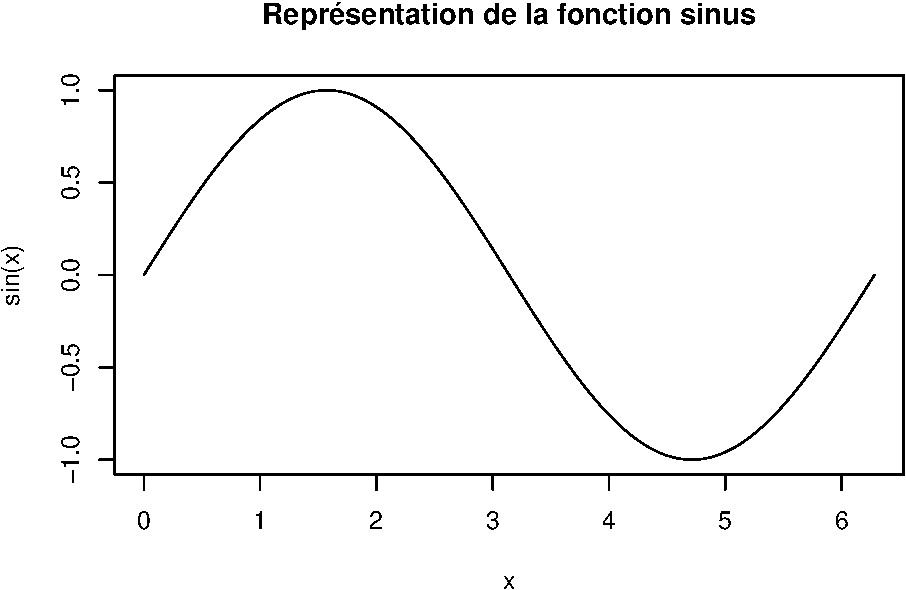
\includegraphics{TUTO_VISU_files/figure-latex/test-a-1} \end{center}

\BeginKnitrBlock{exercise}[Tracé de densités]
\protect\hypertarget{exr:exo2}{}{\label{exr:exo2} \iffalse (Tracé de densités) \fi{} }
\EndKnitrBlock{exercise}

\begin{enumerate}
\def\labelenumi{\arabic{enumi}.}
\tightlist
\item
  Tracer la densité de la loi normale centrée réduite entre \(-4\) et 4 (utiliser \textbf{dnorm}).
\item
  Ajouter une ligne verticale (en tirets) qui passe par \(x=0\) (utiliser \textbf{abline} avec \textbf{lty=2}).
\item
  Sur le même graphe, ajouter les densités de loi la de Student à 5 et 30 degrés de liberté (utiliser \textbf{dt}). On utilisera la fonction \textbf{lines} et des couleurs différentes pour chaque densité.
\item
  Ajouter une légende qui permet de repérer chaque densité (fonction \textbf{legend}).
\end{enumerate}

\begin{Shaded}
\begin{Highlighting}[]
\OperatorTok{>}\StringTok{ }\NormalTok{x <-}\StringTok{ }\KeywordTok{seq}\NormalTok{(}\OperatorTok{-}\DecValTok{4}\NormalTok{,}\DecValTok{4}\NormalTok{,}\DataTypeTok{by=}\FloatTok{0.01}\NormalTok{)}
\OperatorTok{>}\StringTok{ }\KeywordTok{plot}\NormalTok{(x,}\KeywordTok{dnorm}\NormalTok{(x),}\DataTypeTok{type=}\StringTok{"l"}\NormalTok{)}
\OperatorTok{>}\StringTok{ }\KeywordTok{abline}\NormalTok{(}\DataTypeTok{v=}\DecValTok{0}\NormalTok{,}\DataTypeTok{lty=}\DecValTok{2}\NormalTok{)}
\OperatorTok{>}\StringTok{ }\KeywordTok{lines}\NormalTok{(x,}\KeywordTok{dt}\NormalTok{(x,}\DecValTok{5}\NormalTok{),}\DataTypeTok{col=}\DecValTok{2}\NormalTok{)}
\OperatorTok{>}\StringTok{ }\KeywordTok{lines}\NormalTok{(x,}\KeywordTok{dt}\NormalTok{(x,}\DecValTok{30}\NormalTok{),}\DataTypeTok{col=}\DecValTok{3}\NormalTok{)}
\OperatorTok{>}\StringTok{ }\KeywordTok{legend}\NormalTok{(}\StringTok{"topleft"}\NormalTok{,}\DataTypeTok{legend=}\KeywordTok{c}\NormalTok{(}\StringTok{"normal"}\NormalTok{,}\StringTok{"Student(5)"}\NormalTok{,}\StringTok{"Student(30)"}\NormalTok{),}
\OperatorTok{+}\StringTok{        }\DataTypeTok{col=}\DecValTok{1}\OperatorTok{:}\DecValTok{3}\NormalTok{,}\DataTypeTok{lty=}\DecValTok{1}\NormalTok{)}
\end{Highlighting}
\end{Shaded}

\begin{center}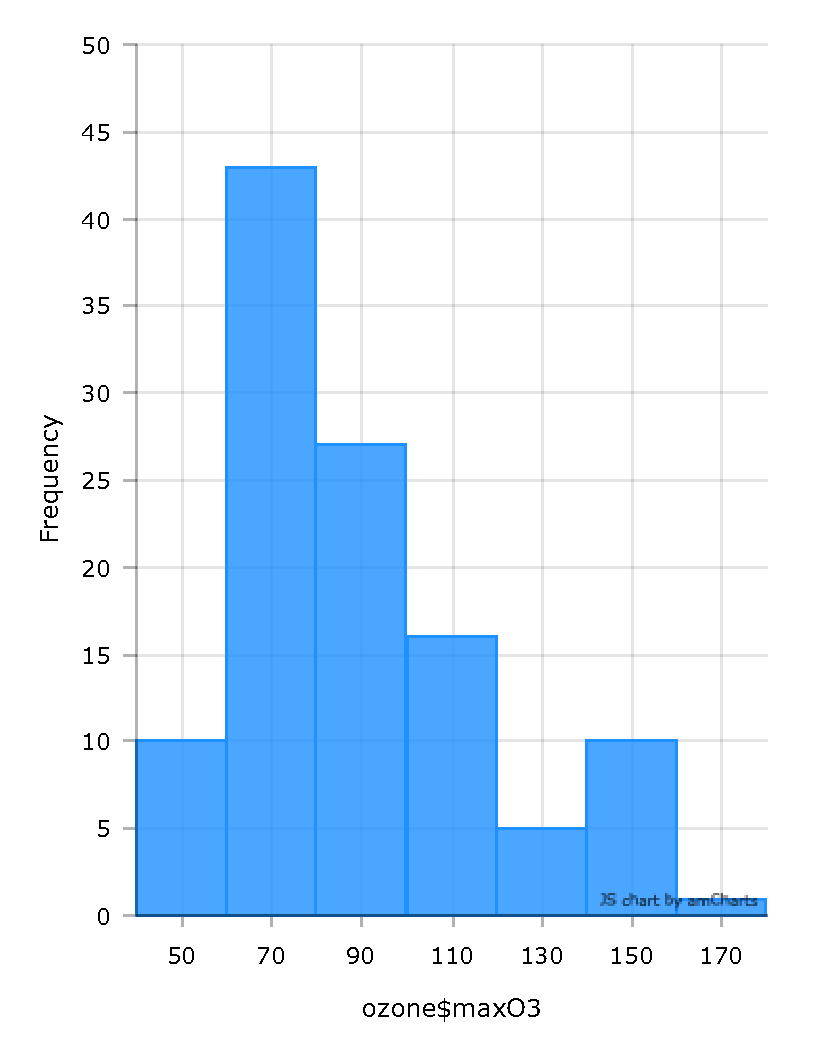
\includegraphics{TUTO_VISU_files/figure-latex/unnamed-chunk-11-1} \end{center}

\BeginKnitrBlock{exercise}[Tâches solaires]
\protect\hypertarget{exr:exo3}{}{\label{exr:exo3} \iffalse (Tâches solaires) \fi{} }
\EndKnitrBlock{exercise}

\begin{enumerate}
\def\labelenumi{\arabic{enumi}.}
\tightlist
\item
  Importer la série \textbf{taches\_solaires.csv} qui donne, date par date, un nombre de taches solaires observées.
\end{enumerate}

\begin{Shaded}
\begin{Highlighting}[]
\OperatorTok{>}\StringTok{ }\NormalTok{taches <-}\StringTok{ }\KeywordTok{read.table}\NormalTok{(}\StringTok{"taches_solaires.csv"}\NormalTok{,}\DataTypeTok{sep=}\StringTok{";"}\NormalTok{,}\DataTypeTok{header=}\OtherTok{TRUE}\NormalTok{,}\DataTypeTok{dec=}\StringTok{","}\NormalTok{)}
\end{Highlighting}
\end{Shaded}

\begin{enumerate}
\def\labelenumi{\arabic{enumi}.}
\setcounter{enumi}{1}
\tightlist
\item
  A l'aide de la fonction \textbf{cut\_interval} du tidyverse créer un facteur qui sépare l'intervalle d'années d'observation en 8 intervalles de tailles à peu près égales. On appellera \textbf{periode} ce facteur.
\end{enumerate}

\begin{Shaded}
\begin{Highlighting}[]
\OperatorTok{>}\StringTok{ }\KeywordTok{library}\NormalTok{(tidyverse)}
\OperatorTok{>}\StringTok{ }\NormalTok{periode <-}\StringTok{ }\KeywordTok{cut_interval}\NormalTok{(taches}\OperatorTok{$}\NormalTok{annee,}\DataTypeTok{n=}\DecValTok{8}\NormalTok{)}
\end{Highlighting}
\end{Shaded}

\begin{enumerate}
\def\labelenumi{\arabic{enumi}.}
\setcounter{enumi}{2}
\tightlist
\item
  Utiliser les levels suivants pour le facteur \textbf{periode}.
\end{enumerate}

\begin{Shaded}
\begin{Highlighting}[]
\OperatorTok{>}\StringTok{ }\NormalTok{couleurs <-}\StringTok{ }\KeywordTok{c}\NormalTok{(}\StringTok{"yellow"}\NormalTok{, }\StringTok{"magenta"}\NormalTok{, }\StringTok{"orange"}\NormalTok{, }\StringTok{"cyan"}\NormalTok{,}
\OperatorTok{+}\StringTok{               "grey"}\NormalTok{, }\StringTok{"red"}\NormalTok{, }\StringTok{"green"}\NormalTok{, }\StringTok{"blue"}\NormalTok{)}
\end{Highlighting}
\end{Shaded}

\begin{Shaded}
\begin{Highlighting}[]
\OperatorTok{>}\StringTok{ }\KeywordTok{levels}\NormalTok{(periode) <-}\StringTok{ }\NormalTok{couleurs}
\end{Highlighting}
\end{Shaded}

\begin{enumerate}
\def\labelenumi{\arabic{enumi}.}
\setcounter{enumi}{3}
\tightlist
\item
  Expliquer la sortie de la fonction
\end{enumerate}

\begin{Shaded}
\begin{Highlighting}[]
\OperatorTok{>}\StringTok{ }\NormalTok{coordx <-}\StringTok{ }\KeywordTok{seq}\NormalTok{(}\DataTypeTok{along=}\NormalTok{taches[,}\DecValTok{1}\NormalTok{])}
\end{Highlighting}
\end{Shaded}

\begin{enumerate}
\def\labelenumi{\arabic{enumi}.}
\setcounter{enumi}{4}
\tightlist
\item
  On crée une séquence avec un pas de 1 de longueur égale à la dimension de \texttt{taches{[},1{]}}. Visualiser la série du nombre de taches en utilisant une couleur différente pour chaque période.
\end{enumerate}

\begin{Shaded}
\begin{Highlighting}[]
\OperatorTok{>}\StringTok{ }\KeywordTok{plot}\NormalTok{(coordx,taches[,}\DecValTok{1}\NormalTok{],}\DataTypeTok{xlab=}\StringTok{"Temps"}\NormalTok{,}\DataTypeTok{ylab=}\StringTok{"Nombre de taches"}\NormalTok{,}
\OperatorTok{+}\StringTok{      }\DataTypeTok{col=}\NormalTok{periode,}\DataTypeTok{type=}\StringTok{"p"}\NormalTok{,}\DataTypeTok{pch=}\StringTok{"+"}\NormalTok{)}
\end{Highlighting}
\end{Shaded}

\begin{center}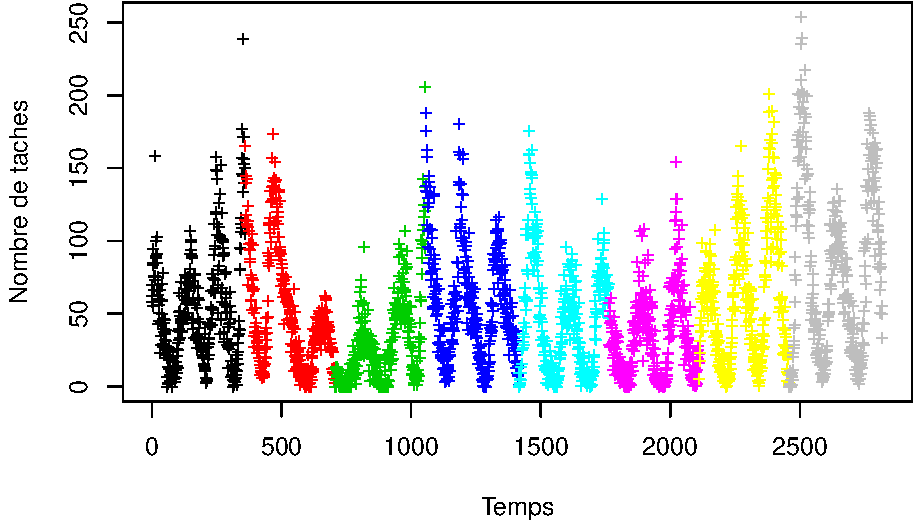
\includegraphics{TUTO_VISU_files/figure-latex/unnamed-chunk-17-1} \end{center}

\BeginKnitrBlock{exercise}[Layout]
\protect\hypertarget{exr:exo4}{}{\label{exr:exo4} \iffalse (Layout) \fi{} }On reprend le jeu de données sur l'ozone. A l'aide de la fonction \textbf{layout} séparer la fenêtre graphique en deux lignes avec
\EndKnitrBlock{exercise}

\begin{enumerate}
\def\labelenumi{\arabic{enumi}.}
\tightlist
\item
  un graphe sur la première ligne (nuage de points \textbf{maxO3 vs T12})
\item
  2 graphes sur la deuxième colonne (histogramme de \textbf{T12} et boxplot de \textbf{maxO3}).
\end{enumerate}

\begin{Shaded}
\begin{Highlighting}[]
\OperatorTok{>}\StringTok{ }\KeywordTok{layout}\NormalTok{(}\KeywordTok{matrix}\NormalTok{(}\KeywordTok{c}\NormalTok{(}\DecValTok{1}\NormalTok{,}\DecValTok{1}\NormalTok{,}\DecValTok{2}\NormalTok{,}\DecValTok{3}\NormalTok{), }\DecValTok{2}\NormalTok{, }\DecValTok{2}\NormalTok{, }\DataTypeTok{byrow =} \OtherTok{TRUE}\NormalTok{))}
\OperatorTok{>}\StringTok{ }\KeywordTok{plot}\NormalTok{(maxO3}\OperatorTok{~}\NormalTok{T12,}\DataTypeTok{data=}\NormalTok{ozone)}
\OperatorTok{>}\StringTok{ }\KeywordTok{hist}\NormalTok{(ozone}\OperatorTok{$}\NormalTok{T12)}
\OperatorTok{>}\StringTok{ }\KeywordTok{boxplot}\NormalTok{(ozone}\OperatorTok{$}\NormalTok{maxO3)}
\end{Highlighting}
\end{Shaded}

\begin{center}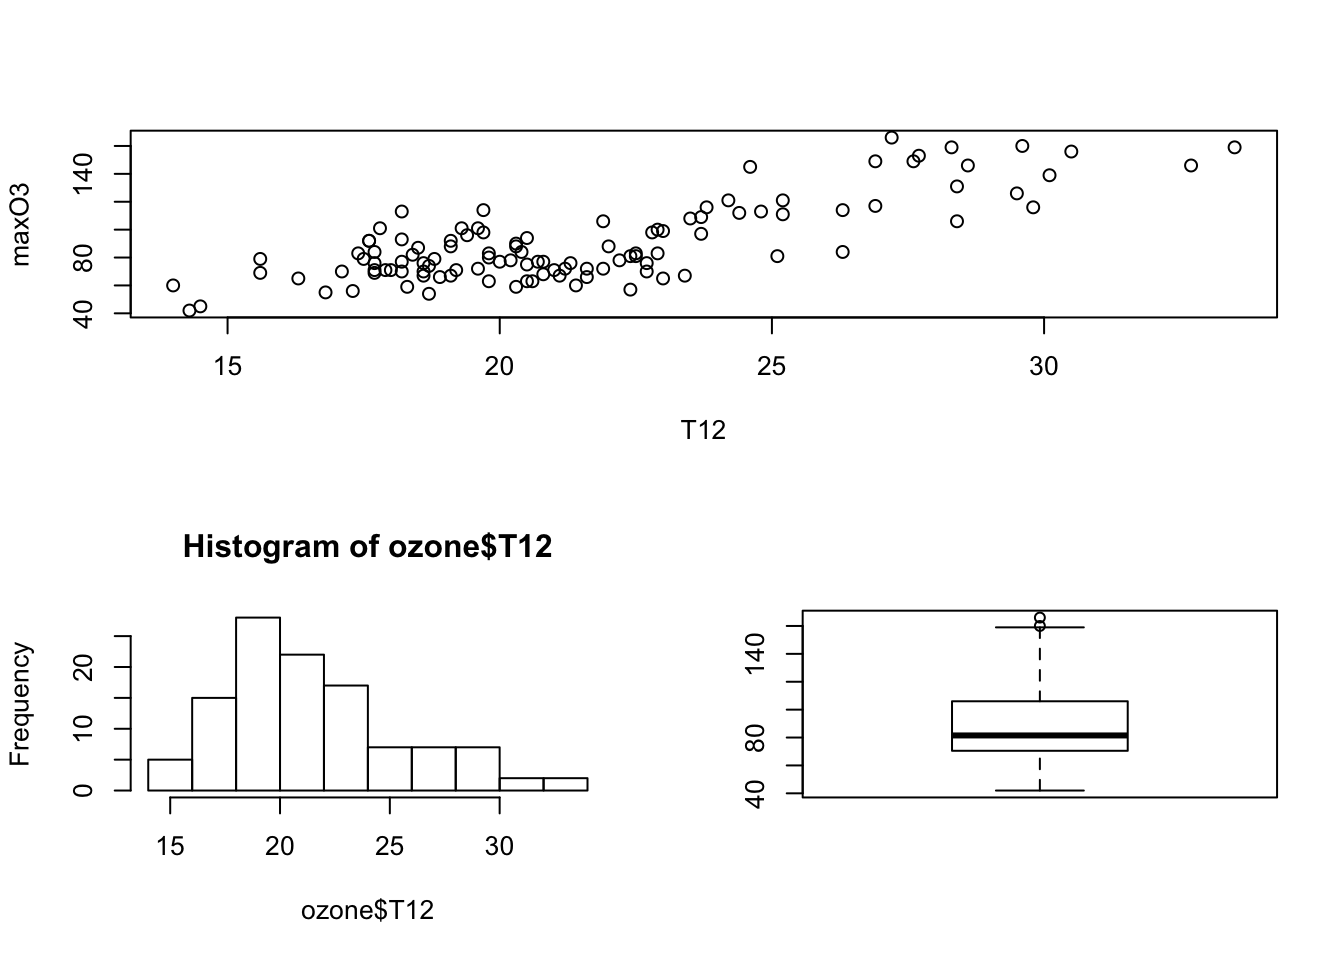
\includegraphics{TUTO_VISU_files/figure-latex/unnamed-chunk-18-1} \end{center}

\hypertarget{la-grammaire-ggplot2}{%
\section{\texorpdfstring{La grammaire \textbf{ggplot2}}{La grammaire ggplot2}}\label{la-grammaire-ggplot2}}

Ce package propose de définir des graphes sur \textbf{R} en utilisant une \textbf{grammaire des graphiques} (tout comme \textbf{dplyr} pour manipuler les données). On peut trouver de la documentation sur ce package aux url \url{http://ggplot2.org} et \url{https://ggplot2-book.org}.

\hypertarget{premiers-graphes-ggplot2}{%
\subsection{\texorpdfstring{Premiers graphes \texttt{ggplot2}}{Premiers graphes ggplot2}}\label{premiers-graphes-ggplot2}}

Nous considérons un sous échantillon du jeu de données \textbf{diamonds} du package \textbf{ggplot2} (qui se trouve dans le \textbf{tidyverse}).

\begin{Shaded}
\begin{Highlighting}[]
\OperatorTok{>}\StringTok{ }\KeywordTok{library}\NormalTok{(tidyverse)}
\OperatorTok{>}\StringTok{ }\KeywordTok{set.seed}\NormalTok{(}\DecValTok{1234}\NormalTok{)}
\OperatorTok{>}\StringTok{ }\NormalTok{diamonds2 <-}\StringTok{ }\NormalTok{diamonds[}\KeywordTok{sample}\NormalTok{(}\KeywordTok{nrow}\NormalTok{(diamonds),}\DecValTok{5000}\NormalTok{),] }
\OperatorTok{>}\StringTok{ }\KeywordTok{summary}\NormalTok{(diamonds2)}
\CommentTok{##      carat               cut       color       clarity         depth      }
\CommentTok{##  Min.   :0.2000   Fair     : 158   D: 640   SI1    :1189   Min.   :43.00  }
\CommentTok{##  1st Qu.:0.4000   Good     : 455   E: 916   VS2    :1157   1st Qu.:61.10  }
\CommentTok{##  Median :0.7000   Very Good:1094   F: 900   SI2    : 876   Median :61.80  }
\CommentTok{##  Mean   :0.7969   Premium  :1280   G:1018   VS1    : 738   Mean   :61.76  }
\CommentTok{##  3rd Qu.:1.0400   Ideal    :2013   H: 775   VVS2   : 470   3rd Qu.:62.50  }
\CommentTok{##  Max.   :4.1300                    I: 481   VVS1   : 326   Max.   :71.60  }
\CommentTok{##                                    J: 270   (Other): 244                  }
\CommentTok{##      table           price             x                y        }
\CommentTok{##  Min.   :49.00   Min.   :  365   Min.   : 0.000   Min.   :3.720  }
\CommentTok{##  1st Qu.:56.00   1st Qu.:  945   1st Qu.: 4.720   1st Qu.:4.720  }
\CommentTok{##  Median :57.00   Median : 2376   Median : 5.690   Median :5.700  }
\CommentTok{##  Mean   :57.43   Mean   : 3917   Mean   : 5.728   Mean   :5.731  }
\CommentTok{##  3rd Qu.:59.00   3rd Qu.: 5294   3rd Qu.: 6.530   3rd Qu.:6.520  }
\CommentTok{##  Max.   :95.00   Max.   :18757   Max.   :10.000   Max.   :9.850  }
\CommentTok{##                                                                  }
\CommentTok{##        z        }
\CommentTok{##  Min.   :0.000  }
\CommentTok{##  1st Qu.:2.920  }
\CommentTok{##  Median :3.520  }
\CommentTok{##  Mean   :3.538  }
\CommentTok{##  3rd Qu.:4.030  }
\CommentTok{##  Max.   :6.430  }
\CommentTok{## }
\OperatorTok{>}\StringTok{ }\KeywordTok{help}\NormalTok{(diamonds)}
\end{Highlighting}
\end{Shaded}

Pour un jeu de données considéré, un graphe \textbf{ggplot} est défini à partir de \textbf{couches} que l'on assemblera avec l'opérateur \texttt{+}. Il faut a minima spécifier :

\begin{itemize}
\tightlist
\item
  les données
\item
  les variables que l'on souhaite représenter
\item
  le type de représentation (nuage de points, boxplot\ldots{}).
\end{itemize}

Il existe un verbe pour définir chacune de ces couches :

\begin{itemize}
\tightlist
\item
  \textbf{ggplot} pour les données
\item
  \textbf{aes} (aesthetics) pour les variables
\item
  \textbf{geom\_} pour le type de représentation.
\end{itemize}

On peut obtenir le nuage de points \textbf{carat vs price} avec la fonction \textbf{plot} :

\begin{Shaded}
\begin{Highlighting}[]
\OperatorTok{>}\StringTok{ }\KeywordTok{plot}\NormalTok{(price}\OperatorTok{~}\NormalTok{carat,}\DataTypeTok{data=}\NormalTok{diamonds2)}
\end{Highlighting}
\end{Shaded}

\begin{center}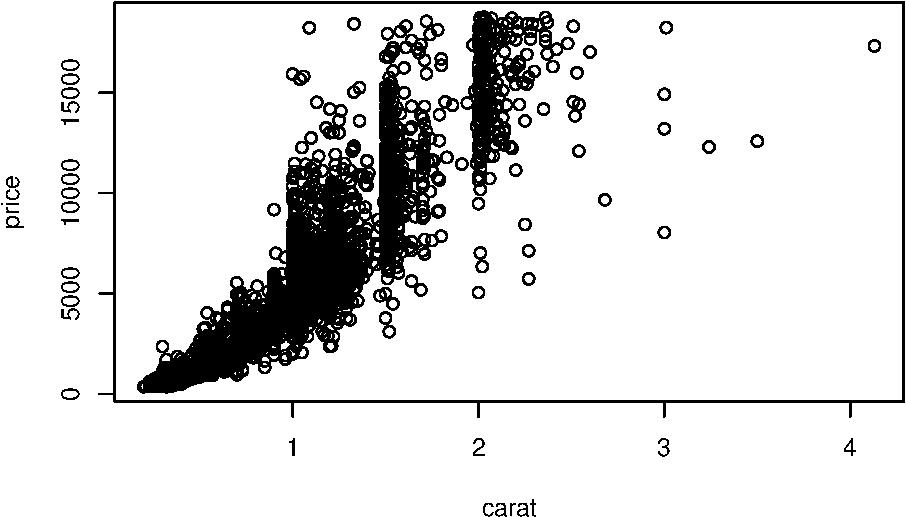
\includegraphics{TUTO_VISU_files/figure-latex/unnamed-chunk-20-1} \end{center}

Avec \textbf{ggplot}, on va faire

\begin{Shaded}
\begin{Highlighting}[]
\OperatorTok{>}\StringTok{ }\KeywordTok{ggplot}\NormalTok{(diamonds2) }\CommentTok{#rien}
\end{Highlighting}
\end{Shaded}

\begin{center}
\includegraphics{TUTO_VISU_files/figure-latex/unnamed-chunk-21-1} \end{center}

\begin{Shaded}
\begin{Highlighting}[]
\OperatorTok{>}\StringTok{ }\KeywordTok{ggplot}\NormalTok{(diamonds2)}\OperatorTok{+}\KeywordTok{aes}\NormalTok{(}\DataTypeTok{x=}\NormalTok{carat,}\DataTypeTok{y=}\NormalTok{price) }\CommentTok{#rien}
\end{Highlighting}
\end{Shaded}

\begin{center}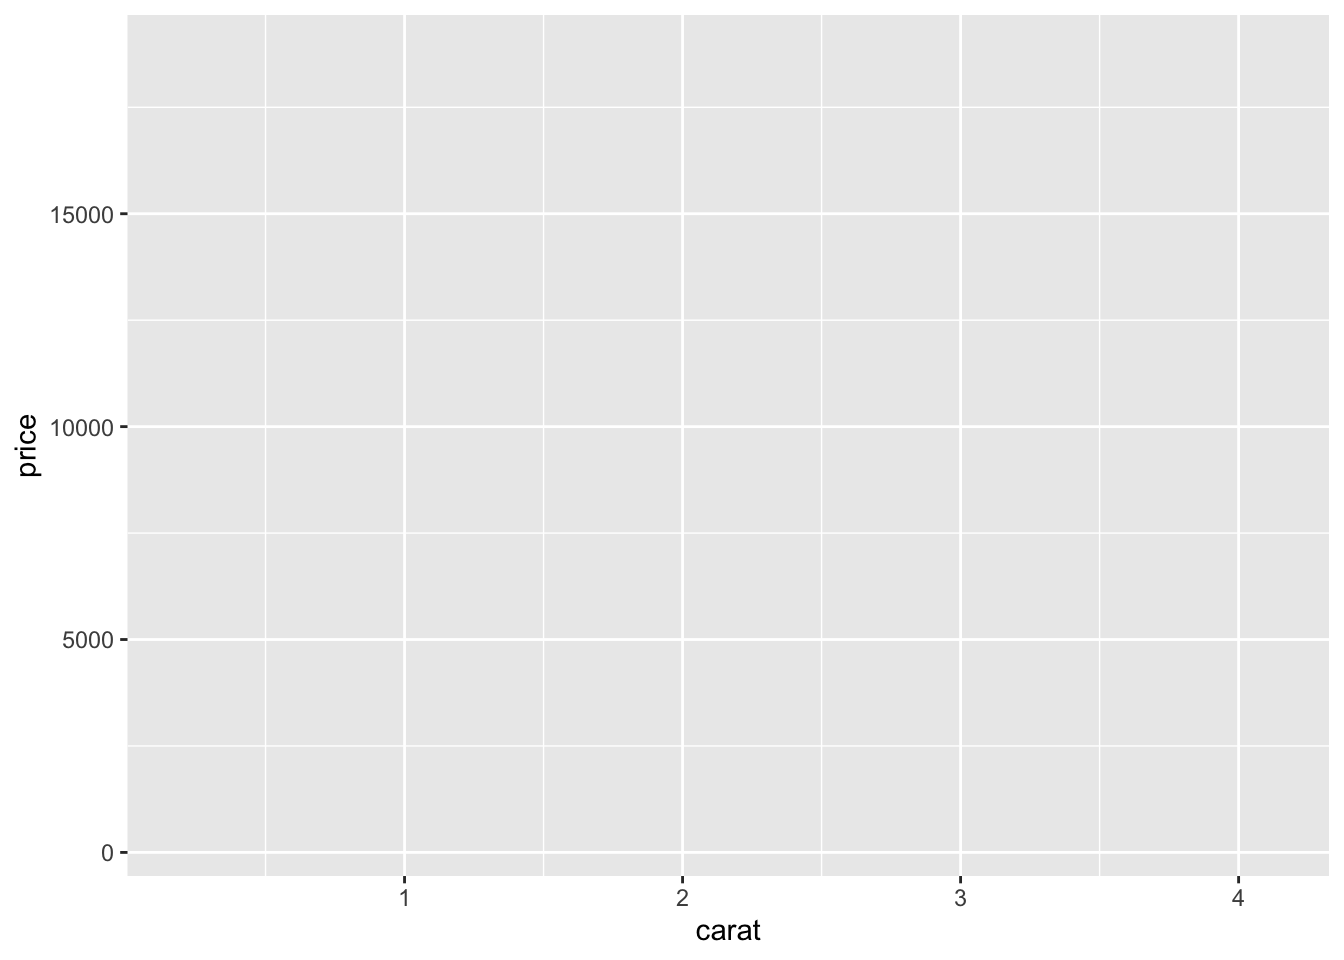
\includegraphics{TUTO_VISU_files/figure-latex/unnamed-chunk-21-2} \end{center}

\begin{Shaded}
\begin{Highlighting}[]
\OperatorTok{>}\StringTok{ }\KeywordTok{ggplot}\NormalTok{(diamonds2)}\OperatorTok{+}\KeywordTok{aes}\NormalTok{(}\DataTypeTok{x=}\NormalTok{carat,}\DataTypeTok{y=}\NormalTok{price)}\OperatorTok{+}\KeywordTok{geom_point}\NormalTok{() }\CommentTok{#bon}
\end{Highlighting}
\end{Shaded}

\begin{center}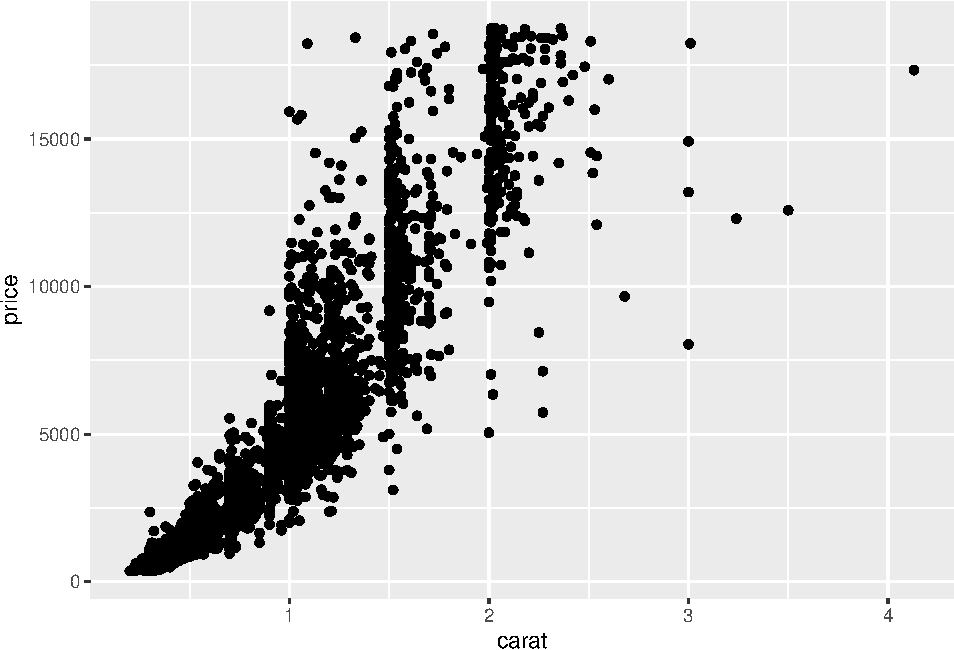
\includegraphics{TUTO_VISU_files/figure-latex/unnamed-chunk-21-3} \end{center}

\BeginKnitrBlock{exercise}[Permiers graphes ggplot]
\protect\hypertarget{exr:exoggplot1}{}{\label{exr:exoggplot1} \iffalse (Permiers graphes ggplot) \fi{} }
\EndKnitrBlock{exercise}

\begin{enumerate}
\def\labelenumi{\arabic{enumi}.}
\tightlist
\item
  Tracer l'histogramme de la variable \textbf{carat} (utiliser \texttt{geom\_histogram}).
\item
  Tracer l'histogramme de la variable \textbf{carat} avec 10 classes (\textbf{help(geom\_histogram)}).
\item
  Tracer le diagramme à batons de la variable \textbf{cut} (utiliser \textbf{geom\_bar}).
\end{enumerate}

\begin{Shaded}
\begin{Highlighting}[]
\OperatorTok{>}\StringTok{ }\KeywordTok{ggplot}\NormalTok{(diamonds2)}\OperatorTok{+}\KeywordTok{aes}\NormalTok{(}\DataTypeTok{x=}\NormalTok{carat)}\OperatorTok{+}\KeywordTok{geom_histogram}\NormalTok{()}
\end{Highlighting}
\end{Shaded}

\begin{center}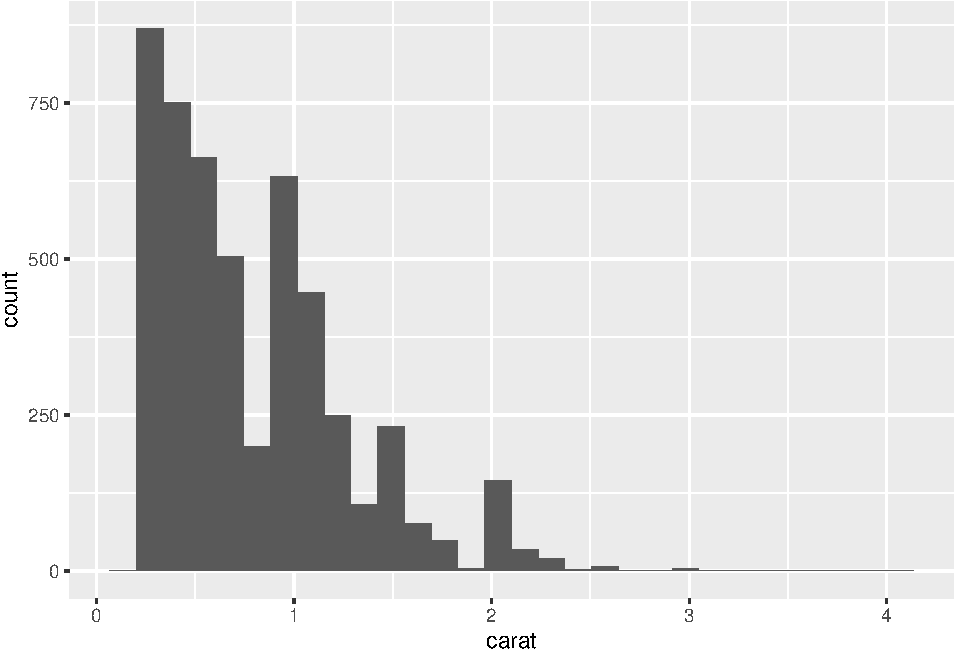
\includegraphics{TUTO_VISU_files/figure-latex/unnamed-chunk-22-1} \end{center}

\begin{Shaded}
\begin{Highlighting}[]
\OperatorTok{>}\StringTok{ }\KeywordTok{ggplot}\NormalTok{(diamonds2)}\OperatorTok{+}\KeywordTok{aes}\NormalTok{(}\DataTypeTok{x=}\NormalTok{carat)}\OperatorTok{+}\KeywordTok{geom_histogram}\NormalTok{(}\DataTypeTok{bins=}\DecValTok{10}\NormalTok{)}
\end{Highlighting}
\end{Shaded}

\begin{center}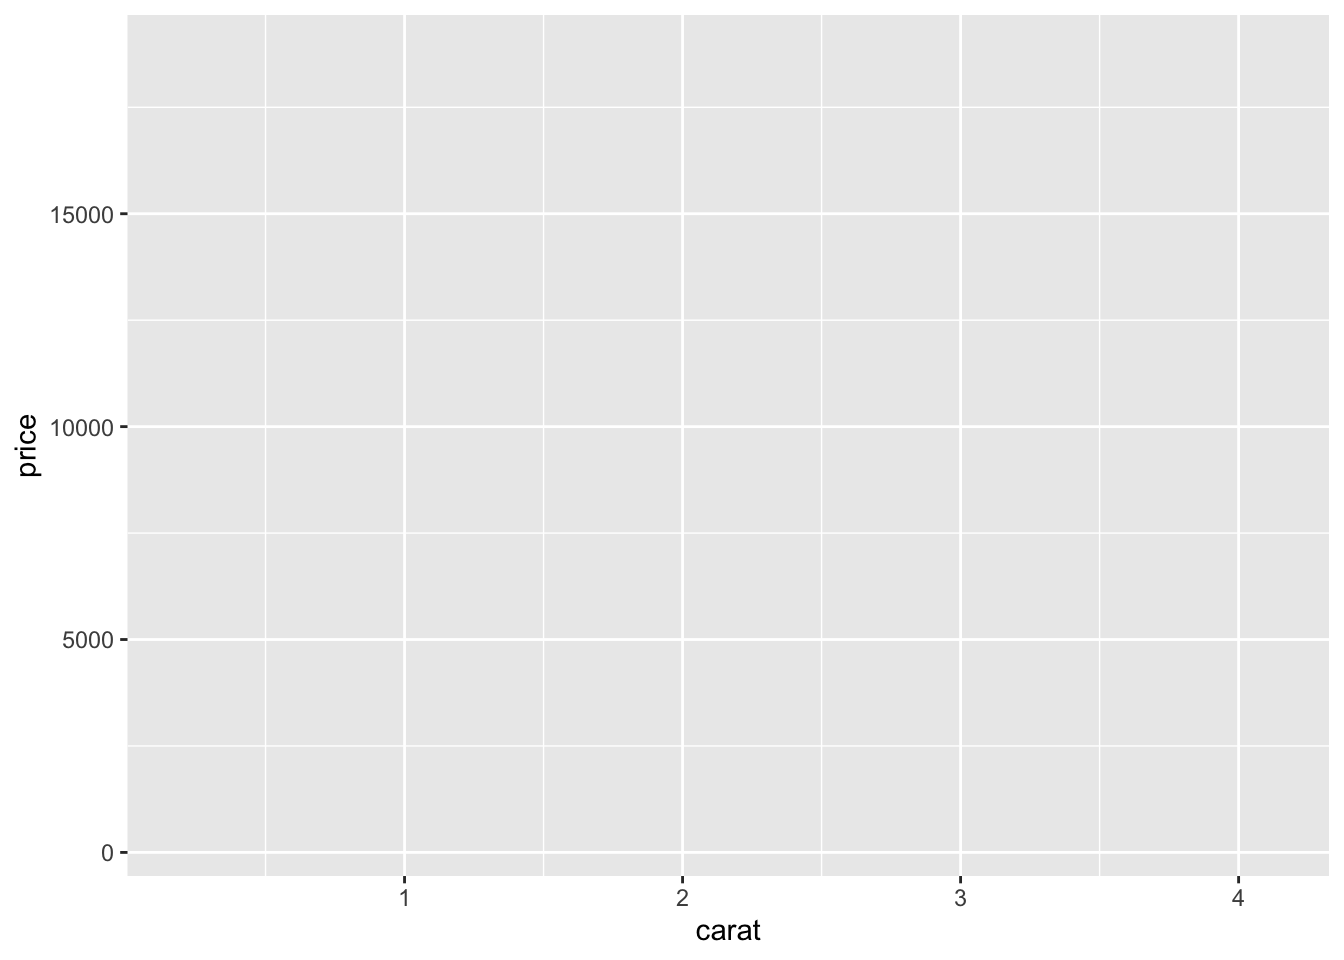
\includegraphics{TUTO_VISU_files/figure-latex/unnamed-chunk-22-2} \end{center}

\begin{Shaded}
\begin{Highlighting}[]
\OperatorTok{>}\StringTok{ }\KeywordTok{ggplot}\NormalTok{(diamonds2)}\OperatorTok{+}\KeywordTok{aes}\NormalTok{(}\DataTypeTok{x=}\NormalTok{cut)}\OperatorTok{+}\KeywordTok{geom_bar}\NormalTok{()}
\end{Highlighting}
\end{Shaded}

\begin{center}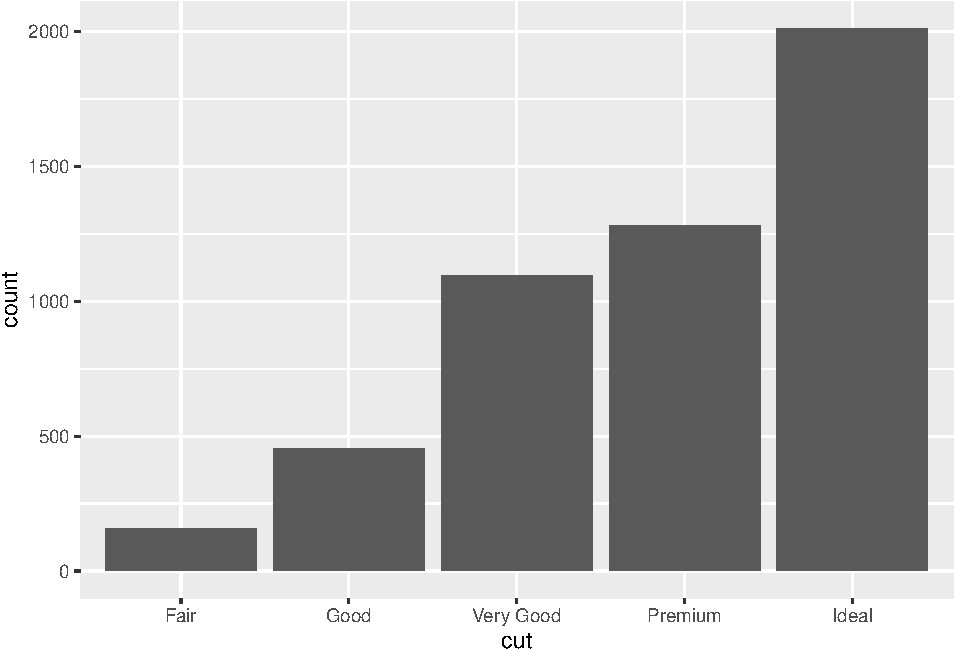
\includegraphics{TUTO_VISU_files/figure-latex/unnamed-chunk-22-3} \end{center}

La syntaxe \textbf{ggplot} se construit à partir d'éléments indépendants qui définissent la grammaire de \textbf{ggplot}. Les principaux verbes sont :

\begin{itemize}
\tightlist
\item
  \textbf{Data} (\texttt{ggplot}) : les données au format \textbf{dataframe} ou \textbf{tibble}
\item
  \textbf{Aesthetics} (\texttt{aes}) : pour sépecifier les variables à représenter dans le graphe.
\item
  \textbf{Geometrics} (\texttt{geom\_...}) : le type de graphe (nuage de points, histogramme\ldots{}).
\item
  \textbf{Statistics} (\texttt{stat\_...}) : utile pour spécifier des transformations des données nécessaires pour obtenir le graphe.
\item
  \textbf{Scales} (\texttt{scale\_...}) : pour controler les paramètres permettant d'affiner le graphe (changement de couleurs, paramètres des axes\ldots{}).
\end{itemize}

Tous ces éléments sont reliés avec le symbole \textbf{+}.

\hypertarget{data-et-aesthetics}{%
\subsection{Data et aesthetics}\label{data-et-aesthetics}}

Ces deux verbes sont à utiliser pour tous les graphes \textbf{ggplot}. Le verbe \textbf{ggplot} servira à définir le jeu de données que l'on souhaite utiliser. Si le code est bien fait, nous n'aurons plus à utiliser le nom du jeu de données par la suite pour construire le graphe. Le verbe \texttt{aes} est quant à lui utile pour sépcifier le nom des variables que l'on souhaite visualiser. Par exemple, pour le nuage de points \textbf{price vs carat} la syntaxe devra débuter par

\begin{Shaded}
\begin{Highlighting}[]
\OperatorTok{>}\StringTok{ }\KeywordTok{ggplot}\NormalTok{(diamonds2)}\OperatorTok{+}\KeywordTok{aes}\NormalTok{(}\DataTypeTok{x=}\NormalTok{carat,}\DataTypeTok{y=}\NormalTok{price)}
\end{Highlighting}
\end{Shaded}

Les variables peuvent également être utilisées pour colorier des points ou des barres, définir des tailles\ldots{} Dans ce cas on pourra renseigner les arguments \textbf{color}, \textbf{size}, \textbf{fill} dans la fonction \textbf{aes}. Par exemple

\begin{Shaded}
\begin{Highlighting}[]
\OperatorTok{>}\StringTok{ }\KeywordTok{ggplot}\NormalTok{(diamonds2)}\OperatorTok{+}\KeywordTok{aes}\NormalTok{(}\DataTypeTok{x=}\NormalTok{carat,}\DataTypeTok{y=}\NormalTok{price,}\DataTypeTok{color=}\NormalTok{cut)}
\end{Highlighting}
\end{Shaded}

\hypertarget{geometrics}{%
\subsection{\texorpdfstring{\texttt{Geometrics}}{Geometrics}}\label{geometrics}}

Ce verbe décrira le type de représentation souhaitée. Pour un nuage de points, on utilisera par exemple \textbf{geom\_point} :

\begin{Shaded}
\begin{Highlighting}[]
\OperatorTok{>}\StringTok{ }\KeywordTok{ggplot}\NormalTok{(diamonds2)}\OperatorTok{+}\KeywordTok{aes}\NormalTok{(}\DataTypeTok{x=}\NormalTok{carat,}\DataTypeTok{y=}\NormalTok{price,}\DataTypeTok{color=}\NormalTok{cut)}\OperatorTok{+}\KeywordTok{geom_point}\NormalTok{()}
\end{Highlighting}
\end{Shaded}

\begin{center}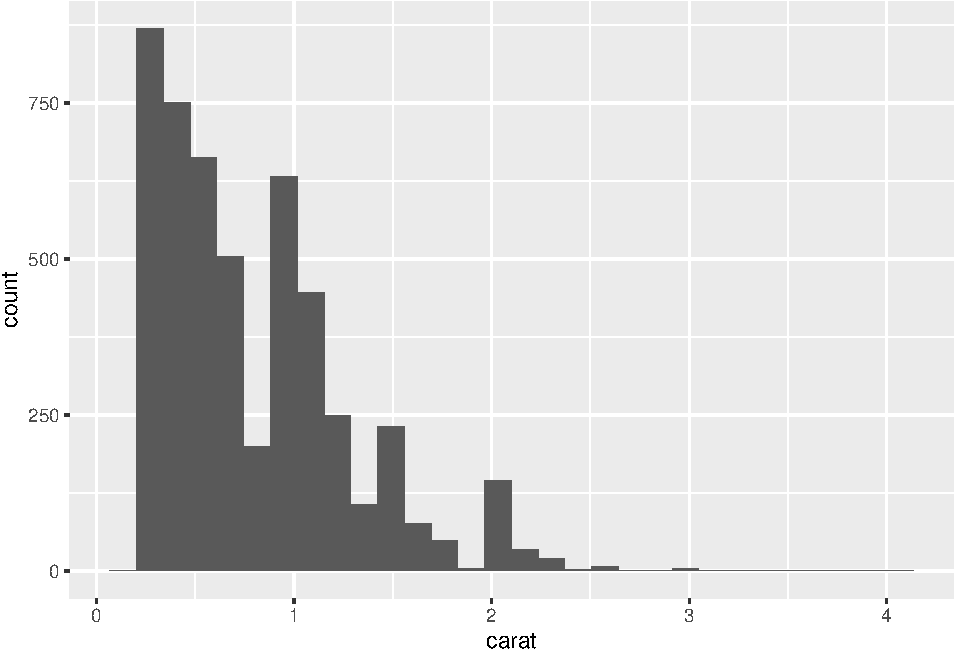
\includegraphics{TUTO_VISU_files/figure-latex/unnamed-chunk-25-1} \end{center}

On observe que \textbf{ggplot} ajoute la légende automatiquement. Voici les principaux exemples de \textbf{geometrics} :

\begin{longtable}[]{@{}lll@{}}
\caption{\label{tab:geom} Principaux geometrics}\tabularnewline
\toprule
Geom & Description & Aesthetics\tabularnewline
\midrule
\endfirsthead
\toprule
Geom & Description & Aesthetics\tabularnewline
\midrule
\endhead
geom\_point() & nuage de points & x, y, shape, fill\tabularnewline
geom\_line() & Ligne (ordonnée selon x) & x, y, linetype\tabularnewline
geom\_abline() & Ligne & slope, intercept\tabularnewline
geom\_path() & Ligne (ordonnée par l'index) & x, y, linetype\tabularnewline
geom\_text() & Texte & x, y, label, hjust, vjust\tabularnewline
geom\_rect() & Rectangle & xmin, xmax, ymin, ymax, fill, linetype\tabularnewline
geom\_polygon() & Polygone & x, y, fill, linetype\tabularnewline
geom\_segment() & Segment & x, y, xend, yend, fill, linetype\tabularnewline
geom\_bar() & Diaggramme en barres & x, fill, linetype, weight\tabularnewline
geom\_histogram() & Histogramme & x, fill, linetype, weight\tabularnewline
geom\_boxplot() & Boxplot & x, fill, weight\tabularnewline
geom\_density() & Densité & x, y, fill, linetype\tabularnewline
geom\_contour() & Lignes de contour & x, y, fill, linetype\tabularnewline
geom\_smooth() & Lisseur (linéaire ou non linéaire) & x, y, fill, linetype\tabularnewline
Tous & & color, size, group\tabularnewline
\bottomrule
\end{longtable}

\BeginKnitrBlock{exercise}[Diagrammes en barres]
\protect\hypertarget{exr:exoggplot2}{}{\label{exr:exoggplot2} \iffalse (Diagrammes en barres) \fi{} }
\EndKnitrBlock{exercise}

\begin{enumerate}
\def\labelenumi{\arabic{enumi}.}
\tightlist
\item
  Tracer le diagramme en barres de la variable \textbf{cut} avec des barres bleues.
\item
  Tracer le diagramme en barres de la variable \textbf{cut} avec une couleur pour chaque modalité de \textbf{cut} ainsi qu'une légende qui permet de repérer la couleur.
\item
  Tracer le diagramme en barres de la variable \textbf{cut} avec une couleur pour chaque modalité que vous choisirez (et sans légende).
\end{enumerate}

\begin{Shaded}
\begin{Highlighting}[]
\OperatorTok{>}\StringTok{ }\KeywordTok{ggplot}\NormalTok{(diamonds2)}\OperatorTok{+}\KeywordTok{aes}\NormalTok{(}\DataTypeTok{x=}\NormalTok{cut)}\OperatorTok{+}\KeywordTok{geom_bar}\NormalTok{(}\DataTypeTok{fill=}\StringTok{"blue"}\NormalTok{)}
\end{Highlighting}
\end{Shaded}

\begin{center}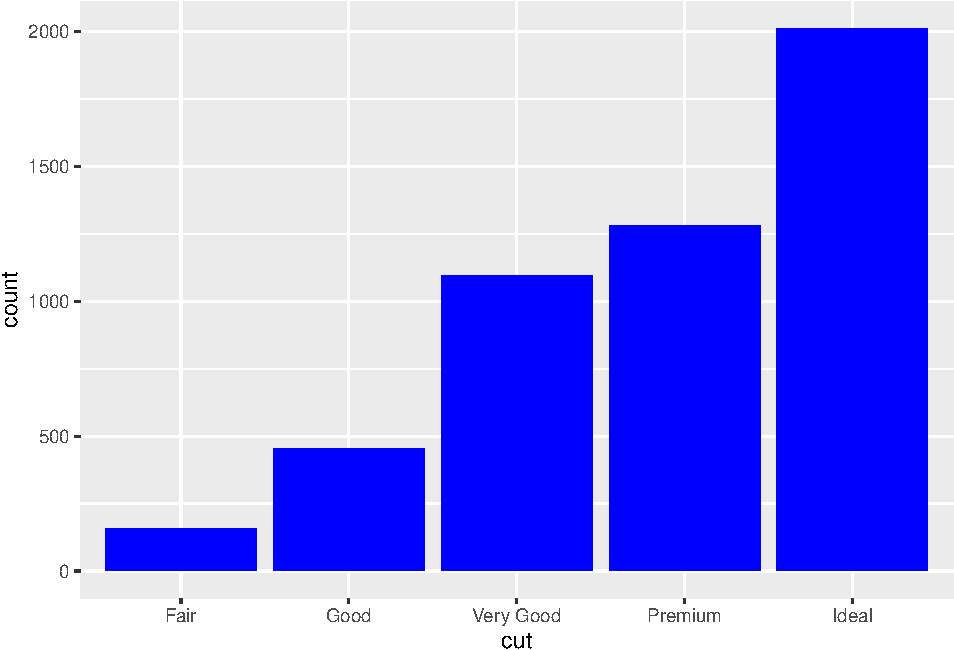
\includegraphics{TUTO_VISU_files/figure-latex/unnamed-chunk-26-1} \end{center}

\begin{Shaded}
\begin{Highlighting}[]
\OperatorTok{>}\StringTok{ }\KeywordTok{ggplot}\NormalTok{(diamonds2)}\OperatorTok{+}\KeywordTok{aes}\NormalTok{(}\DataTypeTok{x=}\NormalTok{cut,}\DataTypeTok{fill=}\NormalTok{cut)}\OperatorTok{+}\KeywordTok{geom_bar}\NormalTok{()}
\end{Highlighting}
\end{Shaded}

\begin{center}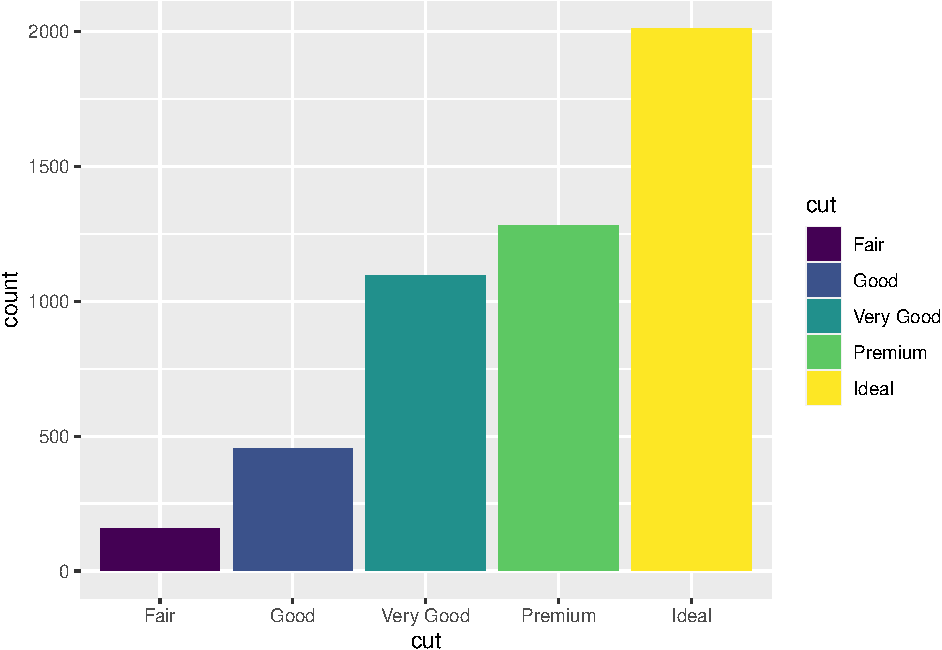
\includegraphics{TUTO_VISU_files/figure-latex/unnamed-chunk-26-2} \end{center}

\begin{Shaded}
\begin{Highlighting}[]
\OperatorTok{>}\StringTok{ }\KeywordTok{ggplot}\NormalTok{(diamonds2)}\OperatorTok{+}\KeywordTok{aes}\NormalTok{(}\DataTypeTok{x=}\NormalTok{cut)}\OperatorTok{+}\KeywordTok{geom_bar}\NormalTok{(}\DataTypeTok{fill=}\KeywordTok{c}\NormalTok{(}\StringTok{"blue"}\NormalTok{,}\StringTok{"red"}\NormalTok{,}\StringTok{"green"}\NormalTok{,}\StringTok{"yellow"}\NormalTok{,}\StringTok{"black"}\NormalTok{))}
\end{Highlighting}
\end{Shaded}

\begin{center}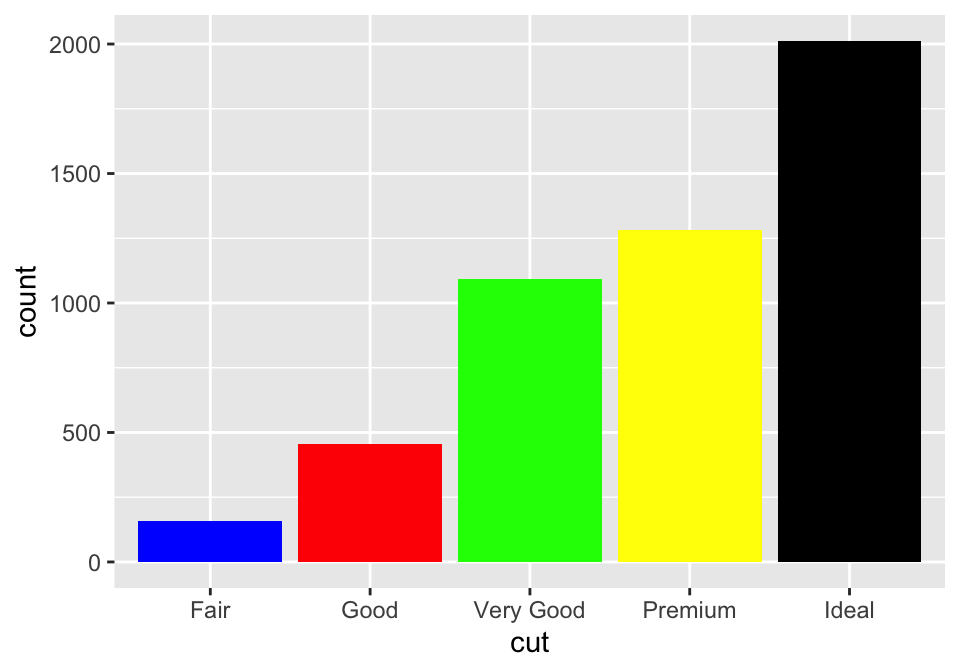
\includegraphics{TUTO_VISU_files/figure-latex/unnamed-chunk-26-3} \end{center}

\hypertarget{statistics}{%
\subsection{\texorpdfstring{\texttt{Statistics}}{Statistics}}\label{statistics}}

Certains graphes nécessitent des calculs d'indicateurs statistiques pour être tracé. C'est par exemple le cas pour le diagamme en barres et l'histogramme où il faut calculer des hauteurs des barres. Les transformations simples peuvent se faire rapidement, on peut par exemple tracer la fonction \textbf{sinus} avec

\begin{Shaded}
\begin{Highlighting}[]
\OperatorTok{>}\StringTok{ }\NormalTok{D <-}\StringTok{ }\KeywordTok{data.frame}\NormalTok{(}\DataTypeTok{X=}\KeywordTok{seq}\NormalTok{(}\OperatorTok{-}\DecValTok{2}\OperatorTok{*}\NormalTok{pi,}\DecValTok{2}\OperatorTok{*}\NormalTok{pi,}\DataTypeTok{by=}\FloatTok{0.01}\NormalTok{))}
\OperatorTok{>}\StringTok{ }\KeywordTok{ggplot}\NormalTok{(D)}\OperatorTok{+}\KeywordTok{aes}\NormalTok{(}\DataTypeTok{x=}\NormalTok{X,}\DataTypeTok{y=}\KeywordTok{sin}\NormalTok{(X))}\OperatorTok{+}\KeywordTok{geom_line}\NormalTok{()}
\end{Highlighting}
\end{Shaded}

\begin{center}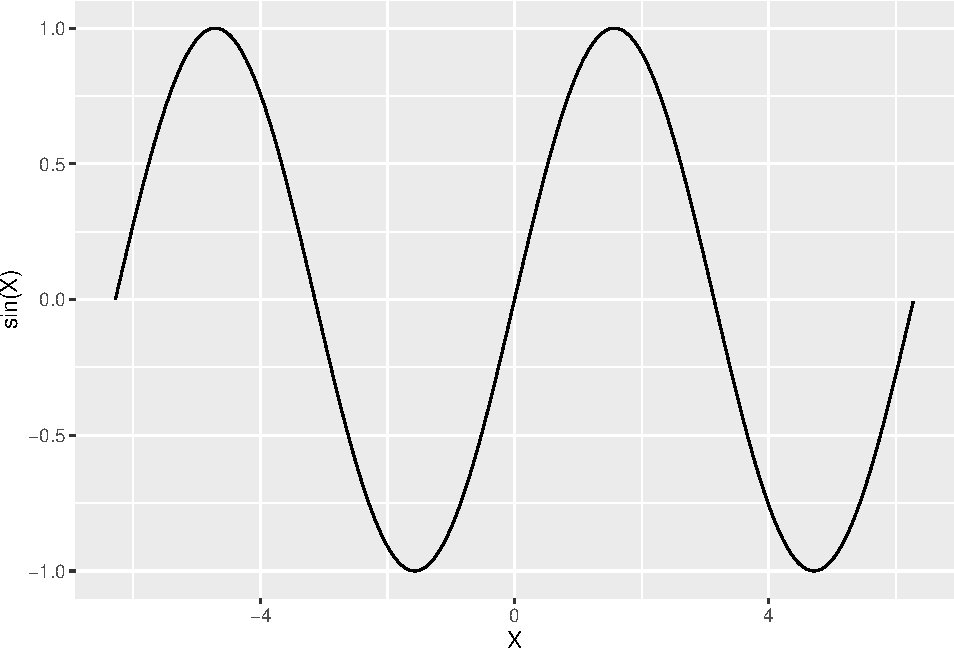
\includegraphics{TUTO_VISU_files/figure-latex/unnamed-chunk-27-1} \end{center}

La transformation est spécifiée dans la fonction \texttt{aes}. Pour des transformations plus complexes, nous devons utiliser des \textbf{statistics}. Une fonction \textbf{stat} permet de définir des nouvelles variables à partir du jeu de données initial, il est ensuite possible de représenter ces nouvelles variables.
Par exemple, la fonction \textbf{stat\_bin}, qui est utilisée par défaut pour construire des histogrammes, produit les variables suivantes :

\begin{itemize}
\tightlist
\item
  \texttt{count}, le nombre d'observations dans chaque classes.
\item
  \texttt{density}, la valeur de la densité des observations dans chaque classe (fréquance divisée par largeur de la classe).
\item
  \texttt{x}, le centre de la classe.
\end{itemize}

Par défaut \emph{geom\_histogram} fait appel à cette fonction \texttt{stat\_bin}et représente sur l'axe \(y\) le nombre d'observations dans chaque classe (la variable \textbf{count}).

\begin{Shaded}
\begin{Highlighting}[]
\OperatorTok{>}\StringTok{ }\KeywordTok{ggplot}\NormalTok{(diamonds2)}\OperatorTok{+}\KeywordTok{aes}\NormalTok{(}\DataTypeTok{x=}\NormalTok{price)}\OperatorTok{+}\KeywordTok{geom_histogram}\NormalTok{(}\DataTypeTok{bins=}\DecValTok{40}\NormalTok{)}
\end{Highlighting}
\end{Shaded}

\begin{center}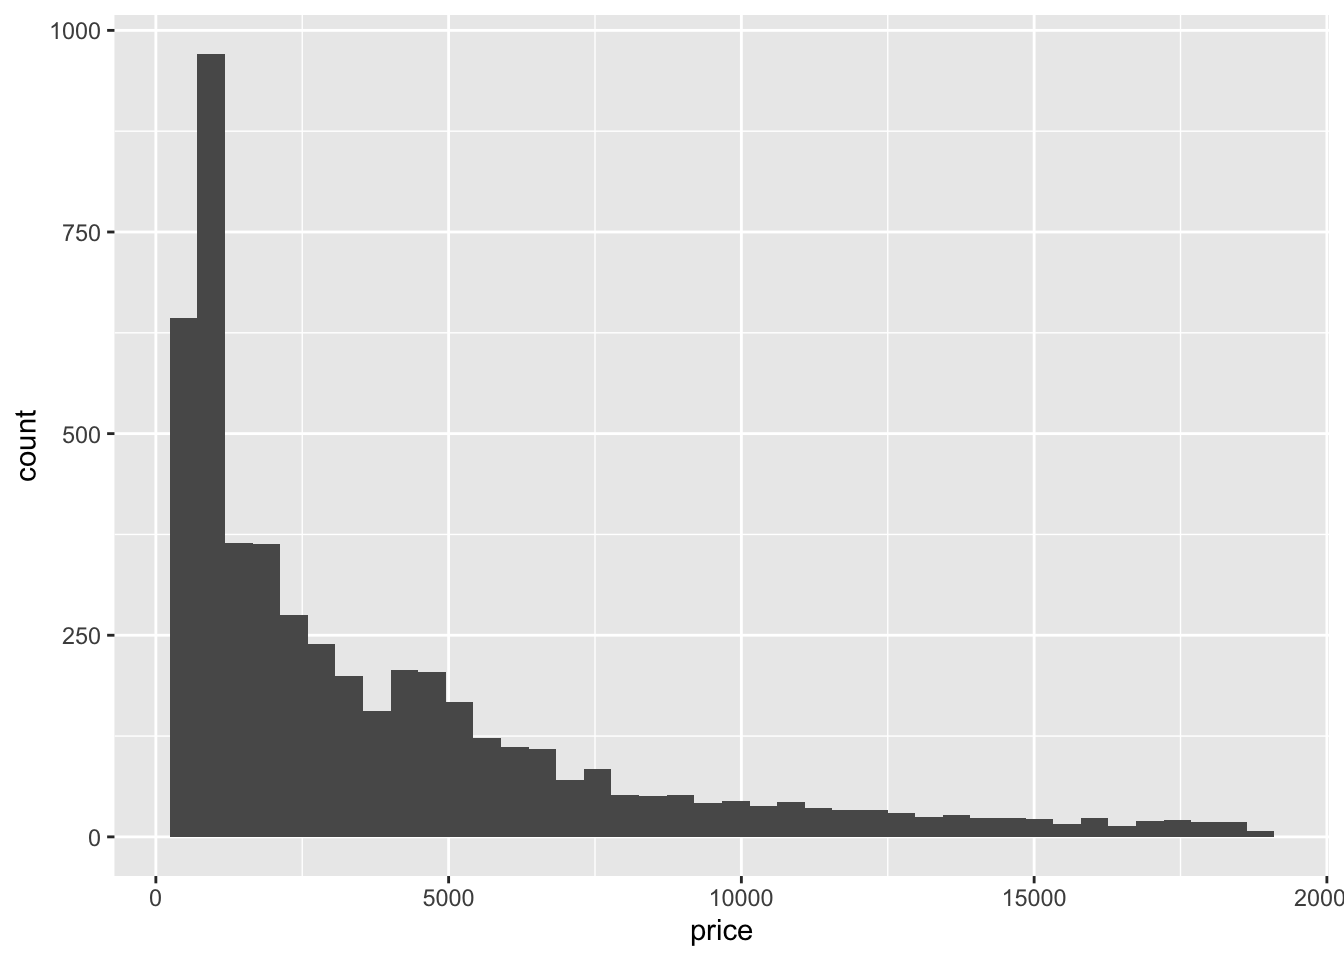
\includegraphics{TUTO_VISU_files/figure-latex/unnamed-chunk-28-1} \end{center}

Si on souhaite une autre variable issue de \texttt{stat\_bin}, comme par exemple la densité, il faudra utiliser

\begin{Shaded}
\begin{Highlighting}[]
\OperatorTok{>}\StringTok{ }\KeywordTok{ggplot}\NormalTok{(diamonds2)}\OperatorTok{+}\KeywordTok{aes}\NormalTok{(}\DataTypeTok{x=}\NormalTok{price,}\DataTypeTok{y=}\NormalTok{..density..)}\OperatorTok{+}\KeywordTok{geom_histogram}\NormalTok{(}\DataTypeTok{bins=}\DecValTok{40}\NormalTok{)}
\end{Highlighting}
\end{Shaded}

\begin{center}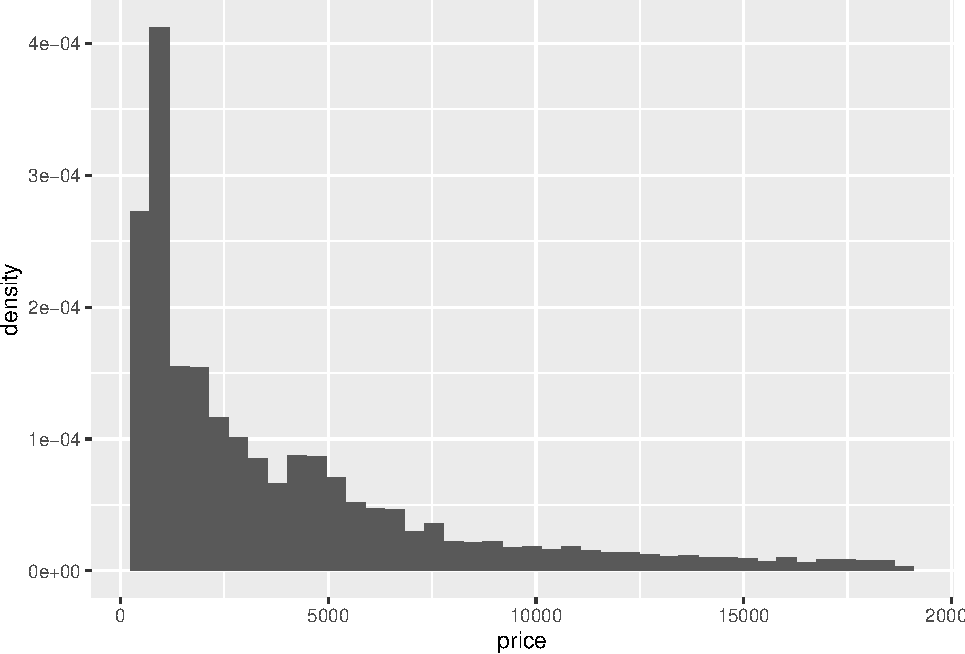
\includegraphics{TUTO_VISU_files/figure-latex/unnamed-chunk-29-1} \end{center}

Il est possible d'utiliser les fonctions \textbf{stat\_} à la place des \textbf{geom\_} pour certaines représentations. Chaque fonction \textbf{stat\_} possède par défaut un \textbf{geom\_} et réciproquement. On peut par exemple obtenir le même graphe que précédemment avec

\begin{Shaded}
\begin{Highlighting}[]
\OperatorTok{>}\StringTok{ }\KeywordTok{ggplot}\NormalTok{(diamonds2)}\OperatorTok{+}\KeywordTok{aes}\NormalTok{(}\DataTypeTok{x=}\NormalTok{price,}\DataTypeTok{y=}\NormalTok{..density..)}\OperatorTok{+}\KeywordTok{stat_bin}\NormalTok{()}
\end{Highlighting}
\end{Shaded}

Voici quelques exemple de fonctions \textbf{stat\_}

\begin{longtable}[]{@{}lll@{}}
\caption{\label{tab:ggplot-stat} Exemples de statistics.}\tabularnewline
\toprule
Stat & Description & Paramètres\tabularnewline
\midrule
\endfirsthead
\toprule
Stat & Description & Paramètres\tabularnewline
\midrule
\endhead
stat\_identity() & aucune transformation &\tabularnewline
stat\_bin() & Count & binwidth, origin\tabularnewline
stat\_density() & Density & adjust, kernel\tabularnewline
stat\_smooth() & Smoother & method, se\tabularnewline
stat\_boxplot() & Boxplot & coef\tabularnewline
\bottomrule
\end{longtable}

\emph{stat} et \emph{geom} ne sont pas toujours simples à combiner. Nous recommandons d'utiliser \textbf{geom} lorsqu'on débute avec \textbf{ggplot}, les \texttt{statistics}par défaut ne doivent en effet être changés que rarement.

\BeginKnitrBlock{exercise}[Diagramme en barres "très simple"...]
\protect\hypertarget{exr:exo-stat1}{}{\label{exr:exo-stat1} \iffalse (Diagramme en barres ``très simple''\ldots{}) \fi{} }
\EndKnitrBlock{exercise}

On considère une variable qualitative \(X\) dont la loi est donnée par
\[P(X=red)=0.3,\ P(X=blue)=0.2,\ P(X=green)=0.4,\ P(X=black)=0.1\]
Représenter cette distribution de probabilité avec un diagramme en barres.

\begin{Shaded}
\begin{Highlighting}[]
\OperatorTok{>}\StringTok{ }\NormalTok{X <-}\StringTok{ }\KeywordTok{data.frame}\NormalTok{(}\DataTypeTok{X1=}\KeywordTok{c}\NormalTok{(}\StringTok{"red"}\NormalTok{,}\StringTok{"blue"}\NormalTok{,}\StringTok{"green"}\NormalTok{,}\StringTok{"black"}\NormalTok{),}\DataTypeTok{prob=}\KeywordTok{c}\NormalTok{(}\FloatTok{0.3}\NormalTok{,}\FloatTok{0.2}\NormalTok{,}\FloatTok{0.4}\NormalTok{,}\FloatTok{0.1}\NormalTok{))}
\OperatorTok{>}\StringTok{ }\KeywordTok{ggplot}\NormalTok{(X)}\OperatorTok{+}\KeywordTok{aes}\NormalTok{(}\DataTypeTok{x=}\NormalTok{X1,}\DataTypeTok{y=}\NormalTok{prob,}\DataTypeTok{fill=}\NormalTok{X1)}\OperatorTok{+}\KeywordTok{geom_bar}\NormalTok{(}\DataTypeTok{stat=}\StringTok{"identity"}\NormalTok{)}\OperatorTok{+}
\OperatorTok{+}\StringTok{   }\KeywordTok{labs}\NormalTok{(}\DataTypeTok{fill=}\StringTok{"Couleur"}\NormalTok{)}\OperatorTok{+}\KeywordTok{xlab}\NormalTok{(}\StringTok{""}\NormalTok{)}
\end{Highlighting}
\end{Shaded}

\begin{center}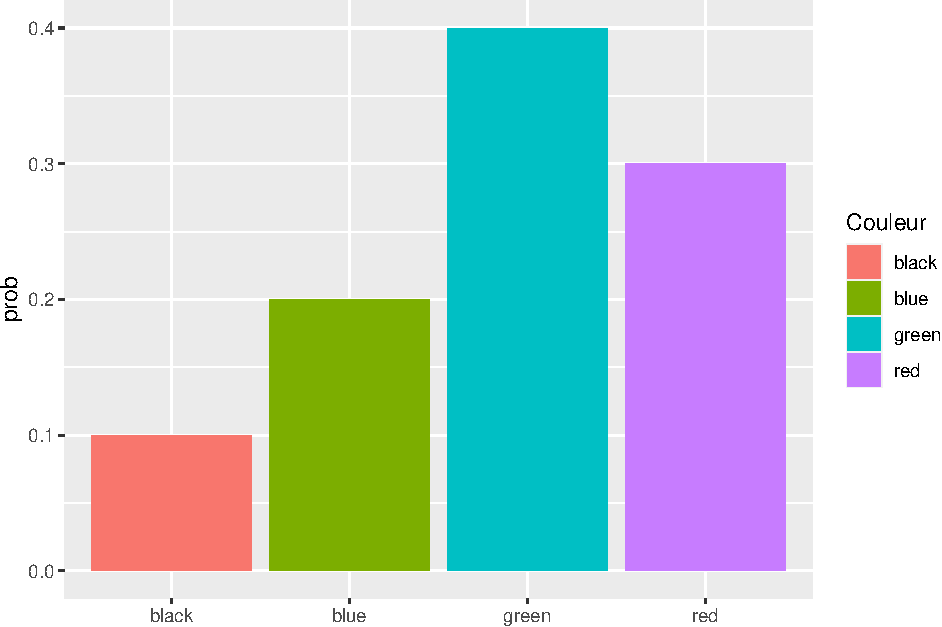
\includegraphics{TUTO_VISU_files/figure-latex/unnamed-chunk-31-1} \end{center}

\BeginKnitrBlock{exercise}[Lissage]
\protect\hypertarget{exr:exo-stat2}{}{\label{exr:exo-stat2} \iffalse (Lissage) \fi{} }
\EndKnitrBlock{exercise}

\begin{enumerate}
\def\labelenumi{\arabic{enumi}.}
\tightlist
\item
  Représenter le lissage non linéaire de la variable \texttt{price} contre la variable \texttt{carat} à l'aide de \texttt{geom\_smooth} puis de \texttt{stat\_smooth}.
\item
  Même question mais avec une ligne en pointillés à la place d'un trait plein.
\end{enumerate}

\begin{Shaded}
\begin{Highlighting}[]
\OperatorTok{>}\StringTok{ }\KeywordTok{ggplot}\NormalTok{(diamonds2)}\OperatorTok{+}\KeywordTok{aes}\NormalTok{(}\DataTypeTok{x=}\NormalTok{carat,}\DataTypeTok{y=}\NormalTok{price)}\OperatorTok{+}\KeywordTok{geom_smooth}\NormalTok{(}\DataTypeTok{method=}\StringTok{"loess"}\NormalTok{)}
\end{Highlighting}
\end{Shaded}

\begin{center}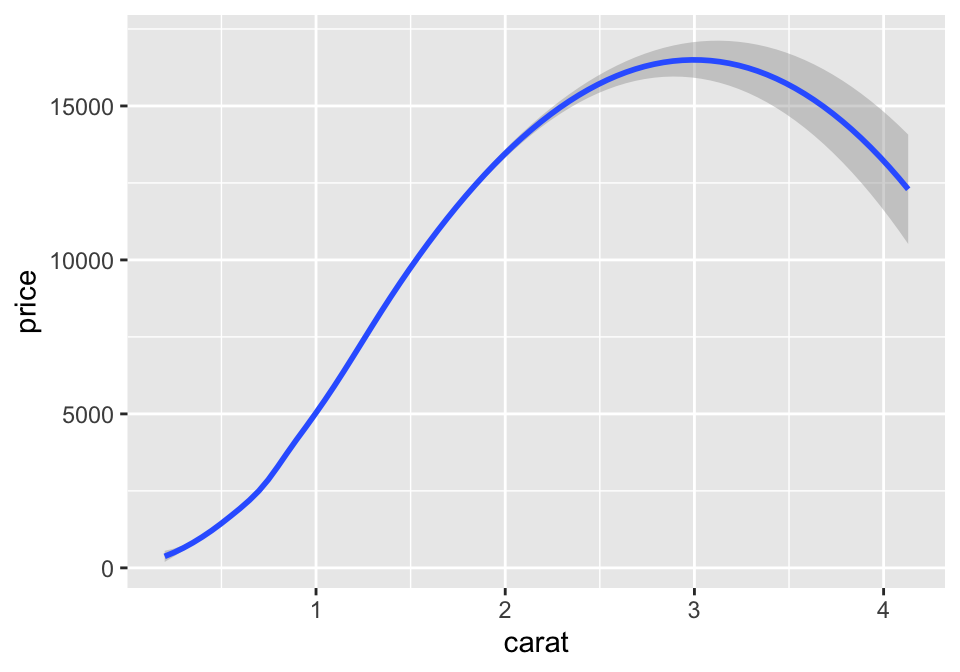
\includegraphics{TUTO_VISU_files/figure-latex/unnamed-chunk-32-1} \end{center}

\begin{Shaded}
\begin{Highlighting}[]
\OperatorTok{>}\StringTok{ }\KeywordTok{ggplot}\NormalTok{(diamonds2)}\OperatorTok{+}\KeywordTok{aes}\NormalTok{(}\DataTypeTok{x=}\NormalTok{carat,}\DataTypeTok{y=}\NormalTok{price)}\OperatorTok{+}\KeywordTok{stat_smooth}\NormalTok{(}\DataTypeTok{method=}\StringTok{"loess"}\NormalTok{)}
\end{Highlighting}
\end{Shaded}

\begin{center}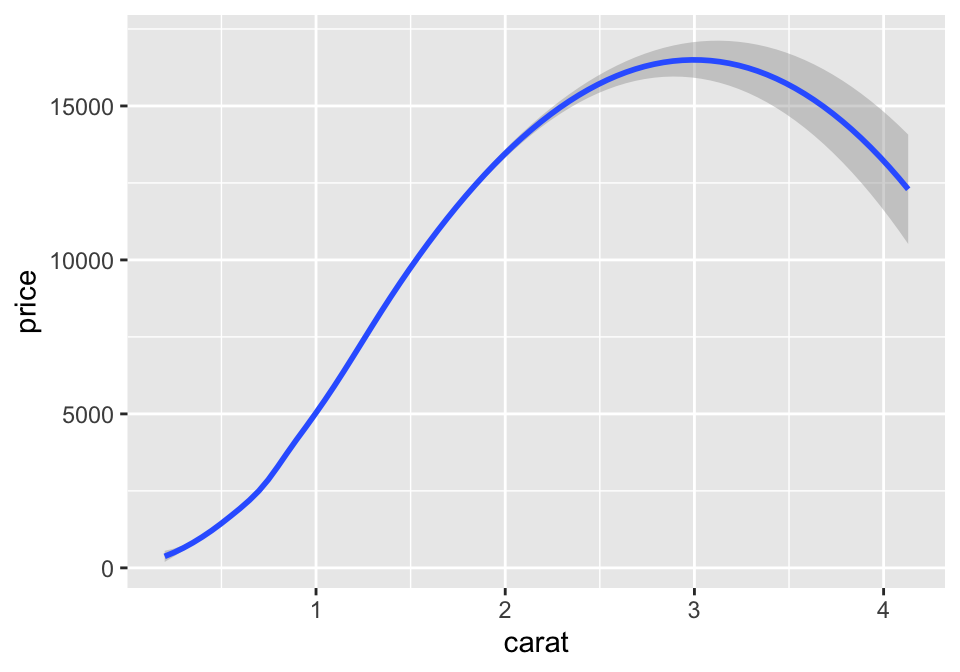
\includegraphics{TUTO_VISU_files/figure-latex/unnamed-chunk-32-2} \end{center}

\begin{Shaded}
\begin{Highlighting}[]
\OperatorTok{>}\StringTok{ }\KeywordTok{ggplot}\NormalTok{(diamonds2)}\OperatorTok{+}\KeywordTok{aes}\NormalTok{(}\DataTypeTok{x=}\NormalTok{carat,}\DataTypeTok{y=}\NormalTok{price)}\OperatorTok{+}\KeywordTok{geom_smooth}\NormalTok{(}\DataTypeTok{method=}\StringTok{"loess"}\NormalTok{,}\DataTypeTok{linetype=}\StringTok{"dotted"}\NormalTok{)}
\end{Highlighting}
\end{Shaded}

\begin{center}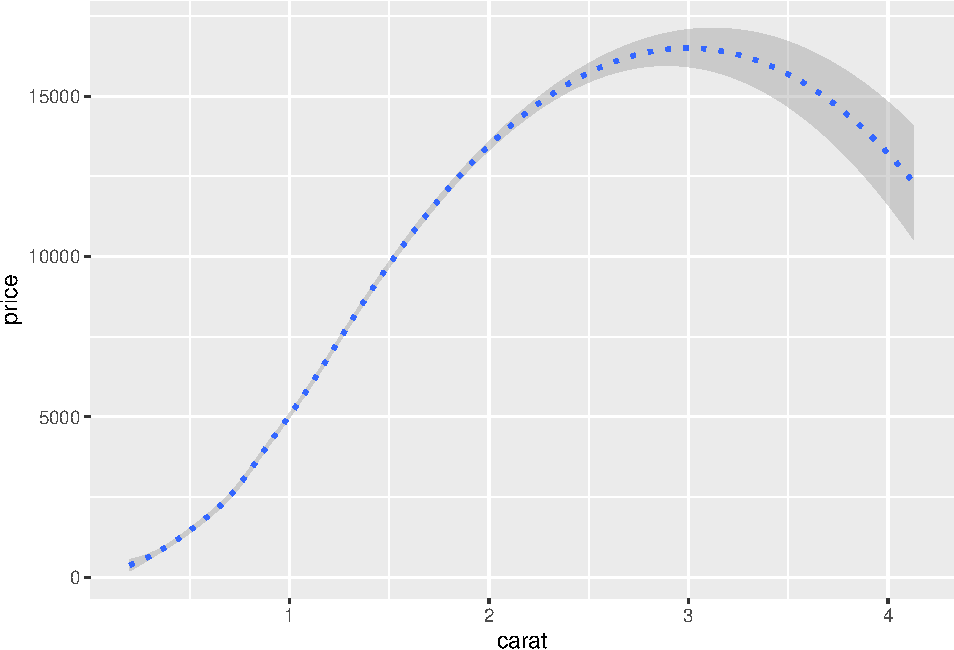
\includegraphics{TUTO_VISU_files/figure-latex/unnamed-chunk-32-3} \end{center}

\begin{Shaded}
\begin{Highlighting}[]
\OperatorTok{>}\StringTok{ }\KeywordTok{ggplot}\NormalTok{(diamonds2)}\OperatorTok{+}\KeywordTok{aes}\NormalTok{(}\DataTypeTok{x=}\NormalTok{carat,}\DataTypeTok{y=}\NormalTok{price)}\OperatorTok{+}\KeywordTok{stat_smooth}\NormalTok{(}\DataTypeTok{method=}\StringTok{"loess"}\NormalTok{,}\DataTypeTok{geom=}\StringTok{"point"}\NormalTok{)}
\end{Highlighting}
\end{Shaded}

\begin{center}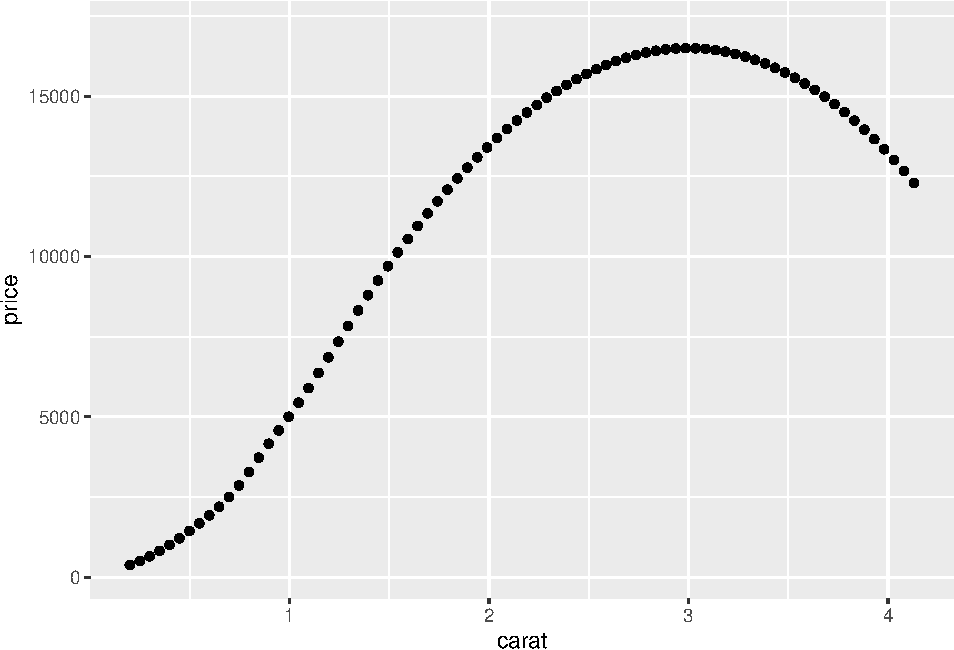
\includegraphics{TUTO_VISU_files/figure-latex/unnamed-chunk-32-4} \end{center}

\hypertarget{scales}{%
\subsection{\texorpdfstring{\texttt{Scales}}{Scales}}\label{scales}}

Les échelles (\textbf{scales}) controlent tout un tas d'options telles que des changements de couleurs, d'échelles ou de limites d'axes, de symboles, etc\ldots{} L'utilisation n'est pas simple et nécessite de la pratique. On utilise généralement ce verbe à la dernière étape de construction du graphe. La syntaxe est définie comme suit :

\begin{itemize}
\tightlist
\item
  début : \texttt{scale\_}.
\item
  ajout de l'aesthetics que l'on souhaite modifier (\texttt{color}, \texttt{fill}, \texttt{x\_}).
\item
  fin : nom de l'échelle (\texttt{manual}, \texttt{identity}\ldots{})
\end{itemize}

Par exemple,

\begin{Shaded}
\begin{Highlighting}[]
\OperatorTok{>}\StringTok{ }\KeywordTok{ggplot}\NormalTok{(diamonds2)}\OperatorTok{+}\KeywordTok{aes}\NormalTok{(}\DataTypeTok{x=}\NormalTok{carat,}\DataTypeTok{y=}\NormalTok{price,}\DataTypeTok{color=}\NormalTok{cut)}\OperatorTok{+}\KeywordTok{geom_point}\NormalTok{()}\OperatorTok{+}
\OperatorTok{+}\StringTok{   }\KeywordTok{scale_color_manual}\NormalTok{(}\DataTypeTok{values=}\KeywordTok{c}\NormalTok{(}\StringTok{"Fair"}\NormalTok{=}\StringTok{"black"}\NormalTok{,}\StringTok{"Good"}\NormalTok{=}\StringTok{"yellow"}\NormalTok{,}
\OperatorTok{+}\StringTok{                               "Very Good"}\NormalTok{=}\StringTok{"blue"}\NormalTok{,}\StringTok{"Premium"}\NormalTok{=}\StringTok{"red"}\NormalTok{,}\StringTok{"Ideal"}\NormalTok{=}\StringTok{"green"}\NormalTok{))}
\end{Highlighting}
\end{Shaded}

\begin{center}
\includegraphics{TUTO_VISU_files/figure-latex/unnamed-chunk-33-1} \end{center}

Voici quelques exemples des principales échelles :

\begin{longtable}[]{@{}lll@{}}
\caption{\label{tab:scales} Exemples d'échelles}\tabularnewline
\toprule
aes & Discret & Continu\tabularnewline
\midrule
\endfirsthead
\toprule
aes & Discret & Continu\tabularnewline
\midrule
\endhead
Couleur (color et fill) & brewer & gradient\tabularnewline
- & grey & gradient2\tabularnewline
- & hue & gradientn\tabularnewline
- & identity &\tabularnewline
- & manual &\tabularnewline
Position (x et y) & discrete & continous\tabularnewline
- & & date\tabularnewline
Forme & shape &\tabularnewline
- & identity &\tabularnewline
- & manual &\tabularnewline
Taille & identity & size\tabularnewline
- & manual &\tabularnewline
\bottomrule
\end{longtable}

Nous présentons quelques exemples d'utilisation des échelles :

\begin{itemize}
\tightlist
\item
  \texttt{Couleur\ dans\ un\ diagramme\ en\ barres}
\end{itemize}

\begin{Shaded}
\begin{Highlighting}[]
\OperatorTok{>}\StringTok{ }\NormalTok{p1 <-}\StringTok{ }\KeywordTok{ggplot}\NormalTok{(diamonds2)}\OperatorTok{+}\KeywordTok{aes}\NormalTok{(}\DataTypeTok{x=}\NormalTok{cut)}\OperatorTok{+}\KeywordTok{geom_bar}\NormalTok{(}\KeywordTok{aes}\NormalTok{(}\DataTypeTok{fill=}\NormalTok{cut))}
\OperatorTok{>}\StringTok{ }\NormalTok{p1}
\end{Highlighting}
\end{Shaded}

\begin{center}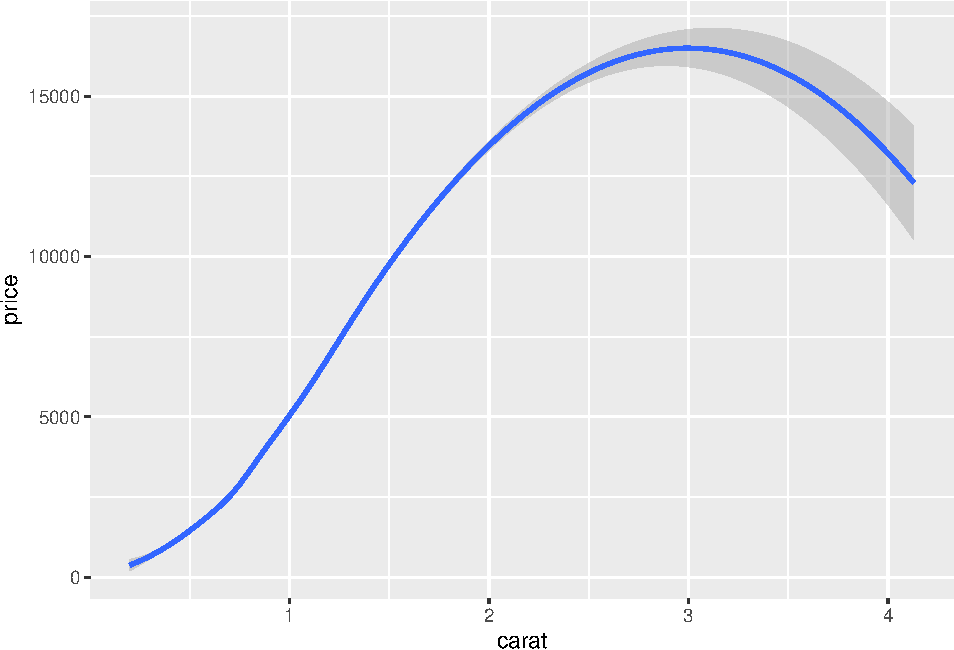
\includegraphics{TUTO_VISU_files/figure-latex/unnamed-chunk-34-1} \end{center}

On change la couleur en utilisant la palette \textbf{Purples} :

\begin{Shaded}
\begin{Highlighting}[]
\OperatorTok{>}\StringTok{ }\NormalTok{p1}\OperatorTok{+}\KeywordTok{scale_fill_brewer}\NormalTok{(}\DataTypeTok{palette=}\StringTok{"Purples"}\NormalTok{)}
\end{Highlighting}
\end{Shaded}

\begin{center}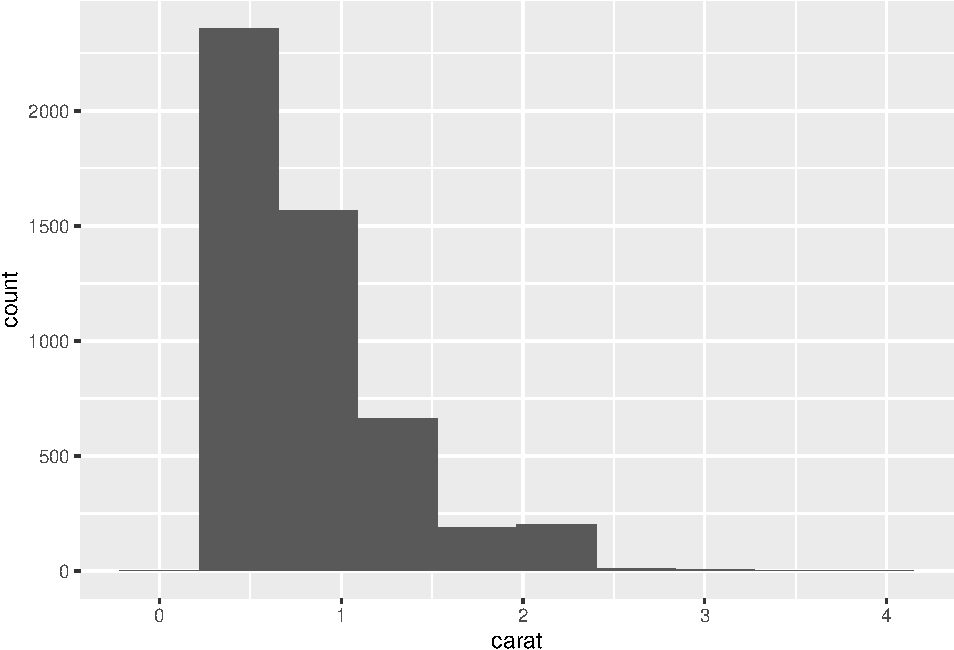
\includegraphics{TUTO_VISU_files/figure-latex/unnamed-chunk-35-1} \end{center}

\begin{itemize}
\tightlist
\item
  \texttt{Gradient\ de\ couleurs\ pour\ un\ nuage\ de\ points} :
\end{itemize}

\begin{Shaded}
\begin{Highlighting}[]
\OperatorTok{>}\StringTok{ }\NormalTok{p2 <-}\StringTok{ }\KeywordTok{ggplot}\NormalTok{(diamonds2)}\OperatorTok{+}\KeywordTok{aes}\NormalTok{(}\DataTypeTok{x=}\NormalTok{carat,}\DataTypeTok{y=}\NormalTok{price)}\OperatorTok{+}\KeywordTok{geom_point}\NormalTok{(}\KeywordTok{aes}\NormalTok{(}\DataTypeTok{color=}\NormalTok{depth))}
\OperatorTok{>}\StringTok{ }\NormalTok{p2}
\end{Highlighting}
\end{Shaded}

\begin{center}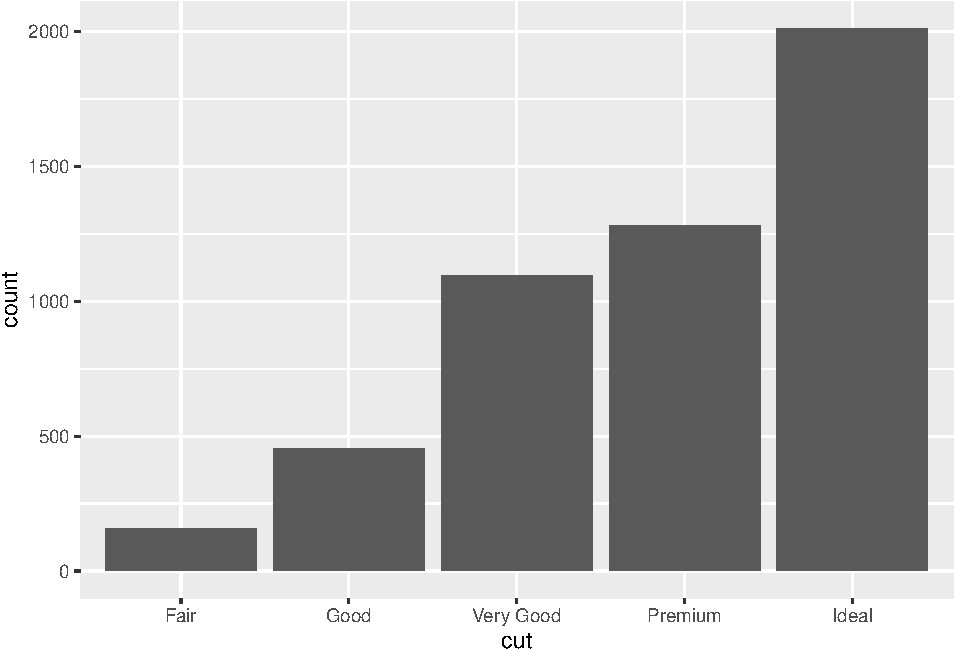
\includegraphics{TUTO_VISU_files/figure-latex/unnamed-chunk-36-1} \end{center}

On change le gradient de couleur

\begin{Shaded}
\begin{Highlighting}[]
\OperatorTok{>}\StringTok{ }\NormalTok{p2}\OperatorTok{+}\KeywordTok{scale_color_gradient}\NormalTok{(}\DataTypeTok{low=}\StringTok{"red"}\NormalTok{,}\DataTypeTok{high=}\StringTok{"yellow"}\NormalTok{)}
\end{Highlighting}
\end{Shaded}

\begin{center}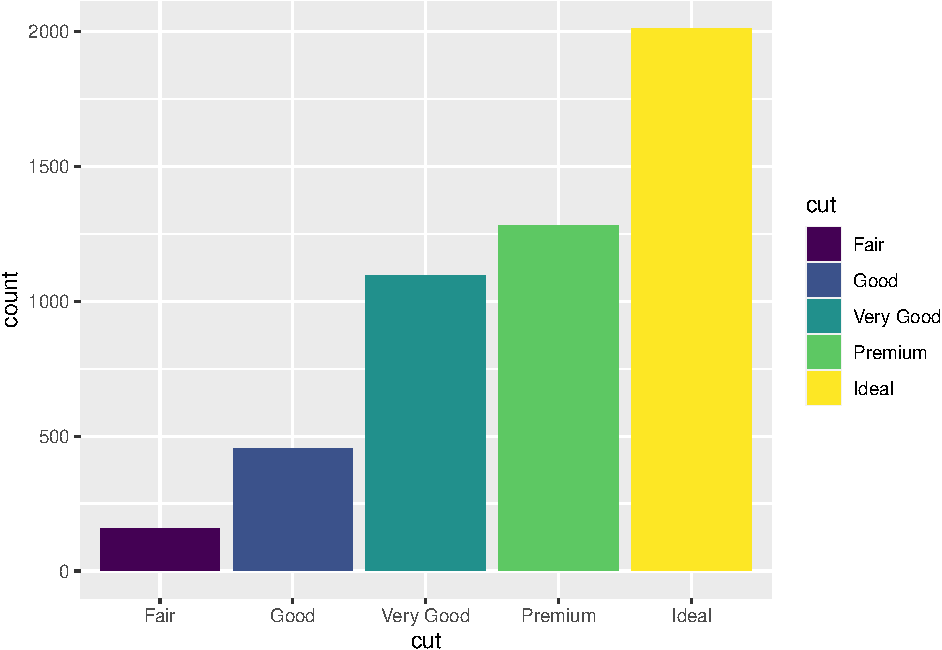
\includegraphics{TUTO_VISU_files/figure-latex/unnamed-chunk-37-1} \end{center}

\begin{itemize}
\tightlist
\item
  \texttt{Modification\ sur\ les\ axes}
\end{itemize}

\begin{Shaded}
\begin{Highlighting}[]
\OperatorTok{>}\StringTok{ }\NormalTok{p2}\OperatorTok{+}\KeywordTok{scale_x_continuous}\NormalTok{(}\DataTypeTok{breaks=}\KeywordTok{seq}\NormalTok{(}\FloatTok{0.5}\NormalTok{,}\DecValTok{3}\NormalTok{,}\DataTypeTok{by=}\FloatTok{0.5}\NormalTok{))}\OperatorTok{+}
\OperatorTok{+}\StringTok{   }\KeywordTok{scale_y_continuous}\NormalTok{(}\DataTypeTok{name=}\StringTok{"prix"}\NormalTok{)}\OperatorTok{+}
\OperatorTok{+}\StringTok{   }\KeywordTok{scale_color_gradient}\NormalTok{(}\StringTok{"Profondeur"}\NormalTok{)}
\end{Highlighting}
\end{Shaded}

\begin{center}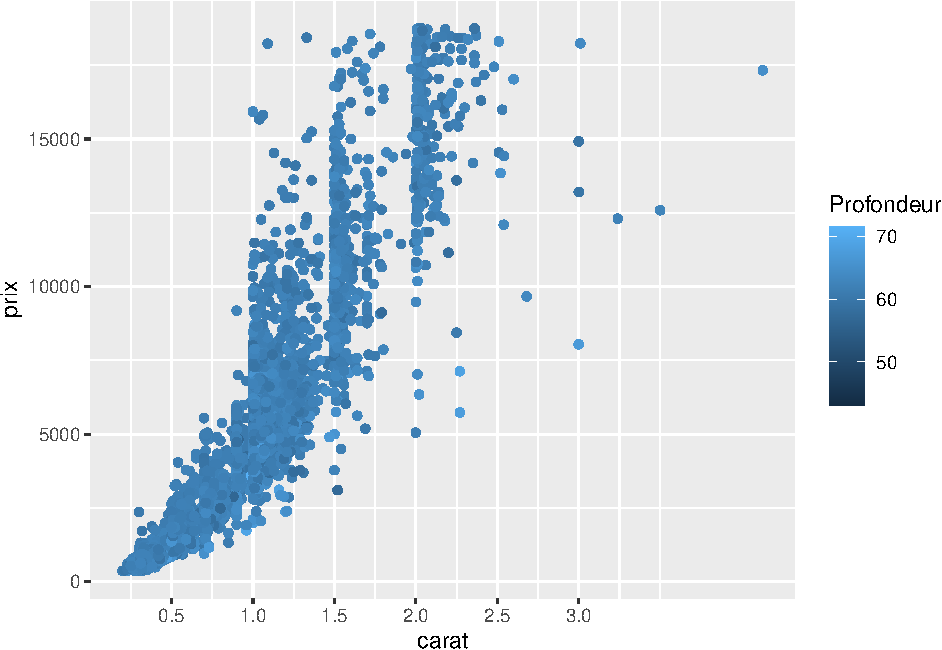
\includegraphics{TUTO_VISU_files/figure-latex/unnamed-chunk-38-1} \end{center}

\hypertarget{group-et-facets}{%
\subsection{\texorpdfstring{\texttt{Group\ et\ facets}}{Group et facets}}\label{group-et-facets}}

\textbf{ggplot} permet de faire des représentations pour des groupes d'individus. On procède généralement de deux façons différentes :

\begin{itemize}
\tightlist
\item
  visualisation de sous groupes sur le même graphe, on utilise l'option \emph{group} dans \textbf{aes} ;
\item
  visualisation de sous groupes sur des graphes différents, on utilise le verbe \textbf{facets}.
\end{itemize}

Représentons ici (sur le même graphe) le lisseur \textbf{price vs carat} pour chaque modalité de \emph{cut}

\begin{Shaded}
\begin{Highlighting}[]
\OperatorTok{>}\StringTok{ }\KeywordTok{ggplot}\NormalTok{(diamonds2)}\OperatorTok{+}\KeywordTok{aes}\NormalTok{(}\DataTypeTok{x=}\NormalTok{carat,}\DataTypeTok{y=}\NormalTok{price,}\DataTypeTok{group=}\NormalTok{cut)}\OperatorTok{+}
\OperatorTok{+}\StringTok{   }\KeywordTok{geom_smooth}\NormalTok{(}\DataTypeTok{method=}\StringTok{"loess"}\NormalTok{)}
\end{Highlighting}
\end{Shaded}

\begin{center}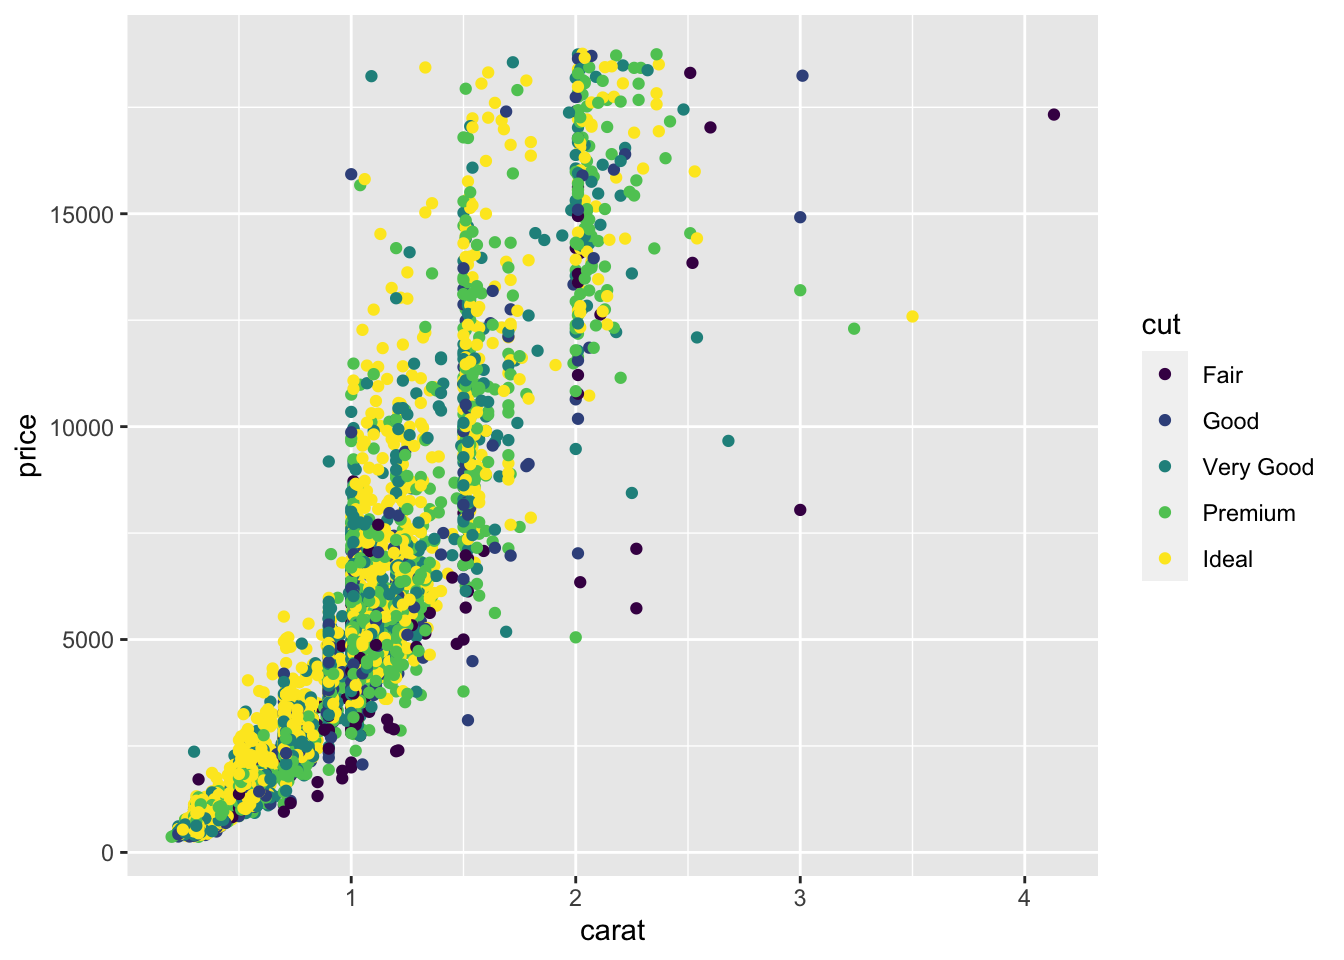
\includegraphics{TUTO_VISU_files/figure-latex/unnamed-chunk-39-1} \end{center}

Pour obtenir cette représentation sur plusieurs fenêtres, on utilise

\begin{Shaded}
\begin{Highlighting}[]
\OperatorTok{>}\StringTok{ }\KeywordTok{ggplot}\NormalTok{(diamonds2)}\OperatorTok{+}\KeywordTok{aes}\NormalTok{(}\DataTypeTok{x=}\NormalTok{carat,}\DataTypeTok{y=}\NormalTok{price)}\OperatorTok{+}
\OperatorTok{+}\StringTok{   }\KeywordTok{geom_smooth}\NormalTok{(}\DataTypeTok{method=}\StringTok{"loess"}\NormalTok{)}\OperatorTok{+}\KeywordTok{facet_wrap}\NormalTok{(}\OperatorTok{~}\NormalTok{cut)}
\end{Highlighting}
\end{Shaded}

\begin{center}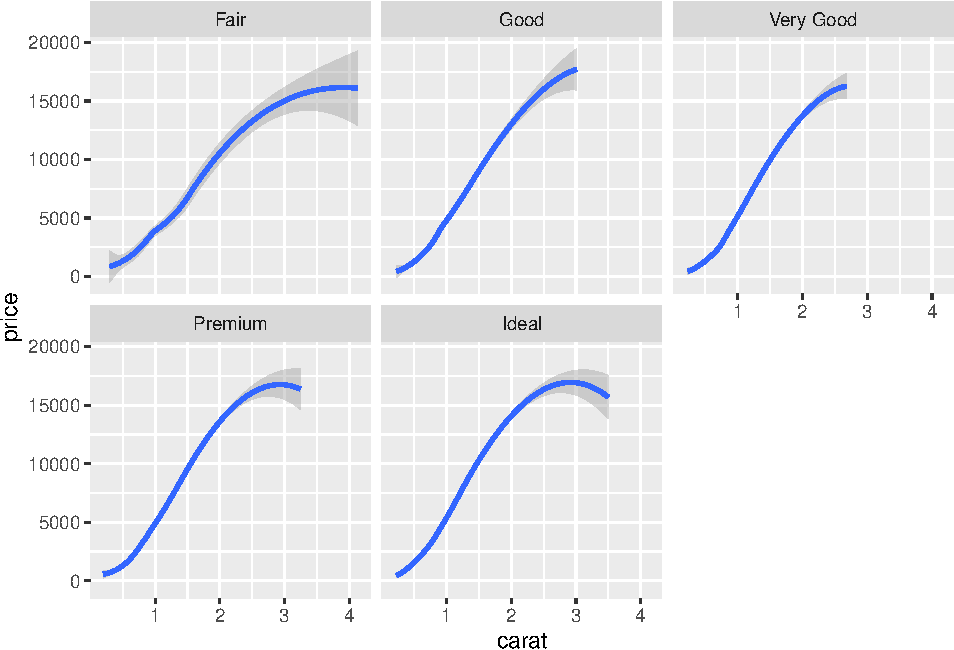
\includegraphics{TUTO_VISU_files/figure-latex/unnamed-chunk-40-1} \end{center}

\begin{Shaded}
\begin{Highlighting}[]
\OperatorTok{>}\StringTok{ }\KeywordTok{ggplot}\NormalTok{(diamonds2)}\OperatorTok{+}\KeywordTok{aes}\NormalTok{(}\DataTypeTok{x=}\NormalTok{carat,}\DataTypeTok{y=}\NormalTok{price)}\OperatorTok{+}
\OperatorTok{+}\StringTok{   }\KeywordTok{geom_smooth}\NormalTok{(}\DataTypeTok{method=}\StringTok{"loess"}\NormalTok{)}\OperatorTok{+}\KeywordTok{facet_wrap}\NormalTok{(}\OperatorTok{~}\NormalTok{cut,}\DataTypeTok{nrow=}\DecValTok{1}\NormalTok{)}
\end{Highlighting}
\end{Shaded}

\begin{center}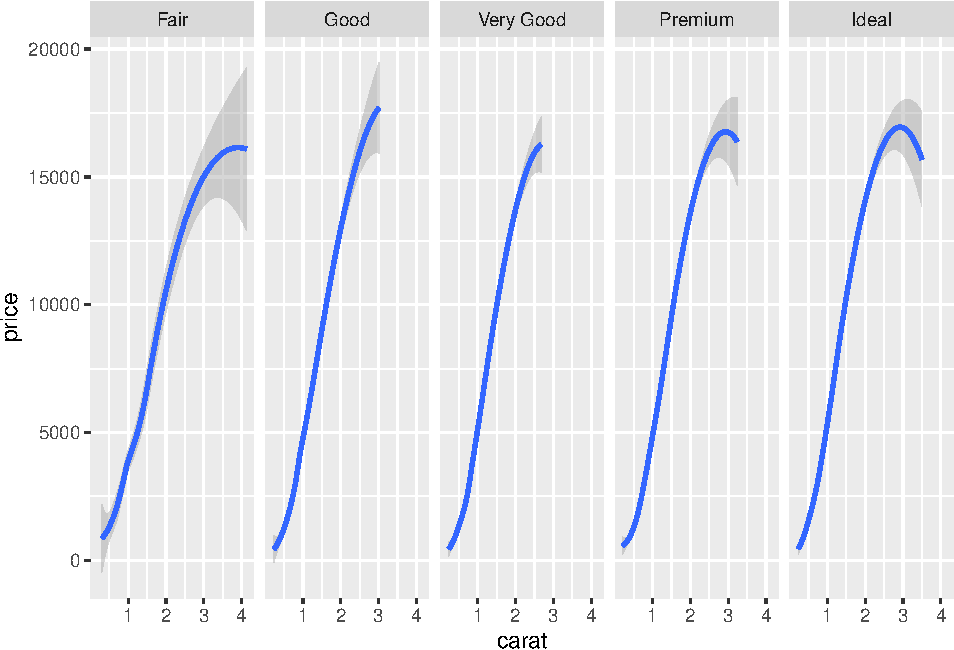
\includegraphics{TUTO_VISU_files/figure-latex/unnamed-chunk-40-2} \end{center}

\emph{facet\_grid} et \emph{facet\_wrap} font des choses proches mais divisent la fenêtre de façon différente :

\begin{Shaded}
\begin{Highlighting}[]
\OperatorTok{>}\StringTok{ }\KeywordTok{ggplot}\NormalTok{(diamonds2)}\OperatorTok{+}\KeywordTok{aes}\NormalTok{(}\DataTypeTok{x=}\NormalTok{carat,}\DataTypeTok{y=}\NormalTok{price)}\OperatorTok{+}\KeywordTok{geom_point}\NormalTok{()}\OperatorTok{+}
\OperatorTok{+}\StringTok{   }\KeywordTok{geom_smooth}\NormalTok{(}\DataTypeTok{method=}\StringTok{"lm"}\NormalTok{)}\OperatorTok{+}\KeywordTok{facet_grid}\NormalTok{(color}\OperatorTok{~}\NormalTok{cut)}
\end{Highlighting}
\end{Shaded}

\begin{center}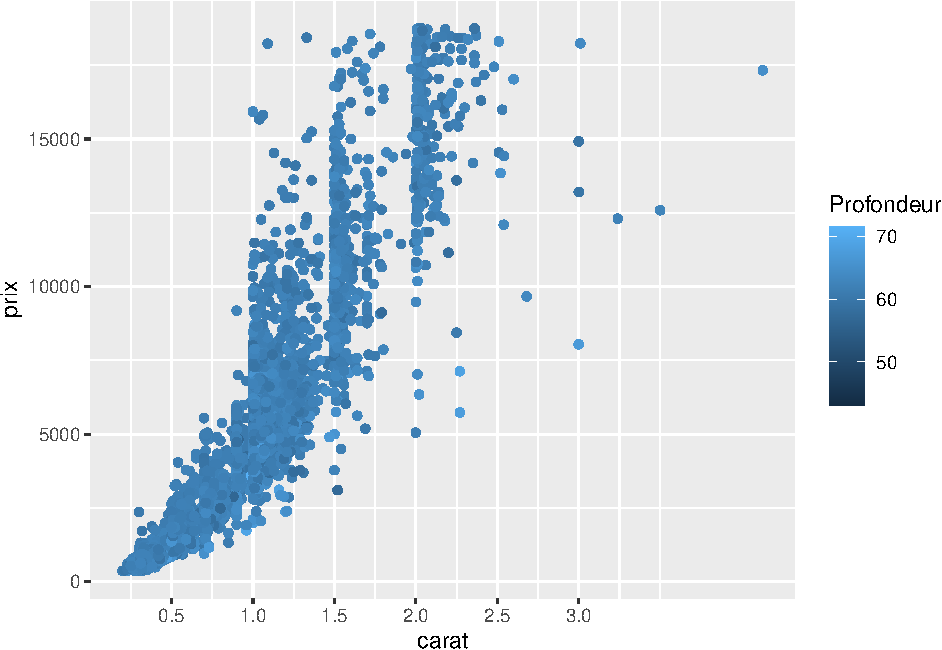
\includegraphics{TUTO_VISU_files/figure-latex/unnamed-chunk-41-1} \end{center}

\begin{Shaded}
\begin{Highlighting}[]
\OperatorTok{>}\StringTok{ }\KeywordTok{ggplot}\NormalTok{(diamonds2)}\OperatorTok{+}\KeywordTok{aes}\NormalTok{(}\DataTypeTok{x=}\NormalTok{carat,}\DataTypeTok{y=}\NormalTok{price)}\OperatorTok{+}\KeywordTok{geom_point}\NormalTok{()}\OperatorTok{+}
\OperatorTok{+}\StringTok{   }\KeywordTok{geom_smooth}\NormalTok{(}\DataTypeTok{method=}\StringTok{"lm"}\NormalTok{)}\OperatorTok{+}\KeywordTok{facet_wrap}\NormalTok{(color}\OperatorTok{~}\NormalTok{cut)}
\end{Highlighting}
\end{Shaded}

\begin{center}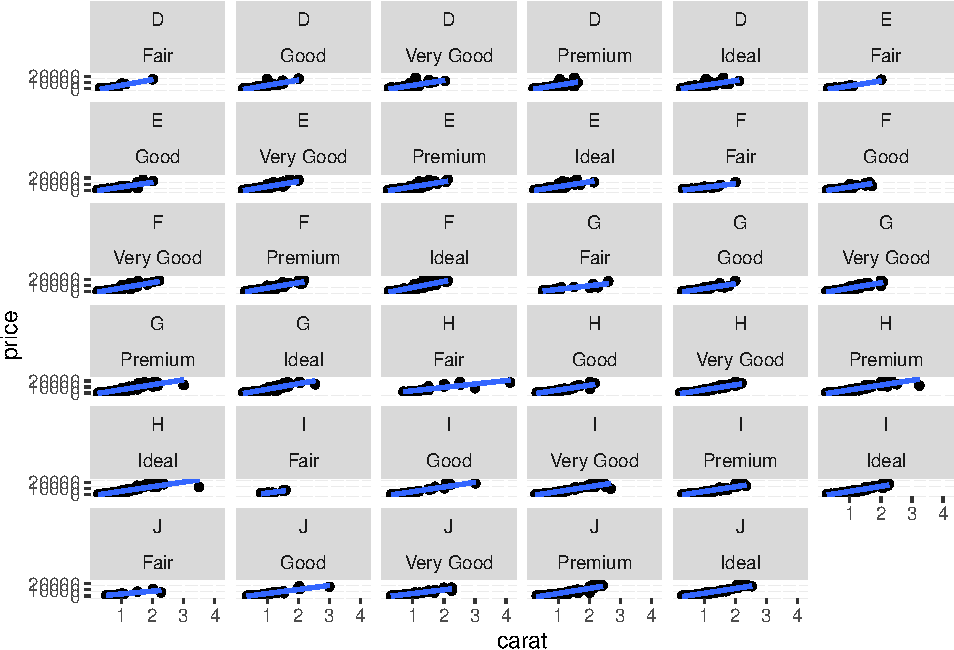
\includegraphics{TUTO_VISU_files/figure-latex/unnamed-chunk-41-2} \end{center}

\hypertarget{compluxe9ments}{%
\section{Compléments}\label{compluxe9ments}}

La syntaxe \textbf{ggplot} est définie selon le schéma :

\begin{Shaded}
\begin{Highlighting}[]
\OperatorTok{>}\StringTok{ }\KeywordTok{ggplot}\NormalTok{()}\OperatorTok{+}\KeywordTok{aes}\NormalTok{()}\OperatorTok{+}\KeywordTok{geom_}\NormalTok{()}\OperatorTok{+}\KeywordTok{scale_}\NormalTok{()}
\end{Highlighting}
\end{Shaded}

Elle est très flexible, on peut par exemple spécifier les variables de \texttt{aes} dans les verbes \texttt{ggplot} ou \texttt{geom\_} :

\begin{Shaded}
\begin{Highlighting}[]
\OperatorTok{>}\StringTok{ }\KeywordTok{ggplot}\NormalTok{(diamonds2)}\OperatorTok{+}\KeywordTok{aes}\NormalTok{(}\DataTypeTok{x=}\NormalTok{carat,}\DataTypeTok{y=}\NormalTok{price)}\OperatorTok{+}\KeywordTok{geom_point}\NormalTok{()}
\end{Highlighting}
\end{Shaded}

\begin{center}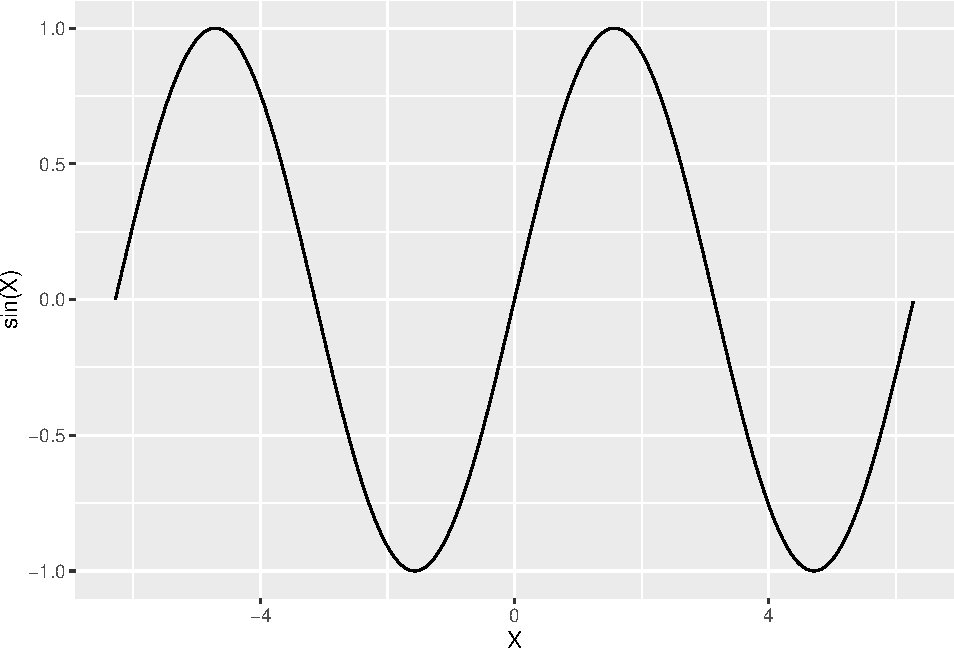
\includegraphics{TUTO_VISU_files/figure-latex/unnamed-chunk-43-1} \end{center}

\begin{Shaded}
\begin{Highlighting}[]
\OperatorTok{>}\StringTok{ }\KeywordTok{ggplot}\NormalTok{(diamonds2,}\KeywordTok{aes}\NormalTok{(}\DataTypeTok{x=}\NormalTok{carat,}\DataTypeTok{y=}\NormalTok{price))}\OperatorTok{+}\KeywordTok{geom_point}\NormalTok{()}
\end{Highlighting}
\end{Shaded}

\begin{center}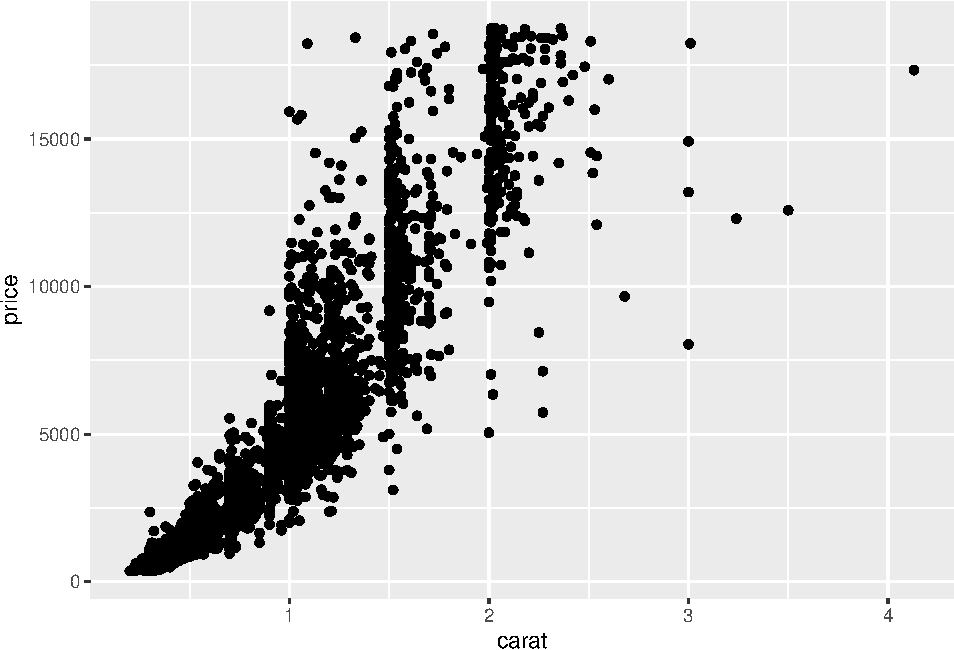
\includegraphics{TUTO_VISU_files/figure-latex/unnamed-chunk-43-2} \end{center}

\begin{Shaded}
\begin{Highlighting}[]
\OperatorTok{>}\StringTok{ }\KeywordTok{ggplot}\NormalTok{(diamonds2)}\OperatorTok{+}\KeywordTok{geom_point}\NormalTok{(}\KeywordTok{aes}\NormalTok{(}\DataTypeTok{x=}\NormalTok{carat,}\DataTypeTok{y=}\NormalTok{price))}
\end{Highlighting}
\end{Shaded}

\begin{center}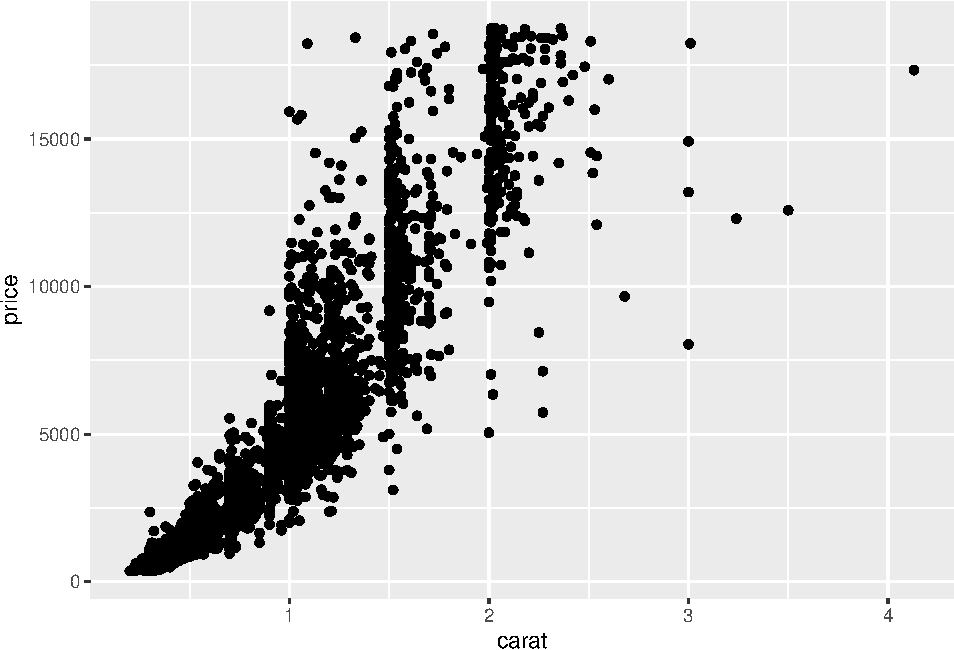
\includegraphics{TUTO_VISU_files/figure-latex/unnamed-chunk-43-3} \end{center}

Ceci peut se révéler très utile lorsqu'on utilise des \textbf{aes} différents dans les \textbf{geom\_}.

On peut aussi construire un graphe à l'aide de différents jeux de données :

\begin{Shaded}
\begin{Highlighting}[]
\OperatorTok{>}\StringTok{ }\NormalTok{X <-}\StringTok{ }\KeywordTok{seq}\NormalTok{(}\OperatorTok{-}\DecValTok{2}\OperatorTok{*}\NormalTok{pi,}\DecValTok{2}\OperatorTok{*}\NormalTok{pi,}\DataTypeTok{by=}\FloatTok{0.001}\NormalTok{)}
\OperatorTok{>}\StringTok{ }\NormalTok{Y1 <-}\StringTok{ }\KeywordTok{cos}\NormalTok{(X)}
\OperatorTok{>}\StringTok{ }\NormalTok{Y2 <-}\StringTok{ }\KeywordTok{sin}\NormalTok{(X)}
\OperatorTok{>}\StringTok{ }\NormalTok{donnees1 <-}\StringTok{ }\KeywordTok{data.frame}\NormalTok{(X,Y1)}
\OperatorTok{>}\StringTok{ }\NormalTok{donnees2 <-}\StringTok{ }\KeywordTok{data.frame}\NormalTok{(X,Y2)}
\OperatorTok{>}\StringTok{ }\KeywordTok{ggplot}\NormalTok{(donnees1)}\OperatorTok{+}\KeywordTok{geom_line}\NormalTok{(}\KeywordTok{aes}\NormalTok{(}\DataTypeTok{x=}\NormalTok{X,}\DataTypeTok{y=}\NormalTok{Y1))}\OperatorTok{+}
\OperatorTok{+}\StringTok{   }\KeywordTok{geom_line}\NormalTok{(}\DataTypeTok{data=}\NormalTok{donnees2,}\KeywordTok{aes}\NormalTok{(}\DataTypeTok{x=}\NormalTok{X,}\DataTypeTok{y=}\NormalTok{Y2),}\DataTypeTok{color=}\StringTok{"red"}\NormalTok{)}
\end{Highlighting}
\end{Shaded}

\begin{center}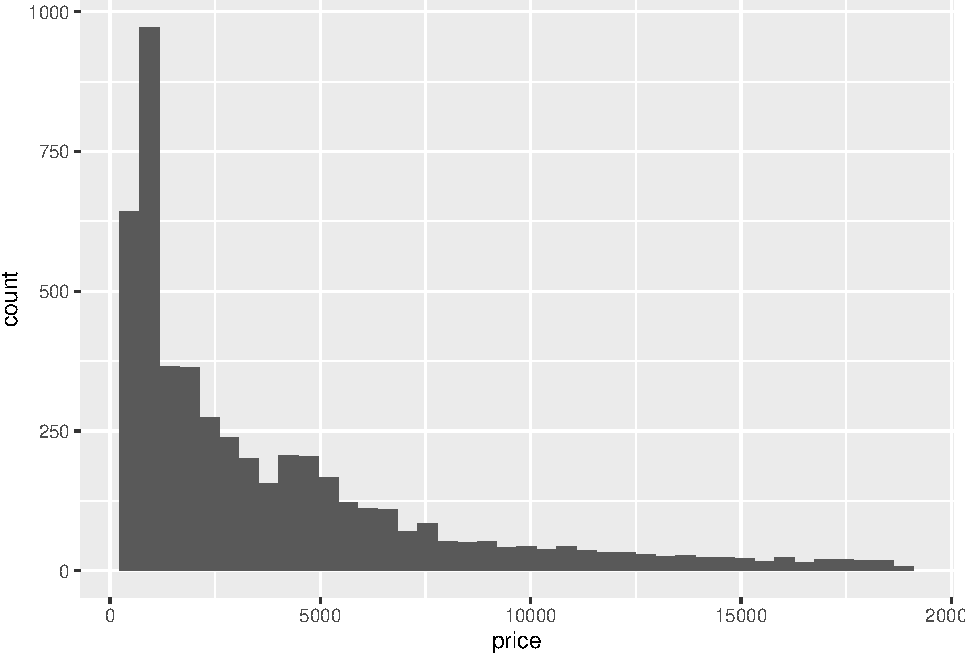
\includegraphics{TUTO_VISU_files/figure-latex/unnamed-chunk-44-1} \end{center}

Il existe d'autres fonctions \textbf{ggplot} :

\begin{itemize}
\tightlist
\item
  \textbf{ggtitle} pour ajouter un titre.
\item
  \textbf{ggsave} pour sauver un graphe.
\item
  \textbf{theme\_} pour changer le theme du graphe.
\end{itemize}

\begin{Shaded}
\begin{Highlighting}[]
\OperatorTok{>}\StringTok{ }\NormalTok{p <-}\StringTok{ }\KeywordTok{ggplot}\NormalTok{(diamonds2)}\OperatorTok{+}\KeywordTok{aes}\NormalTok{(}\DataTypeTok{x=}\NormalTok{carat,}\DataTypeTok{y=}\NormalTok{price,}\DataTypeTok{color=}\NormalTok{cut)}\OperatorTok{+}\KeywordTok{geom_point}\NormalTok{()}
\OperatorTok{>}\StringTok{ }\NormalTok{p}\OperatorTok{+}\KeywordTok{theme_bw}\NormalTok{()}
\end{Highlighting}
\end{Shaded}

\begin{center}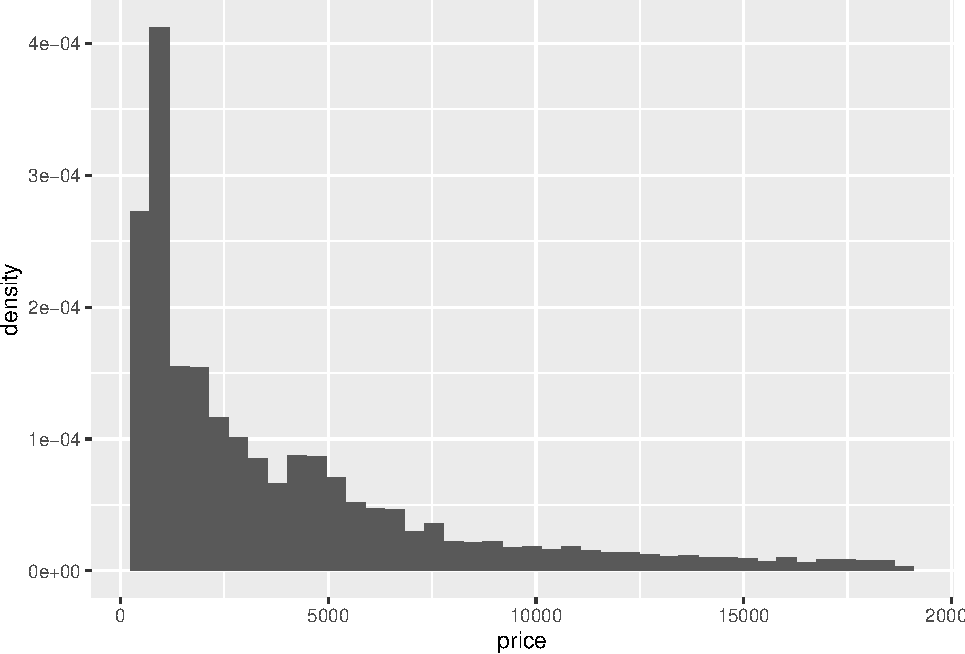
\includegraphics{TUTO_VISU_files/figure-latex/unnamed-chunk-45-1} \end{center}

\begin{Shaded}
\begin{Highlighting}[]
\OperatorTok{>}\StringTok{ }\NormalTok{p}\OperatorTok{+}\KeywordTok{theme_classic}\NormalTok{()}
\end{Highlighting}
\end{Shaded}

\begin{center}\includegraphics{TUTO_VISU_files/figure-latex/unnamed-chunk-45-2} \end{center}

\begin{Shaded}
\begin{Highlighting}[]
\OperatorTok{>}\StringTok{ }\NormalTok{p}\OperatorTok{+}\KeywordTok{theme_grey}\NormalTok{()}
\end{Highlighting}
\end{Shaded}

\begin{center}\includegraphics{TUTO_VISU_files/figure-latex/unnamed-chunk-45-3} \end{center}

\begin{Shaded}
\begin{Highlighting}[]
\OperatorTok{>}\StringTok{ }\NormalTok{p}\OperatorTok{+}\KeywordTok{theme_bw}\NormalTok{()}
\end{Highlighting}
\end{Shaded}

\begin{center}\includegraphics{TUTO_VISU_files/figure-latex/unnamed-chunk-45-4} \end{center}

D'autres thèmes sont disponibles dans le package \textbf{ggtheme}. On pourra également parler de la fonction \texttt{set\_theme} qui permet de préciser modifier le thème par défaut pour un document \textbf{Markdown}.

\hypertarget{quelques-exercices-suppluxe9mentaires}{%
\section{Quelques exercices supplémentaires}\label{quelques-exercices-suppluxe9mentaires}}

\BeginKnitrBlock{exercise}[Fonctions cosinus et sinus]
\protect\hypertarget{exr:exo-cos-sin}{}{\label{exr:exo-cos-sin} \iffalse (Fonctions cosinus et sinus) \fi{} }
\EndKnitrBlock{exercise}

\begin{enumerate}
\def\labelenumi{\arabic{enumi}.}
\tightlist
\item
  Tracer les fonctions sinus et cosinus. On utilisera tout d'abord deux jeux de données : un pour le sinus, l'autre pour le cosinus.
\end{enumerate}

\begin{Shaded}
\begin{Highlighting}[]
\OperatorTok{>}\StringTok{ }\NormalTok{X <-}\StringTok{ }\KeywordTok{seq}\NormalTok{(}\OperatorTok{-}\DecValTok{2}\OperatorTok{*}\NormalTok{pi,}\DecValTok{2}\OperatorTok{*}\NormalTok{pi,}\DataTypeTok{by=}\FloatTok{0.001}\NormalTok{)}
\OperatorTok{>}\StringTok{ }\NormalTok{Y1 <-}\StringTok{ }\KeywordTok{cos}\NormalTok{(X)}
\OperatorTok{>}\StringTok{ }\NormalTok{Y2 <-}\StringTok{ }\KeywordTok{sin}\NormalTok{(X)}
\OperatorTok{>}\StringTok{ }\NormalTok{donnees1 <-}\StringTok{ }\KeywordTok{data.frame}\NormalTok{(X,Y1)}
\OperatorTok{>}\StringTok{ }\NormalTok{donnees2 <-}\StringTok{ }\KeywordTok{data.frame}\NormalTok{(X,Y2)}
\OperatorTok{>}\StringTok{ }\KeywordTok{ggplot}\NormalTok{(donnees1)}\OperatorTok{+}\KeywordTok{geom_line}\NormalTok{(}\KeywordTok{aes}\NormalTok{(}\DataTypeTok{x=}\NormalTok{X,}\DataTypeTok{y=}\NormalTok{Y1))}\OperatorTok{+}
\OperatorTok{+}\StringTok{   }\KeywordTok{geom_line}\NormalTok{(}\DataTypeTok{data=}\NormalTok{donnees2,}\KeywordTok{aes}\NormalTok{(}\DataTypeTok{x=}\NormalTok{X,}\DataTypeTok{y=}\NormalTok{Y2),}\DataTypeTok{color=}\StringTok{"red"}\NormalTok{)}
\end{Highlighting}
\end{Shaded}

\begin{center}\includegraphics{TUTO_VISU_files/figure-latex/unnamed-chunk-46-1} \end{center}

\begin{enumerate}
\def\labelenumi{\arabic{enumi}.}
\setcounter{enumi}{1}
\tightlist
\item
  Faire la même chose avec un jeu de données et deux appels à la fonction \texttt{geom\_line}. On pourra ajouter une légende.
\end{enumerate}

\begin{Shaded}
\begin{Highlighting}[]
\OperatorTok{>}\StringTok{ }\NormalTok{donnees <-}\StringTok{ }\KeywordTok{data.frame}\NormalTok{(X,Y1,Y2)}
\OperatorTok{>}\StringTok{ }\KeywordTok{ggplot}\NormalTok{(donnees)}\OperatorTok{+}\KeywordTok{aes}\NormalTok{(}\DataTypeTok{x=}\NormalTok{X,}\DataTypeTok{y=}\NormalTok{Y1)}\OperatorTok{+}\KeywordTok{geom_line}\NormalTok{()}\OperatorTok{+}
\OperatorTok{+}\StringTok{   }\KeywordTok{geom_line}\NormalTok{(}\KeywordTok{aes}\NormalTok{(}\DataTypeTok{y=}\NormalTok{Y2),}\DataTypeTok{color=}\StringTok{"red"}\NormalTok{)}
\end{Highlighting}
\end{Shaded}

\begin{center}\includegraphics{TUTO_VISU_files/figure-latex/unnamed-chunk-47-1} \end{center}

\begin{Shaded}
\begin{Highlighting}[]
\OperatorTok{>}\StringTok{ }\CommentTok{#ou pour la légende}
\ErrorTok{>}\StringTok{ }\KeywordTok{ggplot}\NormalTok{(donnees)}\OperatorTok{+}\KeywordTok{aes}\NormalTok{(}\DataTypeTok{x=}\NormalTok{X,}\DataTypeTok{y=}\NormalTok{Y1)}\OperatorTok{+}\KeywordTok{geom_line}\NormalTok{(}\KeywordTok{aes}\NormalTok{(}\DataTypeTok{color=}\StringTok{"cos"}\NormalTok{))}\OperatorTok{+}
\OperatorTok{+}\StringTok{   }\KeywordTok{geom_line}\NormalTok{(}\KeywordTok{aes}\NormalTok{(}\DataTypeTok{y=}\NormalTok{Y2,}\DataTypeTok{color=}\StringTok{"sin"}\NormalTok{))}\OperatorTok{+}\KeywordTok{labs}\NormalTok{(}\DataTypeTok{color=}\StringTok{"Fonction"}\NormalTok{)}
\end{Highlighting}
\end{Shaded}

\begin{center}\includegraphics{TUTO_VISU_files/figure-latex/unnamed-chunk-47-2} \end{center}

\begin{enumerate}
\def\labelenumi{\arabic{enumi}.}
\setcounter{enumi}{2}
\tightlist
\item
  Faire la même chose avec un jeu de données et un seul appel à \texttt{geom\_line}. On pourra utiliser la fonction \textbf{gather} du \textbf{tidyverse}.
\end{enumerate}

\begin{Shaded}
\begin{Highlighting}[]
\OperatorTok{>}\StringTok{ }\NormalTok{df <-}\StringTok{ }\KeywordTok{data.frame}\NormalTok{(X,}\DataTypeTok{cos=}\NormalTok{Y1,}\DataTypeTok{sin=}\NormalTok{Y2)}
\OperatorTok{>}\StringTok{ }\NormalTok{df1 <-}\StringTok{ }\NormalTok{df }\OperatorTok\StringTok{ }\KeywordTok{pivot_longer}\NormalTok{(}\DataTypeTok{cols=}\KeywordTok{c}\NormalTok{(cos,sin),}
\OperatorTok{+}\StringTok{                            }\DataTypeTok{names_to =} \StringTok{"Fonction"}\NormalTok{,}
\OperatorTok{+}\StringTok{                            }\DataTypeTok{values_to =} \StringTok{"value"}\NormalTok{)}
\OperatorTok{>}\StringTok{ }\CommentTok{#ou}
\ErrorTok{>}\StringTok{ }\NormalTok{df1 <-}\StringTok{ }\NormalTok{df }\OperatorTok\StringTok{ }\KeywordTok{pivot_longer}\NormalTok{(}\DataTypeTok{cols=}\OperatorTok{-}\NormalTok{X,}
\OperatorTok{+}\StringTok{                            }\DataTypeTok{names_to =} \StringTok{"Fonction"}\NormalTok{,}
\OperatorTok{+}\StringTok{                            }\DataTypeTok{values_to =} \StringTok{"value"}\NormalTok{)}
\OperatorTok{>}\StringTok{ }\KeywordTok{ggplot}\NormalTok{(df1)}\OperatorTok{+}\KeywordTok{aes}\NormalTok{(}\DataTypeTok{x=}\NormalTok{X,}\DataTypeTok{y=}\NormalTok{value,}\DataTypeTok{color=}\NormalTok{Fonction)}\OperatorTok{+}\KeywordTok{geom_line}\NormalTok{()}
\end{Highlighting}
\end{Shaded}

\begin{center}\includegraphics{TUTO_VISU_files/figure-latex/unnamed-chunk-48-1} \end{center}

\begin{enumerate}
\def\labelenumi{\arabic{enumi}.}
\setcounter{enumi}{3}
\tightlist
\item
  Tracer les deux fonctions sur deux fenêtres graphiques (utiliser \texttt{facet\_wrap}).
\end{enumerate}

\begin{Shaded}
\begin{Highlighting}[]
\OperatorTok{>}\StringTok{ }\KeywordTok{ggplot}\NormalTok{(df1)}\OperatorTok{+}\KeywordTok{aes}\NormalTok{(}\DataTypeTok{x=}\NormalTok{X,}\DataTypeTok{y=}\NormalTok{value)}\OperatorTok{+}\KeywordTok{geom_line}\NormalTok{()}\OperatorTok{+}\KeywordTok{facet_wrap}\NormalTok{(}\OperatorTok{~}\NormalTok{Fonction)}
\end{Highlighting}
\end{Shaded}

\begin{center}\includegraphics{TUTO_VISU_files/figure-latex/unnamed-chunk-49-1} \end{center}

\begin{enumerate}
\def\labelenumi{\arabic{enumi}.}
\setcounter{enumi}{4}
\tightlist
\item
  Faire la même chose avec la fonction \texttt{grid.arrange} du package \textbf{gridExtra}.
\end{enumerate}

\begin{Shaded}
\begin{Highlighting}[]
\OperatorTok{>}\StringTok{ }\KeywordTok{library}\NormalTok{(gridExtra)}
\OperatorTok{>}\StringTok{ }\NormalTok{p1 <-}\StringTok{ }\KeywordTok{ggplot}\NormalTok{(donnees1)}\OperatorTok{+}\KeywordTok{aes}\NormalTok{(}\DataTypeTok{x=}\NormalTok{X,}\DataTypeTok{y=}\NormalTok{Y1)}\OperatorTok{+}\KeywordTok{geom_line}\NormalTok{()}
\OperatorTok{>}\StringTok{ }\NormalTok{p2 <-}\StringTok{ }\KeywordTok{ggplot}\NormalTok{(donnees2)}\OperatorTok{+}\KeywordTok{aes}\NormalTok{(}\DataTypeTok{x=}\NormalTok{X,}\DataTypeTok{y=}\NormalTok{Y2)}\OperatorTok{+}\KeywordTok{geom_line}\NormalTok{()}
\OperatorTok{>}\StringTok{ }\KeywordTok{grid.arrange}\NormalTok{(p1,p2,}\DataTypeTok{nrow=}\DecValTok{1}\NormalTok{)}
\end{Highlighting}
\end{Shaded}

\begin{center}\includegraphics{TUTO_VISU_files/figure-latex/unnamed-chunk-50-1} \end{center}

\BeginKnitrBlock{exercise}[Différents graphes]
\protect\hypertarget{exr:exo-mtcars}{}{\label{exr:exo-mtcars} \iffalse (Différents graphes) \fi{} }
\EndKnitrBlock{exercise}

On considère les données \textbf{mtcars}

\begin{Shaded}
\begin{Highlighting}[]
\OperatorTok{>}\StringTok{ }\KeywordTok{data}\NormalTok{(mtcars)}
\OperatorTok{>}\StringTok{ }\KeywordTok{summary}\NormalTok{(mtcars)}
\CommentTok{##       mpg             cyl             disp             hp       }
\CommentTok{##  Min.   :10.40   Min.   :4.000   Min.   : 71.1   Min.   : 52.0  }
\CommentTok{##  1st Qu.:15.43   1st Qu.:4.000   1st Qu.:120.8   1st Qu.: 96.5  }
\CommentTok{##  Median :19.20   Median :6.000   Median :196.3   Median :123.0  }
\CommentTok{##  Mean   :20.09   Mean   :6.188   Mean   :230.7   Mean   :146.7  }
\CommentTok{##  3rd Qu.:22.80   3rd Qu.:8.000   3rd Qu.:326.0   3rd Qu.:180.0  }
\CommentTok{##  Max.   :33.90   Max.   :8.000   Max.   :472.0   Max.   :335.0  }
\CommentTok{##       drat             wt             qsec             vs        }
\CommentTok{##  Min.   :2.760   Min.   :1.513   Min.   :14.50   Min.   :0.0000  }
\CommentTok{##  1st Qu.:3.080   1st Qu.:2.581   1st Qu.:16.89   1st Qu.:0.0000  }
\CommentTok{##  Median :3.695   Median :3.325   Median :17.71   Median :0.0000  }
\CommentTok{##  Mean   :3.597   Mean   :3.217   Mean   :17.85   Mean   :0.4375  }
\CommentTok{##  3rd Qu.:3.920   3rd Qu.:3.610   3rd Qu.:18.90   3rd Qu.:1.0000  }
\CommentTok{##  Max.   :4.930   Max.   :5.424   Max.   :22.90   Max.   :1.0000  }
\CommentTok{##        am              gear            carb      }
\CommentTok{##  Min.   :0.0000   Min.   :3.000   Min.   :1.000  }
\CommentTok{##  1st Qu.:0.0000   1st Qu.:3.000   1st Qu.:2.000  }
\CommentTok{##  Median :0.0000   Median :4.000   Median :2.000  }
\CommentTok{##  Mean   :0.4062   Mean   :3.688   Mean   :2.812  }
\CommentTok{##  3rd Qu.:1.0000   3rd Qu.:4.000   3rd Qu.:4.000  }
\CommentTok{##  Max.   :1.0000   Max.   :5.000   Max.   :8.000}
\end{Highlighting}
\end{Shaded}

\begin{enumerate}
\def\labelenumi{\arabic{enumi}.}
\tightlist
\item
  Tracer l'histograme de \textbf{mpg} (on fera varier le nombre de classes).
\end{enumerate}

\begin{Shaded}
\begin{Highlighting}[]
\OperatorTok{>}\StringTok{ }\KeywordTok{ggplot}\NormalTok{(mtcars)}\OperatorTok{+}\KeywordTok{aes}\NormalTok{(}\DataTypeTok{x=}\NormalTok{mpg)}\OperatorTok{+}\KeywordTok{geom_histogram}\NormalTok{()}
\end{Highlighting}
\end{Shaded}

\begin{center}\includegraphics{TUTO_VISU_files/figure-latex/unnamed-chunk-52-1} \end{center}

\begin{Shaded}
\begin{Highlighting}[]
\OperatorTok{>}\StringTok{ }\KeywordTok{ggplot}\NormalTok{(mtcars)}\OperatorTok{+}\KeywordTok{aes}\NormalTok{(}\DataTypeTok{x=}\NormalTok{mpg)}\OperatorTok{+}\KeywordTok{geom_histogram}\NormalTok{(}\DataTypeTok{bins=}\DecValTok{10}\NormalTok{)}
\end{Highlighting}
\end{Shaded}

\begin{center}\includegraphics{TUTO_VISU_files/figure-latex/unnamed-chunk-52-2} \end{center}

2.Tracer l'histogramme de la densité.

\begin{Shaded}
\begin{Highlighting}[]
\OperatorTok{>}\StringTok{ }\KeywordTok{ggplot}\NormalTok{(mtcars)}\OperatorTok{+}\KeywordTok{aes}\NormalTok{(}\DataTypeTok{x=}\NormalTok{mpg,}\DataTypeTok{y=}\NormalTok{..density..)}\OperatorTok{+}\KeywordTok{geom_histogram}\NormalTok{(}\DataTypeTok{bins=}\DecValTok{10}\NormalTok{)}
\end{Highlighting}
\end{Shaded}

\begin{center}\includegraphics{TUTO_VISU_files/figure-latex/unnamed-chunk-53-1} \end{center}

\begin{enumerate}
\def\labelenumi{\arabic{enumi}.}
\setcounter{enumi}{2}
\tightlist
\item
  Tracer le diagramme en barres de \textbf{cyl}.
\end{enumerate}

\begin{Shaded}
\begin{Highlighting}[]
\OperatorTok{>}\StringTok{ }\KeywordTok{ggplot}\NormalTok{(mtcars)}\OperatorTok{+}\KeywordTok{aes}\NormalTok{(}\DataTypeTok{x=}\NormalTok{cyl)}\OperatorTok{+}\KeywordTok{geom_bar}\NormalTok{()}
\end{Highlighting}
\end{Shaded}

\begin{center}\includegraphics{TUTO_VISU_files/figure-latex/unnamed-chunk-54-1} \end{center}

\begin{enumerate}
\def\labelenumi{\arabic{enumi}.}
\setcounter{enumi}{3}
\tightlist
\item
  Tracer le nuage de points \textbf{disp vs mpg} en utilisant une couleur différente pour chaque valeur de \textbf{cyl}.
\end{enumerate}

\begin{Shaded}
\begin{Highlighting}[]
\OperatorTok{>}\StringTok{ }\KeywordTok{ggplot}\NormalTok{(mtcars)}\OperatorTok{+}\KeywordTok{aes}\NormalTok{(}\DataTypeTok{x=}\NormalTok{disp,}\DataTypeTok{y=}\NormalTok{mpg,}\DataTypeTok{color=}\NormalTok{cyl)}\OperatorTok{+}\KeywordTok{geom_point}\NormalTok{()}
\end{Highlighting}
\end{Shaded}

\begin{center}\includegraphics{TUTO_VISU_files/figure-latex/unnamed-chunk-55-1} \end{center}

\begin{Shaded}
\begin{Highlighting}[]
\OperatorTok{>}\StringTok{ }\KeywordTok{ggplot}\NormalTok{(mtcars)}\OperatorTok{+}\KeywordTok{aes}\NormalTok{(}\DataTypeTok{x=}\NormalTok{disp,}\DataTypeTok{y=}\NormalTok{mpg,}\DataTypeTok{color=}\KeywordTok{as.factor}\NormalTok{(cyl))}\OperatorTok{+}\KeywordTok{geom_point}\NormalTok{()}\OperatorTok{+}\KeywordTok{labs}\NormalTok{(}\DataTypeTok{color=}\StringTok{"cyl"}\NormalTok{)}
\end{Highlighting}
\end{Shaded}

\begin{center}\includegraphics{TUTO_VISU_files/figure-latex/unnamed-chunk-55-2} \end{center}

\begin{enumerate}
\def\labelenumi{\arabic{enumi}.}
\setcounter{enumi}{4}
\tightlist
\item
  Ajouter le lisseur linéaire sur le graphe.
\end{enumerate}

\begin{Shaded}
\begin{Highlighting}[]
\OperatorTok{>}\StringTok{ }\KeywordTok{ggplot}\NormalTok{(mtcars)}\OperatorTok{+}\KeywordTok{aes}\NormalTok{(}\DataTypeTok{x=}\NormalTok{disp,}\DataTypeTok{y=}\NormalTok{mpg,}\DataTypeTok{color=}\KeywordTok{as.factor}\NormalTok{(cyl))}\OperatorTok{+}\KeywordTok{geom_point}\NormalTok{()}\OperatorTok{+}
\OperatorTok{+}\StringTok{   }\KeywordTok{geom_smooth}\NormalTok{(}\DataTypeTok{method=}\StringTok{"lm"}\NormalTok{)}\OperatorTok{+}\KeywordTok{labs}\NormalTok{(}\DataTypeTok{color=}\StringTok{"cyl"}\NormalTok{)}
\end{Highlighting}
\end{Shaded}

\begin{center}\includegraphics{TUTO_VISU_files/figure-latex/unnamed-chunk-56-1} \end{center}

\BeginKnitrBlock{exercise}[Résidus pour régression simple]
\protect\hypertarget{exr:ggplot-reg-simple}{}{\label{exr:ggplot-reg-simple} \iffalse (Résidus pour régression simple) \fi{} }
\EndKnitrBlock{exercise}

\begin{enumerate}
\def\labelenumi{\arabic{enumi}.}
\tightlist
\item
  Générer un échantillon \((x_i,y_i),i=1,\dots,100\) selon le modèle linéaire
  \[Y_i=3+X_i+\varepsilon_i\]
  où \(X_i\) sont i.i.d. de loi uniforme sur \([0,1]\) et \(\varepsilon_i\) sont i.i.d. de loi gaussienne \(N(0,0.2^2)\) (utiliser \textbf{runif} et \textbf{rnorm}).
\end{enumerate}

\begin{Shaded}
\begin{Highlighting}[]
\OperatorTok{>}\StringTok{ }\NormalTok{n <-}\StringTok{ }\DecValTok{100}
\OperatorTok{>}\StringTok{ }\NormalTok{X <-}\StringTok{ }\KeywordTok{runif}\NormalTok{(n)}
\OperatorTok{>}\StringTok{ }\NormalTok{eps <-}\StringTok{ }\KeywordTok{rnorm}\NormalTok{(n,}\DataTypeTok{sd=}\FloatTok{0.2}\NormalTok{)}
\OperatorTok{>}\StringTok{ }\NormalTok{Y <-}\StringTok{ }\DecValTok{3}\OperatorTok{+}\NormalTok{X}\OperatorTok{+}\NormalTok{eps}
\OperatorTok{>}\StringTok{ }\NormalTok{D <-}\StringTok{ }\KeywordTok{data.frame}\NormalTok{(X,Y)}
\end{Highlighting}
\end{Shaded}

\begin{enumerate}
\def\labelenumi{\arabic{enumi}.}
\setcounter{enumi}{1}
\tightlist
\item
  Tracer le nuage de points \textbf{Y vs X} et ajouter le lisseur linéaire.
\end{enumerate}

On le fait d'abord ``à la main'' en calculant l'équation de la droite de régression.

\begin{Shaded}
\begin{Highlighting}[]
\OperatorTok{>}\StringTok{ }\NormalTok{model <-}\StringTok{ }\KeywordTok{lm}\NormalTok{(Y}\OperatorTok{~}\NormalTok{.,}\DataTypeTok{data=}\NormalTok{D)}
\OperatorTok{>}\StringTok{ }\NormalTok{co <-}\StringTok{ }\KeywordTok{coef}\NormalTok{(model)}
\OperatorTok{>}\StringTok{ }\NormalTok{D}\OperatorTok{$}\NormalTok{fit <-}\StringTok{ }\KeywordTok{predict}\NormalTok{(model)}
\OperatorTok{>}\StringTok{ }\NormalTok{co <-}\StringTok{ }\KeywordTok{coef}\NormalTok{(}\KeywordTok{lm}\NormalTok{(Y}\OperatorTok{~}\NormalTok{.,}\DataTypeTok{data=}\NormalTok{D))}
\OperatorTok{>}\StringTok{ }\KeywordTok{ggplot}\NormalTok{(D)}\OperatorTok{+}\KeywordTok{aes}\NormalTok{(}\DataTypeTok{x=}\NormalTok{X,}\DataTypeTok{y=}\NormalTok{Y)}\OperatorTok{+}\KeywordTok{geom_point}\NormalTok{()}\OperatorTok{+}
\OperatorTok{+}\StringTok{   }\KeywordTok{geom_abline}\NormalTok{(}\DataTypeTok{slope=}\NormalTok{co[}\DecValTok{2}\NormalTok{],}\DataTypeTok{intercept=}\NormalTok{co[}\DecValTok{1}\NormalTok{],}\DataTypeTok{color=}\StringTok{"blue"}\NormalTok{)}
\end{Highlighting}
\end{Shaded}

\begin{center}\includegraphics{TUTO_VISU_files/figure-latex/unnamed-chunk-59-1} \end{center}

On peut avoir le tracé directement avec \texttt{geom\_smooth}.

\begin{Shaded}
\begin{Highlighting}[]
\OperatorTok{>}\StringTok{ }\KeywordTok{ggplot}\NormalTok{(D)}\OperatorTok{+}\KeywordTok{aes}\NormalTok{(}\DataTypeTok{x=}\NormalTok{X,}\DataTypeTok{y=}\NormalTok{Y)}\OperatorTok{+}\KeywordTok{geom_point}\NormalTok{()}\OperatorTok{+}\KeywordTok{geom_smooth}\NormalTok{(}\DataTypeTok{method=}\StringTok{"lm"}\NormalTok{)}
\end{Highlighting}
\end{Shaded}

\begin{center}\includegraphics{TUTO_VISU_files/figure-latex/unnamed-chunk-61-1} \end{center}

\begin{enumerate}
\def\labelenumi{\arabic{enumi}.}
\setcounter{enumi}{2}
\tightlist
\item
  Représenter les résidus : on ajoutera une ligne verticale entre chaque point et la droite de lissage (utiliser \textbf{geom\_segment}).
\end{enumerate}

\begin{Shaded}
\begin{Highlighting}[]
\OperatorTok{>}\StringTok{ }\KeywordTok{ggplot}\NormalTok{(D)}\OperatorTok{+}\KeywordTok{aes}\NormalTok{(}\DataTypeTok{x=}\NormalTok{X,}\DataTypeTok{y=}\NormalTok{Y)}\OperatorTok{+}\KeywordTok{geom_point}\NormalTok{()}\OperatorTok{+}\KeywordTok{geom_smooth}\NormalTok{(}\DataTypeTok{method=}\StringTok{"lm"}\NormalTok{)}\OperatorTok{+}
\OperatorTok{+}\StringTok{   }\KeywordTok{geom_segment}\NormalTok{(}\KeywordTok{aes}\NormalTok{(}\DataTypeTok{xend=}\NormalTok{X,}\DataTypeTok{yend=}\NormalTok{fit))}
\end{Highlighting}
\end{Shaded}

\begin{center}\includegraphics{TUTO_VISU_files/figure-latex/unnamed-chunk-62-1} \end{center}

\BeginKnitrBlock{exercise}[Challenge]
\protect\hypertarget{exr:ggplot-challenge}{}{\label{exr:ggplot-challenge} \iffalse (Challenge) \fi{} }

Refaire la carte des températures du premier challenge (voir section \ref{challenge1}) en utilisant \textbf{leaflet}. On utilisera la table construite dans le challenge 1 et la fonction \texttt{addPolygons}. On pourra également ajouter un popup qui permet de visualiser le nom du département ainsi que la température prévue lorsqu'on clique dessus.
\EndKnitrBlock{exercise}

On considère les données \textbf{diamonds}.

\begin{enumerate}
\def\labelenumi{\arabic{enumi}.}
\tightlist
\item
  Tracer les graphes suivants (utiliser \texttt{coord\_flip} pour le second).
\end{enumerate}

\begin{center}\includegraphics{TUTO_VISU_files/figure-latex/unnamed-chunk-63-1} \end{center}

\begin{center}\includegraphics{TUTO_VISU_files/figure-latex/unnamed-chunk-63-2} \end{center}

\begin{center}\includegraphics{TUTO_VISU_files/figure-latex/unnamed-chunk-63-3} \end{center}

\begin{Shaded}
\begin{Highlighting}[]
\OperatorTok{>}\StringTok{ }\KeywordTok{ggplot}\NormalTok{(}\DataTypeTok{data=}\NormalTok{diamonds) }\OperatorTok{+}\StringTok{ }\KeywordTok{geom_boxplot}\NormalTok{(}\KeywordTok{aes}\NormalTok{(}\DataTypeTok{x=}\NormalTok{cut,}\DataTypeTok{y=}\NormalTok{carat,}\DataTypeTok{fill=}\NormalTok{cut)) }
\OperatorTok{>}\StringTok{ }\KeywordTok{ggplot}\NormalTok{(}\DataTypeTok{data=}\NormalTok{diamonds) }\OperatorTok{+}\StringTok{ }\KeywordTok{geom_boxplot}\NormalTok{(}\KeywordTok{aes}\NormalTok{(}\DataTypeTok{x=}\NormalTok{cut,}\DataTypeTok{y=}\NormalTok{carat,}\DataTypeTok{fill=}\NormalTok{cut))}\OperatorTok{+}\KeywordTok{coord_flip}\NormalTok{()}
\OperatorTok{>}\StringTok{ }\KeywordTok{ggplot}\NormalTok{(}\DataTypeTok{data=}\NormalTok{diamonds) }\OperatorTok{+}\StringTok{ }\KeywordTok{geom_density}\NormalTok{(}\KeywordTok{aes}\NormalTok{(}\DataTypeTok{x=}\NormalTok{carat,}\DataTypeTok{y=}\NormalTok{..density..)) }\OperatorTok{+}\StringTok{  }\KeywordTok{facet_grid}\NormalTok{(cut}\OperatorTok{~}\NormalTok{.)}
\end{Highlighting}
\end{Shaded}

\begin{enumerate}
\def\labelenumi{\arabic{enumi}.}
\setcounter{enumi}{1}
\tightlist
\item
  Ajouter sur le troisième graphe les quartiles de la variable \textbf{carat} pour chaque valeur de \textbf{cut}. On utilisera une ligne verticale.
\end{enumerate}

\begin{Shaded}
\begin{Highlighting}[]
\OperatorTok{>}\StringTok{ }\NormalTok{Q1 <-}\StringTok{ }\NormalTok{diamonds }\OperatorTok\StringTok{ }\KeywordTok{group_by}\NormalTok{(cut) }\OperatorTok\StringTok{ }
\OperatorTok{+}\StringTok{   }\KeywordTok{summarize}\NormalTok{(}\DataTypeTok{q1=}\KeywordTok{quantile}\NormalTok{(carat,}\KeywordTok{c}\NormalTok{(}\FloatTok{0.25}\NormalTok{)),}\DataTypeTok{q2=}\KeywordTok{quantile}\NormalTok{(carat,}\KeywordTok{c}\NormalTok{(}\FloatTok{0.5}\NormalTok{)),}
\OperatorTok{+}\StringTok{             }\DataTypeTok{q3=}\KeywordTok{quantile}\NormalTok{(carat,}\KeywordTok{c}\NormalTok{(}\FloatTok{0.75}\NormalTok{)))}
\OperatorTok{>}\StringTok{ }\NormalTok{quantildf <-}\StringTok{ }\NormalTok{Q1}\OperatorTok\StringTok{ }\KeywordTok{gather}\NormalTok{(}\DataTypeTok{key=}\StringTok{"alpha"}\NormalTok{,}\DataTypeTok{value=}\StringTok{"quantiles"}\NormalTok{,}\OperatorTok{-}\NormalTok{cut)}
\OperatorTok{>}\StringTok{ }\KeywordTok{ggplot}\NormalTok{(}\DataTypeTok{data=}\NormalTok{diamonds) }\OperatorTok{+}\StringTok{ }\KeywordTok{geom_density}\NormalTok{(}\KeywordTok{aes}\NormalTok{(}\DataTypeTok{x=}\NormalTok{carat,}\DataTypeTok{y=}\NormalTok{..density..))}\OperatorTok{+}
\OperatorTok{+}\StringTok{   }\KeywordTok{facet_grid}\NormalTok{(cut}\OperatorTok{~}\NormalTok{.) }\OperatorTok{+}
\OperatorTok{+}\StringTok{   }\KeywordTok{geom_vline}\NormalTok{(}\DataTypeTok{data=}\NormalTok{quantildf,}\KeywordTok{aes}\NormalTok{(}\DataTypeTok{xintercept=}\NormalTok{quantiles),}\DataTypeTok{col=}\KeywordTok{alpha}\NormalTok{(}\StringTok{"black"}\NormalTok{,}\DecValTok{1}\OperatorTok{/}\DecValTok{2}\NormalTok{))}
\end{Highlighting}
\end{Shaded}

\begin{center}\includegraphics{TUTO_VISU_files/figure-latex/unnamed-chunk-65-1} \end{center}

\begin{enumerate}
\def\labelenumi{\arabic{enumi}.}
\setcounter{enumi}{2}
\tightlist
\item
  En déduire le graphe suivant (on utilisera le package \textbf{ggstance}).
\end{enumerate}

\begin{center}\includegraphics{TUTO_VISU_files/figure-latex/unnamed-chunk-66-1} \end{center}

\begin{Shaded}
\begin{Highlighting}[]
\OperatorTok{>}\StringTok{ }\KeywordTok{library}\NormalTok{(ggstance)}
\OperatorTok{>}\StringTok{ }\KeywordTok{ggplot}\NormalTok{(}\DataTypeTok{data=}\NormalTok{diamonds) }\OperatorTok{+}
\OperatorTok{+}\StringTok{   }\KeywordTok{geom_boxploth}\NormalTok{(}\DataTypeTok{data=}\NormalTok{diamonds,}\KeywordTok{aes}\NormalTok{(}\DataTypeTok{y=}\OperatorTok{-}\FloatTok{0.5}\NormalTok{,}\DataTypeTok{x=}\NormalTok{carat,}\DataTypeTok{fill=}\NormalTok{cut)) }\OperatorTok{+}
\OperatorTok{+}\StringTok{   }\KeywordTok{geom_density}\NormalTok{(}\KeywordTok{aes}\NormalTok{(}\DataTypeTok{x=}\NormalTok{carat,}\DataTypeTok{y=}\NormalTok{..density..)) }\OperatorTok{+}\StringTok{  }\KeywordTok{facet_grid}\NormalTok{(cut}\OperatorTok{~}\NormalTok{.) }\OperatorTok{+}
\OperatorTok{+}\StringTok{   }\KeywordTok{geom_vline}\NormalTok{(}\DataTypeTok{data=}\NormalTok{quantildf,}\KeywordTok{aes}\NormalTok{(}\DataTypeTok{xintercept=}\NormalTok{quantiles),}\DataTypeTok{col=}\KeywordTok{alpha}\NormalTok{(}\StringTok{"black"}\NormalTok{,}\DecValTok{1}\OperatorTok{/}\DecValTok{2}\NormalTok{))}\OperatorTok{+}
\OperatorTok{+}\StringTok{   }\KeywordTok{ylab}\NormalTok{(}\StringTok{""}\NormalTok{)}
\end{Highlighting}
\end{Shaded}

\begin{Shaded}
\begin{Highlighting}[]
\OperatorTok{>}\StringTok{ }\NormalTok{knitr}\OperatorTok{::}\NormalTok{opts_chunk}\OperatorTok{$}\KeywordTok{set}\NormalTok{(}\DataTypeTok{message=}\OtherTok{FALSE}\NormalTok{, }\DataTypeTok{warning=}\OtherTok{FALSE}\NormalTok{,}\DataTypeTok{cache=}\NormalTok{cache_carto)}
\end{Highlighting}
\end{Shaded}

\hypertarget{faire-des-cartes-avec-r}{%
\chapter{Faire des cartes avec R}\label{faire-des-cartes-avec-r}}

De nombreuses données comportent des informations de géolocalisation. Il est alors naturel d'utiliser des cartes pour les visualiser. On peut généralement si'ntéresser à deux types de cartes :

\begin{itemize}
\tightlist
\item
  \textbf{statiques} : des cartes figées que l'on pourra exporter aux formats \textbf{pdf} ou \textbf{png} par exemple, ce type est généralement utilisé pour des rapports ;
\item
  \textbf{dynamiques} ou \textbf{interactives} : des cartes que l'on pourra visualiser dans un navigateur et sur lesquelles on pourra zoomer ou obtenir des informations auxiliaires lorsu'on clique sur certaines parties de la carte.
\end{itemize}

De nombreux packages \textbf{R} permettent de d'obtenir des cartes. Dans cette partie, on s'interessera aux packages \texttt{ggmap} et \texttt{sf} pour les cartes statiques et \texttt{leaflet} pour les cartes interactives.

\hypertarget{le-package-ggmap}{%
\section{Le package ggmap}\label{le-package-ggmap}}

Nous montrons dans cette section comment récupérer des fonds de carte et ajouter quelques informations à l'aide de \texttt{ggmap}. Pour plus de détails sur ce package, on pourra consulter \href{https://journal.r-project.org/archive/2013-1/kahle-wickham.pdf}{cet article} pour plus de détails.

\textbf{ggmap} permet de récupérer facilement des fonds de carte. Par exemple :

\begin{Shaded}
\begin{Highlighting}[]
\OperatorTok{>}\StringTok{ }\KeywordTok{library}\NormalTok{(ggmap)}
\OperatorTok{>}\StringTok{ }\NormalTok{us <-}\StringTok{ }\KeywordTok{c}\NormalTok{(}\DataTypeTok{left =} \DecValTok{-125}\NormalTok{, }\DataTypeTok{bottom =} \FloatTok{25.75}\NormalTok{, }\DataTypeTok{right =} \DecValTok{-67}\NormalTok{, }\DataTypeTok{top =} \DecValTok{49}\NormalTok{)}
\OperatorTok{>}\StringTok{ }\NormalTok{map <-}\StringTok{ }\KeywordTok{get_stamenmap}\NormalTok{(us, }\DataTypeTok{zoom =} \DecValTok{5}\NormalTok{, }\DataTypeTok{maptype =} \StringTok{"toner-lite"}\NormalTok{)}
\OperatorTok{>}\StringTok{ }\KeywordTok{ggmap}\NormalTok{(map)}
\end{Highlighting}
\end{Shaded}

\begin{center}\includegraphics{TUTO_VISU_files/figure-latex/unnamed-chunk-70-1} \end{center}

Pour l'Europe on fait

\begin{Shaded}
\begin{Highlighting}[]
\OperatorTok{>}\StringTok{ }\NormalTok{europe <-}\StringTok{ }\KeywordTok{c}\NormalTok{(}\DataTypeTok{left =} \DecValTok{-12}\NormalTok{, }\DataTypeTok{bottom =} \DecValTok{35}\NormalTok{, }\DataTypeTok{right =} \DecValTok{30}\NormalTok{, }\DataTypeTok{top =} \DecValTok{63}\NormalTok{)}
\OperatorTok{>}\StringTok{ }\KeywordTok{get_stamenmap}\NormalTok{(europe, }\DataTypeTok{zoom =} \DecValTok{5}\NormalTok{,}\StringTok{"toner-lite"}\NormalTok{) }\OperatorTok\StringTok{ }\KeywordTok{ggmap}\NormalTok{()}
\end{Highlighting}
\end{Shaded}

\begin{center}\includegraphics{TUTO_VISU_files/figure-latex/unnamed-chunk-71-1} \end{center}

On peut également changer le fond de carte

\begin{Shaded}
\begin{Highlighting}[]
\OperatorTok{>}\StringTok{ }\KeywordTok{get_stamenmap}\NormalTok{(europe, }\DataTypeTok{zoom =} \DecValTok{5}\NormalTok{,}\StringTok{"toner-background"}\NormalTok{) }\OperatorTok\StringTok{ }\KeywordTok{ggmap}\NormalTok{()}
\end{Highlighting}
\end{Shaded}

\begin{center}\includegraphics{TUTO_VISU_files/figure-latex/unnamed-chunk-72-1} \end{center}

Pour la france, on aura

\begin{Shaded}
\begin{Highlighting}[]
\OperatorTok{>}\StringTok{ }\NormalTok{fr <-}\StringTok{ }\KeywordTok{c}\NormalTok{(}\DataTypeTok{left =} \DecValTok{-6}\NormalTok{, }\DataTypeTok{bottom =} \DecValTok{41}\NormalTok{, }\DataTypeTok{right =} \DecValTok{10}\NormalTok{, }\DataTypeTok{top =} \DecValTok{52}\NormalTok{)}
\OperatorTok{>}\StringTok{ }\KeywordTok{get_stamenmap}\NormalTok{(fr, }\DataTypeTok{zoom =} \DecValTok{5}\NormalTok{,}\StringTok{"toner-lite"}\NormalTok{) }\OperatorTok\StringTok{ }\KeywordTok{ggmap}\NormalTok{()}
\end{Highlighting}
\end{Shaded}

\begin{center}\includegraphics{TUTO_VISU_files/figure-latex/unnamed-chunk-73-1} \end{center}

La fonction \texttt{geocode} de \texttt{ggmap}qui permettait de récupérer des latitudes et longitudes nécessite désormais une \textbf{API}, ce qui contraint son utilisation. Nous proposons d'utiliser la fonction suivante :

\begin{Shaded}
\begin{Highlighting}[]
\OperatorTok{>}\StringTok{ }\ControlFlowTok{if}\NormalTok{ (}\OperatorTok{!}\NormalTok{(}\KeywordTok{require}\NormalTok{(jsonlite))) }\KeywordTok{install.packages}\NormalTok{(}\StringTok{"jsonlite"}\NormalTok{)}
\OperatorTok{>}\StringTok{ }\NormalTok{mygeocode <-}\StringTok{ }\ControlFlowTok{function}\NormalTok{(adresses)\{}
\OperatorTok{+}\StringTok{ }\CommentTok{# adresses est un vecteur contenant toutes les adresses sous forme de chaine de caracteres}
\OperatorTok{+}\StringTok{   }\NormalTok{nominatim_osm <-}\StringTok{ }\ControlFlowTok{function}\NormalTok{(}\DataTypeTok{address =} \OtherTok{NULL}\NormalTok{)\{}
\OperatorTok{+}\StringTok{     }\CommentTok{## details: http://wiki.openstreetmap.org/wiki/Nominatim}
\OperatorTok{+}\StringTok{     }\CommentTok{## fonction nominatim_osm proposée par D.Kisler}
\OperatorTok{+}\StringTok{     }\ControlFlowTok{if}\NormalTok{(}\KeywordTok{suppressWarnings}\NormalTok{(}\KeywordTok{is.null}\NormalTok{(address)))  }\KeywordTok{return}\NormalTok{(}\KeywordTok{data.frame}\NormalTok{())}
\OperatorTok{+}\StringTok{     }\KeywordTok{tryCatch}\NormalTok{(}
\OperatorTok{+}\StringTok{       }\NormalTok{d <-}\StringTok{ }\NormalTok{jsonlite}\OperatorTok{::}\KeywordTok{fromJSON}\NormalTok{(}
\OperatorTok{+}\StringTok{         }\KeywordTok{gsub}\NormalTok{(}\StringTok{'}\CharTok{\textbackslash{}\textbackslash{}}\StringTok{@addr}\CharTok{\textbackslash{}\textbackslash{}}\StringTok{@'}\NormalTok{, }\KeywordTok{gsub}\NormalTok{(}\StringTok{'}\CharTok{\textbackslash{}\textbackslash{}}\StringTok{s+'}\NormalTok{, }\StringTok{'}\CharTok{\textbackslash{}\textbackslash{}}\StringTok{%20'}\NormalTok{, address),}
\OperatorTok{+}\StringTok{              'http://nominatim.openstreetmap.org/search/@addr@?format=json&addressdetails=0&limit=1'}\NormalTok{)}
\OperatorTok{+}\StringTok{       }\NormalTok{), }\DataTypeTok{error =} \ControlFlowTok{function}\NormalTok{(c) }\KeywordTok{return}\NormalTok{(}\KeywordTok{data.frame}\NormalTok{())}
\OperatorTok{+}\StringTok{     }\NormalTok{)}
\OperatorTok{+}\StringTok{     }\ControlFlowTok{if}\NormalTok{(}\KeywordTok{length}\NormalTok{(d) }\OperatorTok{==}\StringTok{ }\DecValTok{0}\NormalTok{) }\KeywordTok{return}\NormalTok{(}\KeywordTok{data.frame}\NormalTok{())}
\OperatorTok{+}\StringTok{     }\KeywordTok{return}\NormalTok{(}\KeywordTok{c}\NormalTok{(}\KeywordTok{as.numeric}\NormalTok{(d}\OperatorTok{$}\NormalTok{lon), }\KeywordTok{as.numeric}\NormalTok{(d}\OperatorTok{$}\NormalTok{lat)))}
\OperatorTok{+}\StringTok{   }\NormalTok{\}}
\OperatorTok{+}\StringTok{   }\NormalTok{tableau <-}\StringTok{ }\KeywordTok{t}\NormalTok{(}\KeywordTok{sapply}\NormalTok{(adresses,nominatim_osm))}
\OperatorTok{+}\StringTok{   }\KeywordTok{colnames}\NormalTok{(tableau) <-}\StringTok{ }\KeywordTok{c}\NormalTok{(}\StringTok{"lon"}\NormalTok{,}\StringTok{"lat"}\NormalTok{)}
\OperatorTok{+}\StringTok{   }\KeywordTok{return}\NormalTok{(tableau)}
\OperatorTok{+}\StringTok{ }\NormalTok{\}}
\end{Highlighting}
\end{Shaded}

Cette fonction permet de récupérer les latitudes et longitudes de lieux à spécifier :

\begin{Shaded}
\begin{Highlighting}[]
\OperatorTok{>}\StringTok{ }\KeywordTok{mygeocode}\NormalTok{(}\StringTok{"the white house"}\NormalTok{)}
\CommentTok{##                       lon     lat}
\CommentTok{## the white house -77.03655 38.8977}
\OperatorTok{>}\StringTok{ }\KeywordTok{mygeocode}\NormalTok{(}\StringTok{"Paris"}\NormalTok{)}
\CommentTok{##            lon     lat}
\CommentTok{## Paris 2.351462 48.8567}
\OperatorTok{>}\StringTok{ }\KeywordTok{mygeocode}\NormalTok{(}\StringTok{"Rennes"}\NormalTok{)}
\CommentTok{##             lon      lat}
\CommentTok{## Rennes -1.68002 48.11134}
\end{Highlighting}
\end{Shaded}

\BeginKnitrBlock{exercise}[Populations des grandes villes de france]
\protect\hypertarget{exr:exo-carto-ggmap}{}{\label{exr:exo-carto-ggmap} \iffalse (Populations des grandes villes de france) \fi{} }
\EndKnitrBlock{exercise}

\begin{enumerate}
\def\labelenumi{\arabic{enumi}.}
\tightlist
\item
  Récupérer les latitudes et longitudes de Paris, Lyon et Marseille et représenter ces 3 villes sur une carte de la france.
\end{enumerate}

\begin{Shaded}
\begin{Highlighting}[]
\OperatorTok{>}\StringTok{ }\NormalTok{V <-}\StringTok{ }\KeywordTok{c}\NormalTok{(}\StringTok{"Paris"}\NormalTok{,}\StringTok{"Lyon"}\NormalTok{,}\StringTok{"Marseille"}\NormalTok{)}
\OperatorTok{>}\StringTok{ }\NormalTok{A <-}\StringTok{ }\KeywordTok{mygeocode}\NormalTok{(V)}
\OperatorTok{>}\StringTok{ }\NormalTok{A <-}\StringTok{ }\NormalTok{A }\OperatorTok\StringTok{ }\KeywordTok{as_tibble}\NormalTok{() }\OperatorTok\StringTok{ }\KeywordTok{mutate}\NormalTok{(}\DataTypeTok{Villes=}\NormalTok{V)}
\OperatorTok{>}\StringTok{ }\NormalTok{fr <-}\StringTok{ }\KeywordTok{c}\NormalTok{(}\DataTypeTok{left =} \DecValTok{-6}\NormalTok{, }\DataTypeTok{bottom =} \DecValTok{41}\NormalTok{, }\DataTypeTok{right =} \DecValTok{10}\NormalTok{, }\DataTypeTok{top =} \DecValTok{52}\NormalTok{)}
\OperatorTok{>}\StringTok{ }\NormalTok{fond <-}\StringTok{ }\KeywordTok{get_stamenmap}\NormalTok{(fr, }\DataTypeTok{zoom =} \DecValTok{5}\NormalTok{,}\StringTok{"toner-lite"}\NormalTok{) }
\OperatorTok{>}\StringTok{ }\KeywordTok{ggmap}\NormalTok{(fond)}\OperatorTok{+}\KeywordTok{geom_point}\NormalTok{(}\DataTypeTok{data=}\NormalTok{A,}\KeywordTok{aes}\NormalTok{(}\DataTypeTok{x=}\NormalTok{lon,}\DataTypeTok{y=}\NormalTok{lat),}\DataTypeTok{color=}\StringTok{"red"}\NormalTok{)}
\end{Highlighting}
\end{Shaded}

\begin{center}\includegraphics{TUTO_VISU_files/figure-latex/unnamed-chunk-76-1} \end{center}

\begin{enumerate}
\def\labelenumi{\arabic{enumi}.}
\setcounter{enumi}{1}
\tightlist
\item
  Le fichier \textbf{villes\_fr.csv} contient les populations des 30 plus grandes villes de france. Représenter à l'aide d'un point les 30 plus grandes villes de france. On fera varier la taille du point en fonction de la population en 2014.
\end{enumerate}

\begin{center}\includegraphics{TUTO_VISU_files/figure-latex/unnamed-chunk-78-1} \end{center}

\begin{center}\includegraphics{TUTO_VISU_files/figure-latex/unnamed-chunk-78-2} \end{center}

\begin{Shaded}
\begin{Highlighting}[]
\OperatorTok{>}\StringTok{ }\NormalTok{df <-}\StringTok{ }\KeywordTok{read_csv}\NormalTok{(}\StringTok{"villes_fr.csv"}\NormalTok{)}
\OperatorTok{>}\StringTok{ }\NormalTok{df}\OperatorTok{$}\NormalTok{Commune <-}\StringTok{ }\KeywordTok{as.character}\NormalTok{(df}\OperatorTok{$}\NormalTok{Commune)}
\OperatorTok{>}\StringTok{ }\NormalTok{df}\OperatorTok{$}\NormalTok{Commune[}\DecValTok{10}\NormalTok{] <-}\StringTok{ "Lille"}
\OperatorTok{>}\StringTok{ }\NormalTok{coord <-}\StringTok{ }\KeywordTok{mygeocode}\NormalTok{(}\KeywordTok{as.character}\NormalTok{(df}\OperatorTok{$}\NormalTok{Commune)) }\OperatorTok\StringTok{ }\KeywordTok{as_tibble}\NormalTok{()}
\OperatorTok{>}\StringTok{ }\NormalTok{df1 <-}\StringTok{ }\KeywordTok{bind_cols}\NormalTok{(df,coord)}
\OperatorTok{>}\StringTok{ }\KeywordTok{ggmap}\NormalTok{(fond)}\OperatorTok{+}\KeywordTok{geom_point}\NormalTok{(}\DataTypeTok{data=}\NormalTok{df1,}\KeywordTok{aes}\NormalTok{(}\DataTypeTok{x=}\NormalTok{lon,}\DataTypeTok{y=}\NormalTok{lat),}\DataTypeTok{color=}\StringTok{"red"}\NormalTok{)}
\OperatorTok{>}\StringTok{ }\KeywordTok{ggmap}\NormalTok{(fond)}\OperatorTok{+}\KeywordTok{geom_point}\NormalTok{(}\DataTypeTok{data=}\NormalTok{df1,}\KeywordTok{aes}\NormalTok{(}\DataTypeTok{x=}\NormalTok{lon,}\DataTypeTok{y=}\NormalTok{lat,}\DataTypeTok{size=}\StringTok{`}\DataTypeTok{2014}\StringTok{`}\NormalTok{),}\DataTypeTok{color=}\StringTok{"red"}\NormalTok{)}
\end{Highlighting}
\end{Shaded}

\hypertarget{cartes-avec-contours-le-format-shapefile}{%
\section{Cartes avec contours, le format shapefile}\label{cartes-avec-contours-le-format-shapefile}}

\texttt{ggmap} permet de récupérer facilement des fonds de cartes et de placer des points dessus avec la syntaxe \texttt{ggplot}. Cependant, de nombreuses fonctions de ca package nécessitent une API et il est difficile de définir des contours (frontières de pays, départements ou régions) avec \texttt{ggmap}. Nous proposons ici de présenter brièvement le package \textbf{sf} qui va nous permettre de créer des cartes ``avancées'', en gérant les contours à l'aide d'objets particuliers mais aussi en prenant en compte différents systèmes de coordonnées. En effet, la terre n'est pas plate\ldots{} mais une carte est souvent visualisée en 2D, il faut par conséquent réaliser des projections pour représenter des lieux définis par une coordonnée (comme la latitue et la longitude) sur une carte 2D. Ces projections sont généralement gérées par les packages qui permettent de faire de la cartographie comme \textbf{sf}.On pourra trouver de la documentation sur ce package aux url suivantes :

\begin{itemize}
\tightlist
\item
  \url{https://statnmap.com/fr/2018-07-14-initiation-a-la-cartographie-avec-sf-et-compagnie/}
\item
  dans les \textbf{vignettes} sur la page du cran de ce package : \url{https://cran.r-project.org/web/packages/sf/index.html}
\end{itemize}

Ce package propose de définir un nouveau format \textbf{sf} adapté à la cartographie. Regardons par exemple l'objet \textbf{nc}

\begin{Shaded}
\begin{Highlighting}[]
\OperatorTok{>}\StringTok{ }\KeywordTok{library}\NormalTok{(sf)}
\OperatorTok{>}\StringTok{ }\NormalTok{nc <-}\StringTok{ }\KeywordTok{st_read}\NormalTok{(}\KeywordTok{system.file}\NormalTok{(}\StringTok{"shape/nc.shp"}\NormalTok{, }\DataTypeTok{package =} \StringTok{"sf"}\NormalTok{), }\DataTypeTok{quiet =} \OtherTok{TRUE}\NormalTok{)}
\OperatorTok{>}\StringTok{ }\KeywordTok{class}\NormalTok{(nc)}
\CommentTok{## [1] "sf"         "data.frame"}
\OperatorTok{>}\StringTok{ }\NormalTok{nc}
\CommentTok{## Simple feature collection with 100 features and 14 fields}
\CommentTok{## geometry type:  MULTIPOLYGON}
\CommentTok{## dimension:      XY}
\CommentTok{## bbox:           xmin: -84.32385 ymin: 33.88199 xmax: -75.45698 ymax: 36.58965}
\CommentTok{## CRS:            4267}
\CommentTok{## First 10 features:}
\CommentTok{##     AREA PERIMETER CNTY_ CNTY_ID        NAME  FIPS FIPSNO CRESS_ID BIR74 SID74}
\CommentTok{## 1  0.114     1.442  1825    1825        Ashe 37009  37009        5  1091     1}
\CommentTok{## 2  0.061     1.231  1827    1827   Alleghany 37005  37005        3   487     0}
\CommentTok{## 3  0.143     1.630  1828    1828       Surry 37171  37171       86  3188     5}
\CommentTok{## 4  0.070     2.968  1831    1831   Currituck 37053  37053       27   508     1}
\CommentTok{## 5  0.153     2.206  1832    1832 Northampton 37131  37131       66  1421     9}
\CommentTok{## 6  0.097     1.670  1833    1833    Hertford 37091  37091       46  1452     7}
\CommentTok{## 7  0.062     1.547  1834    1834      Camden 37029  37029       15   286     0}
\CommentTok{## 8  0.091     1.284  1835    1835       Gates 37073  37073       37   420     0}
\CommentTok{## 9  0.118     1.421  1836    1836      Warren 37185  37185       93   968     4}
\CommentTok{## 10 0.124     1.428  1837    1837      Stokes 37169  37169       85  1612     1}
\CommentTok{##    NWBIR74 BIR79 SID79 NWBIR79                       geometry}
\CommentTok{## 1       10  1364     0      19 MULTIPOLYGON (((-81.47276 3...}
\CommentTok{## 2       10   542     3      12 MULTIPOLYGON (((-81.23989 3...}
\CommentTok{## 3      208  3616     6     260 MULTIPOLYGON (((-80.45634 3...}
\CommentTok{## 4      123   830     2     145 MULTIPOLYGON (((-76.00897 3...}
\CommentTok{## 5     1066  1606     3    1197 MULTIPOLYGON (((-77.21767 3...}
\CommentTok{## 6      954  1838     5    1237 MULTIPOLYGON (((-76.74506 3...}
\CommentTok{## 7      115   350     2     139 MULTIPOLYGON (((-76.00897 3...}
\CommentTok{## 8      254   594     2     371 MULTIPOLYGON (((-76.56251 3...}
\CommentTok{## 9      748  1190     2     844 MULTIPOLYGON (((-78.30876 3...}
\CommentTok{## 10     160  2038     5     176 MULTIPOLYGON (((-80.02567 3...}
\end{Highlighting}
\end{Shaded}

Ces données contiennent des informations sur les morts subites de nourissons dans des villes de Caroline du Nord. On remarque que l'objet \texttt{nc} est au format \texttt{sf} et \texttt{data.frame}. On peut donc l'utiliser comme un \texttt{data.frame} classique. Le format \texttt{sf} permet l'ajout d'une colonne particulière (\texttt{geometry}) qui délimitera les villes à l'aide de polygones. Une fois l'objet obtenu au format \textbf{sf}, il est facile de visualiser la carte avec un \textbf{plot} classique

\begin{Shaded}
\begin{Highlighting}[]
\OperatorTok{>}\StringTok{ }\KeywordTok{plot}\NormalTok{(}\KeywordTok{st_geometry}\NormalTok{(nc))}
\end{Highlighting}
\end{Shaded}

\begin{center}\includegraphics{TUTO_VISU_files/figure-latex/unnamed-chunk-81-1} \end{center}

ou en utilisant le verbe \texttt{geom\_sf} si on veut faire du \texttt{ggplot}

\begin{Shaded}
\begin{Highlighting}[]
\OperatorTok{>}\StringTok{ }\KeywordTok{ggplot}\NormalTok{(nc)}\OperatorTok{+}\KeywordTok{geom_sf}\NormalTok{()}
\end{Highlighting}
\end{Shaded}

\begin{center}\includegraphics{TUTO_VISU_files/figure-latex/unnamed-chunk-82-1} \end{center}

Il devient dès lors facile de colorier des villes et d'ajouter leurs noms :

\begin{Shaded}
\begin{Highlighting}[]
\OperatorTok{>}\StringTok{ }\KeywordTok{ggplot}\NormalTok{(nc[}\DecValTok{1}\OperatorTok{:}\DecValTok{3}\NormalTok{,]) }\OperatorTok{+}
\OperatorTok{+}\StringTok{    }\KeywordTok{geom_sf}\NormalTok{(}\KeywordTok{aes}\NormalTok{(}\DataTypeTok{fill =}\NormalTok{ AREA)) }\OperatorTok{+}\StringTok{ }
\OperatorTok{+}\StringTok{    }\KeywordTok{geom_sf_label}\NormalTok{(}\KeywordTok{aes}\NormalTok{(}\DataTypeTok{label =}\NormalTok{ NAME))}
\end{Highlighting}
\end{Shaded}

\begin{center}\includegraphics{TUTO_VISU_files/figure-latex/unnamed-chunk-83-1} \end{center}

La colonne \texttt{geometry} de \texttt{nc} est au format \texttt{MULTIPOLYGON}, elle permettra donc de délimiter les frontières des villes. Si maintenant on souhaite représenter une ville à l'aide d'un point défini par sa latitude et longitude, il va falloir modifier le format de cette colonne \texttt{geometry}. On peut le faire de la manière suivante :

\begin{enumerate}
\def\labelenumi{\arabic{enumi}.}
\tightlist
\item
  On récupère les latitudes et longitudes de chaque ville :
\end{enumerate}

\begin{Shaded}
\begin{Highlighting}[]
\OperatorTok{>}\StringTok{ }\NormalTok{coord.ville.nc <-}\StringTok{ }\KeywordTok{mygeocode}\NormalTok{(}\KeywordTok{paste}\NormalTok{(}\KeywordTok{as.character}\NormalTok{(nc}\OperatorTok{$}\NormalTok{NAME),}\StringTok{"NC"}\NormalTok{))}
\OperatorTok{>}\StringTok{ }\NormalTok{coord.ville.nc <-}\StringTok{ }\KeywordTok{as.data.frame}\NormalTok{(coord.ville.nc)}
\OperatorTok{>}\StringTok{ }\KeywordTok{names}\NormalTok{(coord.ville.nc) <-}\StringTok{ }\KeywordTok{c}\NormalTok{(}\StringTok{"lon"}\NormalTok{,}\StringTok{"lat"}\NormalTok{)}
\end{Highlighting}
\end{Shaded}

\begin{enumerate}
\def\labelenumi{\arabic{enumi}.}
\setcounter{enumi}{1}
\tightlist
\item
  On met ces coordonnées au format \texttt{MULTIPOINT}
\end{enumerate}

\begin{Shaded}
\begin{Highlighting}[]
\OperatorTok{>}\StringTok{ }\NormalTok{coord.ville1.nc <-}\StringTok{ }\NormalTok{coord.ville.nc }\OperatorTok\StringTok{  }
\OperatorTok{+}\StringTok{   }\KeywordTok{filter}\NormalTok{(lon}\OperatorTok{<=-}\DecValTok{77} \OperatorTok{&}\StringTok{ }\NormalTok{lon}\OperatorTok{>=-}\DecValTok{85} \OperatorTok{&}\StringTok{ }\NormalTok{lat}\OperatorTok{>=}\DecValTok{33} \OperatorTok{&}\StringTok{ }\NormalTok{lat}\OperatorTok{<=}\DecValTok{37}\NormalTok{) }\OperatorTok\StringTok{ }
\OperatorTok{+}\StringTok{   }\KeywordTok{as.matrix}\NormalTok{() }\OperatorTok\StringTok{ }\KeywordTok{st_multipoint}\NormalTok{() }\OperatorTok\StringTok{ }\KeywordTok{st_geometry}\NormalTok{()}
\OperatorTok{>}\StringTok{ }\NormalTok{coord.ville1.nc <-}\StringTok{ }\NormalTok{coord.ville.nc }\OperatorTok\StringTok{  }
\OperatorTok{+}\StringTok{   }\KeywordTok{filter}\NormalTok{(lon}\OperatorTok{<=-}\DecValTok{77} \OperatorTok{&}\StringTok{ }\NormalTok{lon}\OperatorTok{>=-}\DecValTok{85} \OperatorTok{&}\StringTok{ }\NormalTok{lat}\OperatorTok{>=}\DecValTok{33} \OperatorTok{&}\StringTok{ }\NormalTok{lat}\OperatorTok{<=}\DecValTok{37}\NormalTok{) }\OperatorTok\StringTok{ }
\OperatorTok{+}\StringTok{   }\KeywordTok{as.matrix}\NormalTok{() }\OperatorTok\StringTok{ }\KeywordTok{st_multipoint}\NormalTok{()  }\OperatorTok\StringTok{ }\KeywordTok{st_geometry}\NormalTok{() }\OperatorTok\StringTok{ }\KeywordTok{st_cast}\NormalTok{(}\DataTypeTok{to=}\StringTok{"POINT"}\NormalTok{)}
\OperatorTok{>}\StringTok{ }\NormalTok{coord.ville1.nc}
\CommentTok{## Geometry set for 79 features }
\CommentTok{## geometry type:  POINT}
\CommentTok{## dimension:      XY}
\CommentTok{## bbox:           xmin: -84.08862 ymin: 33.93323 xmax: -77.01151 ymax: 36.503}
\CommentTok{## CRS:            NA}
\CommentTok{## First 5 geometries:}
\end{Highlighting}
\end{Shaded}

\begin{enumerate}
\def\labelenumi{\arabic{enumi}.}
\setcounter{enumi}{2}
\tightlist
\item
  On indique que ces coordonnées sont des latitudes et longitude et on ajoute la colonne aux données initiales
\end{enumerate}

\begin{Shaded}
\begin{Highlighting}[]
\OperatorTok{>}\StringTok{ }\KeywordTok{st_crs}\NormalTok{(coord.ville1.nc) <-}\StringTok{ }\DecValTok{4326} 
\end{Highlighting}
\end{Shaded}

\begin{enumerate}
\def\labelenumi{\arabic{enumi}.}
\setcounter{enumi}{3}
\tightlist
\item
  On peut enfin représenter la carte avec les frontières et les points :
\end{enumerate}

\begin{Shaded}
\begin{Highlighting}[]
\OperatorTok{>}\StringTok{ }\KeywordTok{ggplot}\NormalTok{(nc)}\OperatorTok{+}\KeywordTok{geom_sf}\NormalTok{()}\OperatorTok{+}\KeywordTok{geom_sf}\NormalTok{(}\DataTypeTok{data=}\NormalTok{coord.ville1.nc)}
\end{Highlighting}
\end{Shaded}

\begin{center}\includegraphics{TUTO_VISU_files/figure-latex/unnamed-chunk-89-1} \end{center}

Le package \texttt{sf} possède également des fonctions très utiles pour traiter des données cartographiques, on peut citer par exemple :

\begin{itemize}
\tightlist
\item
  \texttt{st\_distance} qui permet de calculer des distances entre coordonnées ;
\item
  \texttt{st\_centroid} pour calculer le centre d'une région.
\end{itemize}

On peut ainsi représenter les centres des villes délimitées par les polygones des données \texttt{nc} avec

\begin{Shaded}
\begin{Highlighting}[]
\OperatorTok{>}\StringTok{ }\NormalTok{nc2 <-}\StringTok{ }\NormalTok{nc }\OperatorTok\StringTok{ }\KeywordTok{mutate}\NormalTok{(}\DataTypeTok{centre=}\KeywordTok{st_centroid}\NormalTok{(nc)}\OperatorTok{$}\NormalTok{geometry)}
\OperatorTok{>}\StringTok{ }\KeywordTok{ggplot}\NormalTok{(nc2)}\OperatorTok{+}\KeywordTok{geom_sf}\NormalTok{()}\OperatorTok{+}\KeywordTok{geom_sf}\NormalTok{(}\KeywordTok{aes}\NormalTok{(}\DataTypeTok{geometry=}\NormalTok{centre))}
\end{Highlighting}
\end{Shaded}

\begin{center}\includegraphics{TUTO_VISU_files/figure-latex/unnamed-chunk-90-1} \end{center}

\BeginKnitrBlock{exercise}[Première carte avec sf]
\protect\hypertarget{exr:exo-carto-sf1}{}{\label{exr:exo-carto-sf1} \iffalse (Première carte avec sf) \fi{} }
\EndKnitrBlock{exercise}

Nous nous servons de la carte GEOFLAR proposée par l'Institut Géographique National pour récupérer un fond de carte contenant les frontières des départements français. Cette carte est disponible sur le site \href{http:\%20//professionnels.ign.fr/}{http: //professionnels.ign.fr/} au format \textbf{shapefile}, elle se trouve dans l'archive \textbf{dpt.zip}. Il faut décompresser pour reproduire la carte. Grâce au package \texttt{sf}, cette carte, contenue dans la série de fichiers departement du répertoire \textbf{dpt}, peut être importée dans un objet R :

\begin{Shaded}
\begin{Highlighting}[]
\OperatorTok{>}\StringTok{ }\NormalTok{dpt <-}\StringTok{ }\KeywordTok{read_sf}\NormalTok{(}\StringTok{"dpt"}\NormalTok{)}
\OperatorTok{>}\StringTok{ }\KeywordTok{ggplot}\NormalTok{(dpt) }\OperatorTok{+}\StringTok{ }\KeywordTok{geom_sf}\NormalTok{()}
\end{Highlighting}
\end{Shaded}

\begin{center}\includegraphics{TUTO_VISU_files/figure-latex/unnamed-chunk-91-1} \end{center}

Refaire la carte de l'exercice \ref{exr:exo-carto-ggmap} sur ce fond de carte.

\begin{Shaded}
\begin{Highlighting}[]
\OperatorTok{>}\StringTok{ }\NormalTok{coord.ville1 <-}\StringTok{ }\KeywordTok{data.frame}\NormalTok{(df1[,}\DecValTok{14}\OperatorTok{:}\DecValTok{15}\NormalTok{]) }\OperatorTok\StringTok{ }
\OperatorTok{+}\StringTok{   }\KeywordTok{as.matrix}\NormalTok{() }\OperatorTok\StringTok{ }\KeywordTok{st_multipoint}\NormalTok{() }\OperatorTok\StringTok{ }\KeywordTok{st_geometry}\NormalTok{()}
\OperatorTok{>}\StringTok{ }
\ErrorTok{>}\StringTok{ }\NormalTok{coord.ville2 <-}\StringTok{ }\KeywordTok{st_cast}\NormalTok{(coord.ville1, }\DataTypeTok{to =} \StringTok{"POINT"}\NormalTok{)}
\end{Highlighting}
\end{Shaded}

\begin{Shaded}
\begin{Highlighting}[]
\OperatorTok{>}\StringTok{ }\NormalTok{coord.ville1}
\CommentTok{## Geometry set for 1 feature }
\CommentTok{## geometry type:  MULTIPOINT}
\CommentTok{## dimension:      XY}
\CommentTok{## bbox:           xmin: -4.486009 ymin: 42.69853 xmax: 7.750713 ymax: 50.63657}
\CommentTok{## CRS:            NA}
\OperatorTok{>}\StringTok{ }\NormalTok{coord.ville2}
\CommentTok{## Geometry set for 30 features }
\CommentTok{## geometry type:  POINT}
\CommentTok{## dimension:      XY}
\CommentTok{## bbox:           xmin: -4.486009 ymin: 42.69853 xmax: 7.750713 ymax: 50.63657}
\CommentTok{## CRS:            NA}
\CommentTok{## First 5 geometries:}
\end{Highlighting}
\end{Shaded}

\begin{Shaded}
\begin{Highlighting}[]
\OperatorTok{>}\StringTok{ }\KeywordTok{st_geometry}\NormalTok{(df1) <-}\StringTok{ }\NormalTok{coord.ville2}
\OperatorTok{>}\StringTok{ }\KeywordTok{st_crs}\NormalTok{(df1) <-}\StringTok{ }\DecValTok{4326}
\OperatorTok{>}\StringTok{ }\KeywordTok{ggplot}\NormalTok{(dpt)}\OperatorTok{+}\KeywordTok{geom_sf}\NormalTok{(}\DataTypeTok{fill=}\StringTok{"white"}\NormalTok{)}\OperatorTok{+}
\OperatorTok{+}\StringTok{   }\KeywordTok{geom_sf}\NormalTok{(}\DataTypeTok{data=}\NormalTok{df1,}\KeywordTok{aes}\NormalTok{(}\DataTypeTok{size=}\StringTok{`}\DataTypeTok{2014}\StringTok{`}\NormalTok{),}\DataTypeTok{color=}\StringTok{"red"}\NormalTok{)}\OperatorTok{+}\KeywordTok{theme_void}\NormalTok{()}
\end{Highlighting}
\end{Shaded}

\begin{center}\includegraphics{TUTO_VISU_files/figure-latex/unnamed-chunk-94-1} \end{center}

\BeginKnitrBlock{exercise}[Visualisation de taux de chômage avec sf]
\protect\hypertarget{exr:exo-carto-sf-tc}{}{\label{exr:exo-carto-sf-tc} \iffalse (Visualisation de taux de chômage avec sf) \fi{} }
\EndKnitrBlock{exercise}

Nous souhaitons visualiser graphiquement les différences de taux de chômage par département entre deux années. Pour cela, nous disposons de chaque taux mesuré aux premiers trimestres des années 2006 et 2011 (variables \texttt{TCHOMB1T06}, \texttt{TCHOMB1T11}) qui se trouvent dans le jeu de données \textbf{tauxchomage.csv}

\begin{enumerate}
\def\labelenumi{\arabic{enumi}.}
\tightlist
\item
  Importer le jeu de données.
\end{enumerate}

\begin{Shaded}
\begin{Highlighting}[]
\OperatorTok{>}\StringTok{ }\NormalTok{chomage <-}\StringTok{ }\KeywordTok{read_delim}\NormalTok{(}\StringTok{"tauxchomage.csv"}\NormalTok{,}\DataTypeTok{delim=}\StringTok{";"}\NormalTok{)}
\end{Highlighting}
\end{Shaded}

\begin{enumerate}
\def\labelenumi{\arabic{enumi}.}
\setcounter{enumi}{1}
\tightlist
\item
  Faire la jointure de cette table avec celle des départements. On pourra utiliser \textbf{inner\_join}.
\end{enumerate}

\begin{Shaded}
\begin{Highlighting}[]
\OperatorTok{>}\StringTok{ }\NormalTok{dpt <-}\StringTok{ }\KeywordTok{read_sf}\NormalTok{(}\StringTok{"dpt"}\NormalTok{)}
\OperatorTok{>}\StringTok{ }\NormalTok{dpt2 <-}\StringTok{ }\KeywordTok{inner_join}\NormalTok{(dpt,chomage,}\DataTypeTok{by=}\StringTok{"CODE_DEPT"}\NormalTok{)}
\end{Highlighting}
\end{Shaded}

\begin{enumerate}
\def\labelenumi{\arabic{enumi}.}
\setcounter{enumi}{2}
\tightlist
\item
  Comparer les taux de chomage en 2006 et 2011 (on le fera une carte avec les taux en 2006 et une autre avec les taux en 2011).
\end{enumerate}

\begin{Shaded}
\begin{Highlighting}[]
\OperatorTok{>}\StringTok{ }\NormalTok{dpt3 <-}\StringTok{ }\NormalTok{dpt2 }\OperatorTok\StringTok{ }\KeywordTok{select}\NormalTok{(}\DataTypeTok{A2006=}\NormalTok{TCHOMB1T06,}\DataTypeTok{A2011=}\NormalTok{TCHOMB1T11,geometry) }\OperatorTok
\OperatorTok{+}\StringTok{   }\KeywordTok{gather}\NormalTok{(}\StringTok{"Annee"}\NormalTok{,}\StringTok{"TxChomage"}\NormalTok{,}\OperatorTok{-}\NormalTok{geometry)}
\end{Highlighting}
\end{Shaded}

\begin{Shaded}
\begin{Highlighting}[]
\OperatorTok{>}\StringTok{ }\KeywordTok{ggplot}\NormalTok{(dpt3) }\OperatorTok{+}\StringTok{ }\KeywordTok{aes}\NormalTok{(}\DataTypeTok{fill =}\NormalTok{ TxChomage)}\OperatorTok{+}\KeywordTok{geom_sf}\NormalTok{() }\OperatorTok{+}
\OperatorTok{+}\StringTok{   }\KeywordTok{facet_wrap}\NormalTok{(}\OperatorTok{~}\NormalTok{Annee, }\DataTypeTok{nrow =} \DecValTok{1}\NormalTok{)}\OperatorTok{+}
\OperatorTok{+}\StringTok{   }\KeywordTok{scale_fill_gradient}\NormalTok{(}\DataTypeTok{low=}\StringTok{"white"}\NormalTok{,}\DataTypeTok{high=}\StringTok{"brown"}\NormalTok{)}\OperatorTok{+}\KeywordTok{theme_bw}\NormalTok{()}
\end{Highlighting}
\end{Shaded}

\begin{center}\includegraphics{TUTO_VISU_files/figure-latex/unnamed-chunk-98-1} \end{center}

\hypertarget{challenge1}{%
\subsection{Challenge 1 : carte des températures avec ggmap}\label{challenge1}}

On souhaite ici faire une carte permettant de visualiser les température en France à un moment donné. Les données se trouvent sur le site des \href{https://donneespubliques.meteofrance.fr/?fond=produit\&id_produit=90\&id_rubrique=32}{données publiques de meteo france}. On peut notamment récupérer les températures observées dans certaines stations en france ainsi que la géolocalisation de ces stations.

\begin{enumerate}
\def\labelenumi{\arabic{enumi}.}
\tightlist
\item
  Importer les 2 bases nécessaires. On pourra les lire directment sur le site. Convertir les degrés Kelvin en degrés Celsius et faire la jointure de ces bases.
\end{enumerate}

\begin{Shaded}
\begin{Highlighting}[]
\OperatorTok{>}\StringTok{ }\NormalTok{donnees <-}\StringTok{ }\KeywordTok{read_delim}\NormalTok{(}\StringTok{"https://donneespubliques.meteofrance.fr/donnees_libres/Txt/Synop/synop.2020052415.csv"}\NormalTok{,}\DataTypeTok{delim=}\StringTok{";"}\NormalTok{,}\DataTypeTok{col_types =} \KeywordTok{cols}\NormalTok{(}\DataTypeTok{t=}\KeywordTok{col_double}\NormalTok{()))}
\OperatorTok{>}\StringTok{ }\NormalTok{station <-}\StringTok{ }\KeywordTok{read_delim}\NormalTok{(}\StringTok{"https://donneespubliques.meteofrance.fr/donnees_libres/Txt/Synop/postesSynop.csv"}\NormalTok{,}\DataTypeTok{delim=}\StringTok{";"}\NormalTok{)}
\OperatorTok{>}\StringTok{ }\NormalTok{donnees}\OperatorTok{$}\NormalTok{t <-}\StringTok{ }\NormalTok{donnees}\OperatorTok{$}\NormalTok{t}\FloatTok{-273.15} \CommentTok{#on passe en degrés celcius}
\OperatorTok{>}\StringTok{ }\NormalTok{temp <-}\StringTok{ }\NormalTok{donnees }\OperatorTok\StringTok{ }\KeywordTok{select}\NormalTok{(numer_sta,t)}
\OperatorTok{>}\StringTok{ }\KeywordTok{names}\NormalTok{(temp)[}\DecValTok{1}\NormalTok{] <-}\StringTok{ }\KeywordTok{c}\NormalTok{(}\StringTok{"ID"}\NormalTok{)}
\OperatorTok{>}\StringTok{ }\NormalTok{D <-}\StringTok{ }\KeywordTok{inner_join}\NormalTok{(temp, station, }\DataTypeTok{by =} \KeywordTok{c}\NormalTok{(}\StringTok{"ID"}\NormalTok{))}
\end{Highlighting}
\end{Shaded}

\begin{enumerate}
\def\labelenumi{\arabic{enumi}.}
\setcounter{enumi}{1}
\tightlist
\item
  Eliminer les station d'outre mer (on pourra conserver uniquement les stations qui ont une longitude entre -20 et 25). On appellera ce tableau \textbf{station1}. Visualiser les stations sur la carte contenant les frontières des départements français.
\end{enumerate}

\begin{Shaded}
\begin{Highlighting}[]
\OperatorTok{>}\StringTok{ }\NormalTok{station1 <-}\StringTok{ }\NormalTok{D }\OperatorTok\StringTok{ }\KeywordTok{filter}\NormalTok{(Longitude}\OperatorTok{<}\DecValTok{25} \OperatorTok{&}\StringTok{ }\NormalTok{Longitude}\OperatorTok{>-}\DecValTok{20}\NormalTok{) }\OperatorTok\StringTok{ }\KeywordTok{na.omit}\NormalTok{()}
\OperatorTok{>}\StringTok{ }\NormalTok{station4326 <-}\StringTok{ }\KeywordTok{st_multipoint}\NormalTok{(}\KeywordTok{as.matrix}\NormalTok{(station1[,}\DecValTok{5}\OperatorTok{:}\DecValTok{4}\NormalTok{])) }\OperatorTok\StringTok{ }\KeywordTok{st_geometry}\NormalTok{()}
\OperatorTok{>}\StringTok{ }\KeywordTok{st_crs}\NormalTok{(station4326) <-}\StringTok{ }\DecValTok{4326}
\OperatorTok{>}\StringTok{ }\KeywordTok{ggplot}\NormalTok{(dpt) }\OperatorTok{+}\StringTok{ }\KeywordTok{geom_sf}\NormalTok{()}\OperatorTok{+}\KeywordTok{geom_sf}\NormalTok{(}\DataTypeTok{data=}\NormalTok{station4326)}
\end{Highlighting}
\end{Shaded}

\begin{center}\includegraphics{TUTO_VISU_files/figure-latex/unnamed-chunk-102-1} \end{center}

\begin{enumerate}
\def\labelenumi{\arabic{enumi}.}
\setcounter{enumi}{2}
\tightlist
\item
  Créer un dataframe au format \textbf{sf} qui contient les températures des stations ainsi que leurs coordonnées dans la colonne \textbf{geometry}. On pourra commencer avec
\end{enumerate}

\begin{Shaded}
\begin{Highlighting}[]
\OperatorTok{>}\StringTok{ }\NormalTok{station2 <-}\StringTok{ }\NormalTok{station1 }\OperatorTok\StringTok{ }\KeywordTok{select}\NormalTok{(Longitude,Latitude) }\OperatorTok\StringTok{ }
\OperatorTok{+}\StringTok{   }\KeywordTok{as.matrix}\NormalTok{() }\OperatorTok\StringTok{ }\KeywordTok{st_multipoint}\NormalTok{() }\OperatorTok\StringTok{ }\KeywordTok{st_geometry}\NormalTok{()}
\OperatorTok{>}\StringTok{ }\KeywordTok{st_crs}\NormalTok{(station2) <-}\StringTok{ }\DecValTok{4326}
\OperatorTok{>}\StringTok{ }\NormalTok{station2 <-}\StringTok{ }\KeywordTok{st_cast}\NormalTok{(station2, }\DataTypeTok{to =} \StringTok{"POINT"}\NormalTok{)}
\end{Highlighting}
\end{Shaded}

\begin{Shaded}
\begin{Highlighting}[]
\OperatorTok{>}\StringTok{ }\NormalTok{df <-}\StringTok{ }\KeywordTok{data.frame}\NormalTok{(}\DataTypeTok{temp=}\NormalTok{station1}\OperatorTok{$}\NormalTok{t)}
\OperatorTok{>}\StringTok{ }\KeywordTok{st_geometry}\NormalTok{(df) <-}\StringTok{ }\NormalTok{station2}
\end{Highlighting}
\end{Shaded}

\begin{enumerate}
\def\labelenumi{\arabic{enumi}.}
\setcounter{enumi}{3}
\tightlist
\item
  Représenter les stations sur une carte de france. On pourra mettre un point de couleur différente en fonction de la température.
\end{enumerate}

\begin{Shaded}
\begin{Highlighting}[]
\OperatorTok{>}\StringTok{ }\KeywordTok{ggplot}\NormalTok{(dpt) }\OperatorTok{+}\StringTok{ }\KeywordTok{geom_sf}\NormalTok{(}\DataTypeTok{fill=}\StringTok{"white"}\NormalTok{)}\OperatorTok{+}
\OperatorTok{+}\StringTok{   }\KeywordTok{geom_sf}\NormalTok{(}\DataTypeTok{data=}\NormalTok{df,}\KeywordTok{aes}\NormalTok{(}\DataTypeTok{color=}\NormalTok{temp),}\DataTypeTok{size=}\DecValTok{2}\NormalTok{)}\OperatorTok{+}
\OperatorTok{+}\StringTok{   }\KeywordTok{scale_color_continuous}\NormalTok{(}\DataTypeTok{low=}\StringTok{"yellow"}\NormalTok{,}\DataTypeTok{high=}\StringTok{"red"}\NormalTok{)}
\end{Highlighting}
\end{Shaded}

\begin{center}\includegraphics{TUTO_VISU_files/figure-latex/unnamed-chunk-105-1} \end{center}

\begin{enumerate}
\def\labelenumi{\arabic{enumi}.}
\setcounter{enumi}{4}
\tightlist
\item
  On obtient les cordonnées des centroïdes des départements à l'aide de
\end{enumerate}

\begin{Shaded}
\begin{Highlighting}[]
\OperatorTok{>}\StringTok{ }\NormalTok{centro <-}\StringTok{ }\KeywordTok{st_centroid}\NormalTok{(dpt}\OperatorTok{$}\NormalTok{geometry) }
\OperatorTok{>}\StringTok{ }\NormalTok{centro <-}\StringTok{ }\KeywordTok{st_transform}\NormalTok{(centro,}\DataTypeTok{crs=}\DecValTok{4326}\NormalTok{)}
\end{Highlighting}
\end{Shaded}

On déduit les distances entre ces centroïdes et les stations avec (\textbf{df} étant la table \textbf{sf} obtenue à la question 3).

\begin{Shaded}
\begin{Highlighting}[]
\OperatorTok{>}\StringTok{ }\NormalTok{DD <-}\StringTok{ }\KeywordTok{st_distance}\NormalTok{(df,centro)}
\end{Highlighting}
\end{Shaded}

Prédire la température de chaque département à l'aide de la règle du 1 plus proche voisin.

\begin{Shaded}
\begin{Highlighting}[]
\OperatorTok{>}\StringTok{ }\NormalTok{NN <-}\StringTok{ }\KeywordTok{apply}\NormalTok{(DD,}\DecValTok{2}\NormalTok{,order)[}\DecValTok{1}\NormalTok{,]}
\OperatorTok{>}\StringTok{ }\NormalTok{t_prev <-}\StringTok{ }\NormalTok{station1[NN,}\DecValTok{2}\NormalTok{]}
\end{Highlighting}
\end{Shaded}

\begin{enumerate}
\def\labelenumi{\arabic{enumi}.}
\setcounter{enumi}{5}
\tightlist
\item
  Colorier les départements en fonction de la température prédite dans le département. On pourra faire varier le dégradé de couleur du jaune (pour les faibles températures) au rouge (pour les fortes).
\end{enumerate}

\begin{Shaded}
\begin{Highlighting}[]
\OperatorTok{>}\StringTok{ }\NormalTok{dpt1 <-}\StringTok{ }\NormalTok{dpt }\OperatorTok\StringTok{ }\KeywordTok{mutate}\NormalTok{(}\DataTypeTok{t_prev=}\KeywordTok{as.matrix}\NormalTok{(t_prev))}
\OperatorTok{>}\StringTok{ }\KeywordTok{ggplot}\NormalTok{(dpt1) }\OperatorTok{+}\StringTok{ }\KeywordTok{geom_sf}\NormalTok{(}\KeywordTok{aes}\NormalTok{(}\DataTypeTok{fill=}\NormalTok{t_prev)) }\OperatorTok{+}
\OperatorTok{+}\StringTok{   }\KeywordTok{scale_fill_continuous}\NormalTok{(}\DataTypeTok{low=}\StringTok{"yellow"}\NormalTok{,}\DataTypeTok{high=}\StringTok{"red"}\NormalTok{)}\OperatorTok{+}\KeywordTok{theme_void}\NormalTok{()}
\end{Highlighting}
\end{Shaded}

\begin{center}\includegraphics{TUTO_VISU_files/figure-latex/unnamed-chunk-109-1} \end{center}

\hypertarget{cartes-interactives-avec-leaflet}{%
\section{Cartes interactives avec leaflet}\label{cartes-interactives-avec-leaflet}}

\texttt{Leaflet} est un package permettant de faire de la \emph{cartographie ineractive}. On pourra consulter un descriptif synthétique \href{https://rstudio.github.io/leaflet/}{ici}. Le principe est similaire à ce qui a été présenté précédemment : les cates sont construites à partie de couches qui se superposent. Un fond de carte s'obtient avec les fonctions \texttt{leaflet} et \texttt{addTiles}

\begin{Shaded}
\begin{Highlighting}[]
\OperatorTok{>}\StringTok{ }\KeywordTok{library}\NormalTok{(leaflet)}
\OperatorTok{>}\StringTok{ }\KeywordTok{leaflet}\NormalTok{() }\OperatorTok\StringTok{ }\KeywordTok{addTiles}\NormalTok{()}
\end{Highlighting}
\end{Shaded}

\begin{center}\includegraphics{TUTO_VISU_files/figure-latex/unnamed-chunk-110-1} \end{center}

On dispose de plusieurs styles de fonds de cartes (quelques exemples \href{http://leaflet-extras.github.io/leaflet-providers/preview/}{ici}) :

\begin{Shaded}
\begin{Highlighting}[]
\OperatorTok{>}\StringTok{ }\NormalTok{Paris <-}\StringTok{ }\KeywordTok{mygeocode}\NormalTok{(}\StringTok{"paris"}\NormalTok{)}
\OperatorTok{>}\StringTok{ }\NormalTok{m2 <-}\StringTok{ }\KeywordTok{leaflet}\NormalTok{() }\OperatorTok\StringTok{ }\KeywordTok{setView}\NormalTok{(}\DataTypeTok{lng =}\NormalTok{ Paris[}\DecValTok{1}\NormalTok{], }\DataTypeTok{lat =}\NormalTok{ Paris[}\DecValTok{2}\NormalTok{], }\DataTypeTok{zoom =} \DecValTok{12}\NormalTok{) }\OperatorTok\StringTok{ }
\OperatorTok{+}\StringTok{   }\KeywordTok{addTiles}\NormalTok{()}
\OperatorTok{>}\StringTok{ }\NormalTok{m2 }\OperatorTok\StringTok{ }\KeywordTok{addProviderTiles}\NormalTok{(}\StringTok{"Stamen.Toner"}\NormalTok{)}
\end{Highlighting}
\end{Shaded}

\begin{center}\includegraphics{TUTO_VISU_files/figure-latex/unnamed-chunk-112-1} \end{center}

\begin{Shaded}
\begin{Highlighting}[]
\OperatorTok{>}\StringTok{ }\NormalTok{m2 }\OperatorTok\StringTok{ }\KeywordTok{addProviderTiles}\NormalTok{(}\StringTok{"Wikimedia"}\NormalTok{)}
\end{Highlighting}
\end{Shaded}

\begin{center}\includegraphics{TUTO_VISU_files/figure-latex/unnamed-chunk-112-2} \end{center}

\begin{Shaded}
\begin{Highlighting}[]
\OperatorTok{>}\StringTok{ }\NormalTok{m2 }\OperatorTok\StringTok{ }\KeywordTok{addProviderTiles}\NormalTok{(}\StringTok{"Esri.NatGeoWorldMap"}\NormalTok{)}
\end{Highlighting}
\end{Shaded}

\begin{center}\includegraphics{TUTO_VISU_files/figure-latex/unnamed-chunk-112-3} \end{center}

\begin{Shaded}
\begin{Highlighting}[]
\OperatorTok{>}\StringTok{ }\NormalTok{m2 }\OperatorTok
\OperatorTok{+}\StringTok{   }\KeywordTok{addProviderTiles}\NormalTok{(}\StringTok{"Stamen.Watercolor"}\NormalTok{) }\OperatorTok
\OperatorTok{+}\StringTok{   }\KeywordTok{addProviderTiles}\NormalTok{(}\StringTok{"Stamen.TonerHybrid"}\NormalTok{)}
\end{Highlighting}
\end{Shaded}

\begin{center}\includegraphics{TUTO_VISU_files/figure-latex/unnamed-chunk-112-4} \end{center}

Il est fréquemment utile de repérer des lieux sur une carte à l'aide de symboles. On pourra effectuer cela à l'aide des fonctions \texttt{addMarkers} et \texttt{addCircles}\ldots{}

\begin{Shaded}
\begin{Highlighting}[]
\OperatorTok{>}\StringTok{ }\KeywordTok{data}\NormalTok{(quakes)}
\OperatorTok{>}\StringTok{ }\KeywordTok{leaflet}\NormalTok{(}\DataTypeTok{data =}\NormalTok{ quakes[}\DecValTok{1}\OperatorTok{:}\DecValTok{20}\NormalTok{,]) }\OperatorTok\StringTok{ }\KeywordTok{addTiles}\NormalTok{() }\OperatorTok
\OperatorTok{+}\StringTok{   }\KeywordTok{addMarkers}\NormalTok{(}\OperatorTok{~}\NormalTok{long, }\OperatorTok{~}\NormalTok{lat, }\DataTypeTok{popup =} \OperatorTok{~}\KeywordTok{as.character}\NormalTok{(mag))}
\end{Highlighting}
\end{Shaded}

\begin{center}\includegraphics{TUTO_VISU_files/figure-latex/unnamed-chunk-113-1} \end{center}

Le caractère interactif de la carte permet d'ajouter de l'information lorsqu'on clique sur un marker (grâce à l'option \texttt{popup}). On peut également ajouter des \textbf{popups} qui contiennent plus d'information, voire des liens vers des sites web :

\begin{Shaded}
\begin{Highlighting}[]
\OperatorTok{>}\StringTok{ }\NormalTok{content <-}\StringTok{ }\KeywordTok{paste}\NormalTok{(}\DataTypeTok{sep =} \StringTok{"<br/>"}\NormalTok{,}
\OperatorTok{+}\StringTok{   "<b><a href='http://www.samurainoodle.com'>Samurai Noodle</a></b>"}\NormalTok{,}
\OperatorTok{+}\StringTok{   "606 5th Ave. S"}\NormalTok{,}
\OperatorTok{+}\StringTok{   "Seattle, WA 98138"}
\OperatorTok{+}\StringTok{ }\NormalTok{)}
\OperatorTok{>}\StringTok{ }
\ErrorTok{>}\StringTok{ }\KeywordTok{leaflet}\NormalTok{() }\OperatorTok\StringTok{ }\KeywordTok{addTiles}\NormalTok{() }\OperatorTok
\OperatorTok{+}\StringTok{   }\KeywordTok{addPopups}\NormalTok{(}\OperatorTok{-}\FloatTok{122.327298}\NormalTok{, }\FloatTok{47.597131}\NormalTok{, content,}
\OperatorTok{+}\StringTok{     }\DataTypeTok{options =} \KeywordTok{popupOptions}\NormalTok{(}\DataTypeTok{closeButton =} \OtherTok{FALSE}\NormalTok{)}
\OperatorTok{+}\StringTok{   }\NormalTok{)}
\end{Highlighting}
\end{Shaded}

\begin{center}\includegraphics{TUTO_VISU_files/figure-latex/unnamed-chunk-114-1} \end{center}

\BeginKnitrBlock{exercise}[Popup avec leaflet]
\protect\hypertarget{exr:exo-carto-popup-leaflet}{}{\label{exr:exo-carto-popup-leaflet} \iffalse (Popup avec leaflet) \fi{} }
\EndKnitrBlock{exercise}

Placer un \textbf{popup} localisant l'Université Rennes 2 (Campus Villejean). On ajoutera un lien renvoyant sur le site de l'Université.

\begin{Shaded}
\begin{Highlighting}[]
\OperatorTok{>}\StringTok{ }\NormalTok{R2 <-}\StringTok{ }\KeywordTok{mygeocode}\NormalTok{(}\StringTok{"Universite Rennes 2 Villejean"}\NormalTok{) }\OperatorTok\StringTok{ }\KeywordTok{as_tibble}\NormalTok{()}
\OperatorTok{>}\StringTok{ }\NormalTok{info <-}\StringTok{ }\KeywordTok{paste}\NormalTok{(}\DataTypeTok{sep =} \StringTok{"<br/>"}\NormalTok{,}
\OperatorTok{+}\StringTok{   "<b><a href='https://www.univ-rennes2.fr'>Universite Rennes 2</a></b>"}\NormalTok{,}
\OperatorTok{+}\StringTok{   "Campus Villejean"}\NormalTok{)}
\OperatorTok{>}\StringTok{ }
\ErrorTok{>}\StringTok{ }
\ErrorTok{>}\StringTok{ }\KeywordTok{leaflet}\NormalTok{() }\OperatorTok\StringTok{ }\KeywordTok{addTiles}\NormalTok{() }\OperatorTok\StringTok{  }
\OperatorTok{+}\StringTok{   }\KeywordTok{addPopups}\NormalTok{(R2[}\DecValTok{1}\NormalTok{]}\OperatorTok{$}\NormalTok{lon, R2[}\DecValTok{2}\NormalTok{]}\OperatorTok{$}\NormalTok{lat, info,}\DataTypeTok{options =} \KeywordTok{popupOptions}\NormalTok{(}\DataTypeTok{closeButton =} \OtherTok{FALSE}\NormalTok{))}
\end{Highlighting}
\end{Shaded}

\begin{center}\includegraphics{TUTO_VISU_files/figure-latex/unnamed-chunk-115-1} \end{center}

\hypertarget{challenge-2-visualisation-des-stations-velib-uxe0-paris}{%
\subsection{Challenge 2 : Visualisation des stations velib à Paris}\label{challenge-2-visualisation-des-stations-velib-uxe0-paris}}

Plusieurs villes dans le monde ont accepté de mettre en ligne les données sur l'occupation des stations velib. Ces données sont facilement accessibles et mises à jour en temps réel. On dispose généralement de la taille et la localisation des stations, la proportion de vélos disponibles\ldots{}
Il est possible de requêter (entre autres) :

\begin{itemize}
\tightlist
\item
  sur les données \href{https://developer.jcdecaux.com/\#/opendata/vls?page=getstarted}{Decaux}
\item
  sur \href{https://opendata.paris.fr/pages/home/}{Open data Paris}
\item
  sur \href{http://vlsstats.ifsttar.fr/rawdata}{vlstats} pour des données mensuelles ou historiques ou encore sur Velib pour obtenir des fichiers qui sont rafraichis
  régulièrement.
\end{itemize}

\begin{enumerate}
\def\labelenumi{\arabic{enumi}.}
\tightlist
\item
  Récupérer les données actuelles de velib disponibles pour la ville de Paris : \url{https://opendata.paris.fr/explore/dataset/velib-disponibilite-en-temps-reel/information/}. On pourra utiliser la fonction \emph{url} dans \textbf{read.csv}.
\end{enumerate}

\begin{Shaded}
\begin{Highlighting}[]
\OperatorTok{>}\StringTok{ }\NormalTok{lien <-}\StringTok{ "https://opendata.paris.fr/explore/dataset/velib-disponibilite-en-temps-reel/}
\StringTok{+ download/?format=csv&timezone=Europe/Berlin&use_labels_for_header=true"}
\OperatorTok{>}\StringTok{ }\NormalTok{sta.Paris <-}\StringTok{ }\KeywordTok{read_delim}\NormalTok{(lien,}\DataTypeTok{delim=}\StringTok{";"}\NormalTok{)}
\end{Highlighting}
\end{Shaded}

\begin{enumerate}
\def\labelenumi{\arabic{enumi}.}
\setcounter{enumi}{1}
\tightlist
\item
  Décrire les variables du jeu de données.
\end{enumerate}

Nous avons de l'information sur la disponibilité, le remplissage\ldots{} de stations velib parisiennes.

\begin{enumerate}
\def\labelenumi{\arabic{enumi}.}
\setcounter{enumi}{2}
\tightlist
\item
  Créer les une variable \textbf{latitude} et une variable \textbf{longitude} à partir de la variable \textbf{geo}.
\end{enumerate}

\begin{Shaded}
\begin{Highlighting}[]
\OperatorTok{>}\StringTok{ }\NormalTok{sta.Paris1 <-}\StringTok{ }\NormalTok{sta.Paris }\OperatorTok\StringTok{ }\KeywordTok{separate}\NormalTok{(}\StringTok{`}\DataTypeTok{Coordonnées géographiques}\StringTok{`}\NormalTok{,}
\OperatorTok{+}\StringTok{                                      }\DataTypeTok{into=}\KeywordTok{c}\NormalTok{(}\StringTok{"lat"}\NormalTok{,}\StringTok{"lon"}\NormalTok{),}\DataTypeTok{sep=}\StringTok{","}\NormalTok{) }\OperatorTok\StringTok{ }
\OperatorTok{+}\StringTok{   }\KeywordTok{mutate}\NormalTok{(}\DataTypeTok{lat=}\KeywordTok{as.numeric}\NormalTok{(lat),}\DataTypeTok{lon=}\KeywordTok{as.numeric}\NormalTok{(lon))}
\end{Highlighting}
\end{Shaded}

\begin{enumerate}
\def\labelenumi{\arabic{enumi}.}
\setcounter{enumi}{3}
\tightlist
\item
  Visualiser les positions des stations sur une carte leaflet.
\end{enumerate}

\begin{Shaded}
\begin{Highlighting}[]
\OperatorTok{>}\StringTok{ }\NormalTok{map.velib1 <-}\StringTok{ }\KeywordTok{leaflet}\NormalTok{(}\DataTypeTok{data =}\NormalTok{ sta.Paris1) }\OperatorTok\StringTok{ }
\OperatorTok{+}\StringTok{   }\KeywordTok{addTiles}\NormalTok{() }\OperatorTok
\OperatorTok{+}\StringTok{   }\KeywordTok{addCircleMarkers}\NormalTok{(}\OperatorTok{~}\StringTok{ }\NormalTok{lon, }\OperatorTok{~}\StringTok{ }\NormalTok{lat,}\DataTypeTok{radius=}\DecValTok{3}\NormalTok{,}
\OperatorTok{+}\StringTok{     }\DataTypeTok{stroke =} \OtherTok{FALSE}\NormalTok{, }\DataTypeTok{fillOpacity =} \FloatTok{0.5}\NormalTok{,}\DataTypeTok{color=}\StringTok{"red"}
\OperatorTok{+}\StringTok{   }\NormalTok{)}
\OperatorTok{>}\StringTok{ }
\ErrorTok{>}\StringTok{ }\NormalTok{map.velib1}
\end{Highlighting}
\end{Shaded}

\begin{center}\includegraphics{TUTO_VISU_files/figure-latex/unnamed-chunk-120-1} \end{center}

\begin{enumerate}
\def\labelenumi{\arabic{enumi}.}
\setcounter{enumi}{4}
\tightlist
\item
  Ajouter un popup qui permet de connaitre le nombre de vélos disponibles (électriques+mécanique) quand on clique sur la station (on pourra utiliser l'option \textbf{popup} dans la fonction \textbf{addCircleMarkers}).
\end{enumerate}

\begin{Shaded}
\begin{Highlighting}[]
\OperatorTok{>}\StringTok{ }\NormalTok{map.velib2 <-}\StringTok{ }\KeywordTok{leaflet}\NormalTok{(}\DataTypeTok{data =}\NormalTok{ sta.Paris1) }\OperatorTok\StringTok{ }
\OperatorTok{+}\StringTok{   }\KeywordTok{addTiles}\NormalTok{() }\OperatorTok\StringTok{ }
\OperatorTok{+}\StringTok{   }\KeywordTok{addCircleMarkers}\NormalTok{(}\OperatorTok{~}\StringTok{ }\NormalTok{lon, }\OperatorTok{~}\StringTok{ }\NormalTok{lat,}\DataTypeTok{radius=}\DecValTok{3}\NormalTok{,}\DataTypeTok{stroke =} \OtherTok{FALSE}\NormalTok{, }
\OperatorTok{+}\StringTok{                    }\DataTypeTok{fillOpacity =} \FloatTok{0.7}\NormalTok{,}\DataTypeTok{color=}\StringTok{"red"}\NormalTok{, }
\OperatorTok{+}\StringTok{                    }\DataTypeTok{popup =} \OperatorTok{~}\StringTok{ }\KeywordTok{sprintf}\NormalTok{(}\StringTok{"<b> Vélos dispos: %s</b>"}\NormalTok{,}
\OperatorTok{+}\StringTok{                                      }\KeywordTok{as.character}\NormalTok{(}\StringTok{`}\DataTypeTok{Nombre total vélos disponibles}\StringTok{`}\NormalTok{)))}
\OperatorTok{>}\StringTok{ }
\ErrorTok{>}\StringTok{ }\CommentTok{#ou sans sprintf}
\ErrorTok{>}\StringTok{ }
\ErrorTok{>}\StringTok{ }\NormalTok{map.velib2 <-}\StringTok{ }\KeywordTok{leaflet}\NormalTok{(}\DataTypeTok{data =}\NormalTok{ sta.Paris1) }\OperatorTok\StringTok{ }
\OperatorTok{+}\StringTok{   }\KeywordTok{addTiles}\NormalTok{() }\OperatorTok\StringTok{ }
\OperatorTok{+}\StringTok{   }\KeywordTok{addCircleMarkers}\NormalTok{(}\OperatorTok{~}\StringTok{ }\NormalTok{lon, }\OperatorTok{~}\StringTok{ }\NormalTok{lat,}\DataTypeTok{radius=}\DecValTok{3}\NormalTok{,}\DataTypeTok{stroke =} \OtherTok{FALSE}\NormalTok{, }\DataTypeTok{fillOpacity =} \FloatTok{0.7}\NormalTok{,}\DataTypeTok{color=}\StringTok{"red"}\NormalTok{, }
\OperatorTok{+}\StringTok{                    }\DataTypeTok{popup =} \OperatorTok{~}\StringTok{ }\KeywordTok{paste}\NormalTok{(}\StringTok{"Vélos dispos :"}\NormalTok{,}
\OperatorTok{+}\StringTok{                                    }\KeywordTok{as.character}\NormalTok{(}\StringTok{`}\DataTypeTok{Nombre total vélos disponibles}\StringTok{`}\NormalTok{)))}
\OperatorTok{>}\StringTok{ }
\ErrorTok{>}\StringTok{ }\NormalTok{map.velib2}
\end{Highlighting}
\end{Shaded}

\begin{center}\includegraphics{TUTO_VISU_files/figure-latex/unnamed-chunk-121-1} \end{center}

\begin{enumerate}
\def\labelenumi{\arabic{enumi}.}
\setcounter{enumi}{5}
\tightlist
\item
  Ajouter la nom de la station dans le popup.
\end{enumerate}

\begin{Shaded}
\begin{Highlighting}[]
\OperatorTok{>}\StringTok{ }\NormalTok{map.velib3 <-}\StringTok{ }\KeywordTok{leaflet}\NormalTok{(}\DataTypeTok{data =}\NormalTok{ sta.Paris1) }\OperatorTok\StringTok{ }
\OperatorTok{+}\StringTok{   }\KeywordTok{addTiles}\NormalTok{() }\OperatorTok
\OperatorTok{+}\StringTok{   }\KeywordTok{addCircleMarkers}\NormalTok{(}\OperatorTok{~}\StringTok{ }\NormalTok{lon, }\OperatorTok{~}\StringTok{ }\NormalTok{lat,}\DataTypeTok{radius=}\DecValTok{3}\NormalTok{,}\DataTypeTok{stroke =} \OtherTok{FALSE}\NormalTok{, }
\OperatorTok{+}\StringTok{                    }\DataTypeTok{fillOpacity =} \FloatTok{0.7}\NormalTok{,}\DataTypeTok{color=}\StringTok{"red"}\NormalTok{, }
\OperatorTok{+}\StringTok{                    }\DataTypeTok{popup =} \OperatorTok{~}\StringTok{ }\KeywordTok{paste}\NormalTok{(}\KeywordTok{as.character}\NormalTok{(}\StringTok{`}\DataTypeTok{Nom station}\StringTok{`}\NormalTok{),}\StringTok{", Vélos dispos :"}\NormalTok{,}
\OperatorTok{+}\StringTok{                                    }\KeywordTok{as.character}\NormalTok{(}\StringTok{`}\DataTypeTok{Nombre total vélos disponibles}\StringTok{`}\NormalTok{),}
\OperatorTok{+}\StringTok{                                    }\DataTypeTok{sep=}\StringTok{""}\NormalTok{))}
\OperatorTok{>}\StringTok{ }
\ErrorTok{>}\StringTok{ }\NormalTok{map.velib3}
\end{Highlighting}
\end{Shaded}

\begin{center}\includegraphics{TUTO_VISU_files/figure-latex/unnamed-chunk-122-1} \end{center}

\begin{enumerate}
\def\labelenumi{\arabic{enumi}.}
\setcounter{enumi}{6}
\tightlist
\item
  Faire de même en utilisant des couleurs différentes en fonction de la proportion de vélos disponibles dans la station. On pourra utiliser les palettes de couleur
\end{enumerate}

\begin{Shaded}
\begin{Highlighting}[]
\OperatorTok{>}\StringTok{ }\NormalTok{ColorPal1 <-}\StringTok{ }\KeywordTok{colorNumeric}\NormalTok{(scales}\OperatorTok{::}\KeywordTok{seq_gradient_pal}\NormalTok{(}\DataTypeTok{low =} \StringTok{"#132B43"}\NormalTok{, }\DataTypeTok{high =} \StringTok{"#56B1F7"}\NormalTok{,}
\OperatorTok{+}\StringTok{                                                    }\DataTypeTok{space =} \StringTok{"Lab"}\NormalTok{), }\DataTypeTok{domain =} \KeywordTok{c}\NormalTok{(}\DecValTok{0}\NormalTok{,}\DecValTok{1}\NormalTok{))}
\OperatorTok{>}\StringTok{ }\NormalTok{ColorPal2 <-}\StringTok{ }\KeywordTok{colorNumeric}\NormalTok{(scales}\OperatorTok{::}\KeywordTok{seq_gradient_pal}\NormalTok{(}\DataTypeTok{low =} \StringTok{"red"}\NormalTok{, }\DataTypeTok{high =} \StringTok{"black"}\NormalTok{, }
\OperatorTok{+}\StringTok{                                                    }\DataTypeTok{space =} \StringTok{"Lab"}\NormalTok{), }\DataTypeTok{domain =} \KeywordTok{c}\NormalTok{(}\DecValTok{0}\NormalTok{,}\DecValTok{1}\NormalTok{))}
\end{Highlighting}
\end{Shaded}

\begin{Shaded}
\begin{Highlighting}[]
\OperatorTok{>}\StringTok{ }\NormalTok{map.velib4 <-}\StringTok{ }\KeywordTok{leaflet}\NormalTok{(}\DataTypeTok{data =}\NormalTok{ sta.Paris1) }\OperatorTok\StringTok{ }
\OperatorTok{+}\StringTok{   }\KeywordTok{addTiles}\NormalTok{() }\OperatorTok
\OperatorTok{+}\StringTok{   }\KeywordTok{addCircleMarkers}\NormalTok{(}\OperatorTok{~}\StringTok{ }\NormalTok{lon, }\OperatorTok{~}\StringTok{ }\NormalTok{lat,}\DataTypeTok{radius=}\DecValTok{3}\NormalTok{,}\DataTypeTok{stroke =} \OtherTok{FALSE}\NormalTok{, }\DataTypeTok{fillOpacity =} \FloatTok{0.7}\NormalTok{,}
\OperatorTok{+}\StringTok{                    }\DataTypeTok{color=}\OperatorTok{~}\KeywordTok{ColorPal1}\NormalTok{(}\StringTok{`}\DataTypeTok{Nombre total vélos disponibles}\StringTok{`}\OperatorTok{/}
\OperatorTok{+}\StringTok{                                       `}\DataTypeTok{Capacité de la station}\StringTok{`}\NormalTok{), }
\OperatorTok{+}\StringTok{                    }\DataTypeTok{popup =} \OperatorTok{~}\StringTok{ }\KeywordTok{paste}\NormalTok{(}\KeywordTok{as.character}\NormalTok{(}\StringTok{`}\DataTypeTok{Nom station}\StringTok{`}\NormalTok{),}\StringTok{", Vélos dispos :"}\NormalTok{,}
\OperatorTok{+}\StringTok{                                    }\KeywordTok{as.character}\NormalTok{(}\StringTok{`}\DataTypeTok{Nombre total vélos disponibles}\StringTok{`}\NormalTok{),}
\OperatorTok{+}\StringTok{                                    }\DataTypeTok{sep=}\StringTok{""}\NormalTok{))}
\OperatorTok{>}\StringTok{ }
\ErrorTok{>}\StringTok{ }\NormalTok{map.velib4}
\end{Highlighting}
\end{Shaded}

\begin{center}\includegraphics{TUTO_VISU_files/figure-latex/unnamed-chunk-124-1} \end{center}

\begin{Shaded}
\begin{Highlighting}[]
\OperatorTok{>}\StringTok{ }\NormalTok{map.velib5 <-}\StringTok{ }\KeywordTok{leaflet}\NormalTok{(}\DataTypeTok{data =}\NormalTok{ sta.Paris1) }\OperatorTok\StringTok{ }
\OperatorTok{+}\StringTok{   }\KeywordTok{addTiles}\NormalTok{() }\OperatorTok
\OperatorTok{+}\StringTok{   }\KeywordTok{addCircleMarkers}\NormalTok{(}\OperatorTok{~}\StringTok{ }\NormalTok{lon, }\OperatorTok{~}\StringTok{ }\NormalTok{lat,}\DataTypeTok{stroke =} \OtherTok{FALSE}\NormalTok{, }\DataTypeTok{fillOpacity =} \FloatTok{0.7}\NormalTok{,}
\OperatorTok{+}\StringTok{                    }\DataTypeTok{color=}\OperatorTok{~}\KeywordTok{ColorPal2}\NormalTok{(}\StringTok{`}\DataTypeTok{Nombre total vélos disponibles}\StringTok{`}\OperatorTok{/}
\OperatorTok{+}\StringTok{                                       `}\DataTypeTok{Capacité de la station}\StringTok{`}\NormalTok{),}
\OperatorTok{+}\StringTok{                    }\DataTypeTok{radius=}\OperatorTok{~}\NormalTok{(}\StringTok{`}\DataTypeTok{Nombre total vélos disponibles}\StringTok{`}\OperatorTok{/}
\OperatorTok{+}\StringTok{                               `}\DataTypeTok{Capacité de la station}\StringTok{`}\NormalTok{)}\OperatorTok{*}\DecValTok{8}\NormalTok{,}
\OperatorTok{+}\StringTok{                    }\DataTypeTok{popup =} \OperatorTok{~}\StringTok{ }\KeywordTok{paste}\NormalTok{(}\KeywordTok{as.character}\NormalTok{(}\StringTok{`}\DataTypeTok{Nom station}\StringTok{`}\NormalTok{),}\StringTok{", Vélos dispos :"}\NormalTok{,}
\OperatorTok{+}\StringTok{                                    }\KeywordTok{as.character}\NormalTok{(}\StringTok{`}\DataTypeTok{Nombre total vélos disponibles}\StringTok{`}\NormalTok{),}
\OperatorTok{+}\StringTok{                                    }\DataTypeTok{sep=}\StringTok{""}\NormalTok{))}
\OperatorTok{>}\StringTok{ }
\ErrorTok{>}\StringTok{ }\NormalTok{map.velib5}
\end{Highlighting}
\end{Shaded}

\begin{center}\includegraphics{TUTO_VISU_files/figure-latex/unnamed-chunk-124-2} \end{center}

\begin{enumerate}
\def\labelenumi{\arabic{enumi}.}
\setcounter{enumi}{7}
\tightlist
\item
  Créer une fonction \texttt{local.station} qui permette de visualiser quelques stations autours d'une station choisie.
\end{enumerate}

\begin{Shaded}
\begin{Highlighting}[]
\OperatorTok{>}\StringTok{ }\NormalTok{nom.station <-}\StringTok{ "Jussieu - Fossés Saint-Bernard"}
\OperatorTok{>}\StringTok{ }\NormalTok{local.station <-}\StringTok{ }\ControlFlowTok{function}\NormalTok{(nom.station)\{}
\OperatorTok{+}\StringTok{   }\NormalTok{df <-}\StringTok{ }\NormalTok{sta.Paris1 }\OperatorTok\StringTok{ }\KeywordTok{filter}\NormalTok{(}\StringTok{`}\DataTypeTok{Nom station}\StringTok{`}\OperatorTok{==}\NormalTok{nom.station)}
\OperatorTok{+}\StringTok{   }\KeywordTok{leaflet}\NormalTok{(}\DataTypeTok{data =}\NormalTok{ sta.Paris1) }\OperatorTok\StringTok{ }\KeywordTok{setView}\NormalTok{(}\DataTypeTok{lng=}\NormalTok{df}\OperatorTok{$}\NormalTok{lon,}\DataTypeTok{lat=}\NormalTok{df}\OperatorTok{$}\NormalTok{lat,}\DataTypeTok{zoom=}\DecValTok{15}\NormalTok{) }\OperatorTok
\OperatorTok{+}\StringTok{     }\KeywordTok{addTiles}\NormalTok{() }\OperatorTok\StringTok{ }
\OperatorTok{+}\StringTok{     }\KeywordTok{addCircleMarkers}\NormalTok{(}\OperatorTok{~}\StringTok{ }\NormalTok{lon, }\OperatorTok{~}\StringTok{ }\NormalTok{lat,}\DataTypeTok{stroke =} \OtherTok{FALSE}\NormalTok{, }\DataTypeTok{fillOpacity =} \FloatTok{0.7}\NormalTok{,}
\OperatorTok{+}\StringTok{                     }\DataTypeTok{popup =} \OperatorTok{~}\StringTok{ }\KeywordTok{paste}\NormalTok{(}\KeywordTok{as.character}\NormalTok{(}\StringTok{`}\DataTypeTok{Nom station}\StringTok{`}\NormalTok{),}\StringTok{", Vélos dispos :"}\NormalTok{,}
\OperatorTok{+}\StringTok{                                     }\KeywordTok{as.character}\NormalTok{(}\StringTok{`}\DataTypeTok{Nombre total vélos disponibles}\StringTok{`}\NormalTok{),}
\OperatorTok{+}\StringTok{                                     }\DataTypeTok{sep=}\StringTok{""}\NormalTok{)) }\OperatorTok
\OperatorTok{+}\StringTok{     }\KeywordTok{addMarkers}\NormalTok{(}\DataTypeTok{lng=}\NormalTok{df}\OperatorTok{$}\NormalTok{lon,}\DataTypeTok{lat=}\NormalTok{df}\OperatorTok{$}\NormalTok{lat,}
\OperatorTok{+}\StringTok{                }\DataTypeTok{popup =} \OperatorTok{~}\StringTok{ }\KeywordTok{paste}\NormalTok{(nom.station,}\StringTok{", Vélos dispos :"}\NormalTok{,}
\OperatorTok{+}\StringTok{                                }\KeywordTok{as.character}\NormalTok{(df}\OperatorTok{$}\StringTok{`}\DataTypeTok{Nombre total vélos disponibles}\StringTok{`}\NormalTok{),}
\OperatorTok{+}\StringTok{                                }\DataTypeTok{sep=}\StringTok{""}\NormalTok{),}
\OperatorTok{+}\StringTok{                }\DataTypeTok{popupOptions =} \KeywordTok{popupOptions}\NormalTok{(}\DataTypeTok{noHide =}\NormalTok{ T))}
\OperatorTok{+}\StringTok{ }\NormalTok{\}}
\end{Highlighting}
\end{Shaded}

La fonction devra par exemple renvoyer

\begin{Shaded}
\begin{Highlighting}[]
\OperatorTok{>}\StringTok{ }\KeywordTok{local.station}\NormalTok{(}\StringTok{"Jussieu - Fossés Saint-Bernard"}\NormalTok{)}
\end{Highlighting}
\end{Shaded}

\begin{center}\includegraphics{TUTO_VISU_files/figure-latex/unnamed-chunk-126-1} \end{center}

\begin{Shaded}
\begin{Highlighting}[]
\OperatorTok{>}\StringTok{ }\KeywordTok{local.station}\NormalTok{(}\StringTok{"Gare Montparnasse - Arrivée"}\NormalTok{)}
\end{Highlighting}
\end{Shaded}

\begin{center}\includegraphics{TUTO_VISU_files/figure-latex/unnamed-chunk-126-2} \end{center}

\hypertarget{carte-des-tempuxe9ratures-avec-leaflet}{%
\subsection{Carte des températures avec leaflet}\label{carte-des-tempuxe9ratures-avec-leaflet}}

\BeginKnitrBlock{exercise}[Challenge]
\protect\hypertarget{exr:ggplot-challenge}{}{\label{exr:ggplot-challenge} \iffalse (Challenge) \fi{} }

Refaire la carte des températures du premier challenge (voir section \ref{challenge1}) en utilisant \textbf{leaflet}. On utilisera la table construite dans le challenge 1 et la fonction \texttt{addPolygons}. On pourra également ajouter un popup qui permet de visualiser le nom du département ainsi que la température prévue lorsqu'on clique dessus.
\EndKnitrBlock{exercise}

\begin{Shaded}
\begin{Highlighting}[]
\OperatorTok{>}\StringTok{ }\NormalTok{dpt2 <-}\StringTok{ }\KeywordTok{st_transform}\NormalTok{(dpt1, }\DataTypeTok{crs =} \DecValTok{4326}\NormalTok{)}
\OperatorTok{>}\StringTok{ }\NormalTok{dpt2}\OperatorTok{$}\NormalTok{t_prev <-}\StringTok{ }\KeywordTok{round}\NormalTok{(dpt2}\OperatorTok{$}\NormalTok{t_prev)}
\OperatorTok{>}\StringTok{ }\NormalTok{pal <-}\StringTok{ }\KeywordTok{colorNumeric}\NormalTok{(scales}\OperatorTok{::}\KeywordTok{seq_gradient_pal}\NormalTok{(}\DataTypeTok{low =} \StringTok{"yellow"}\NormalTok{, }\DataTypeTok{high =} \StringTok{"red"}\NormalTok{,}
\OperatorTok{+}\StringTok{                                              }\DataTypeTok{space =} \StringTok{"Lab"}\NormalTok{), }\DataTypeTok{domain =}\NormalTok{ dpt2}\OperatorTok{$}\NormalTok{t_prev)}
\OperatorTok{>}\StringTok{ }\NormalTok{m <-}\StringTok{ }\KeywordTok{leaflet}\NormalTok{() }\OperatorTok\StringTok{ }\KeywordTok{addTiles}\NormalTok{() }\OperatorTok\StringTok{ }
\OperatorTok{+}\StringTok{   }\KeywordTok{addPolygons}\NormalTok{(}\DataTypeTok{data =}\NormalTok{ dpt2,}\DataTypeTok{color=}\OperatorTok{~}\KeywordTok{pal}\NormalTok{(t_prev),}\DataTypeTok{fillOpacity =} \FloatTok{0.6}\NormalTok{, }
\OperatorTok{+}\StringTok{               }\DataTypeTok{stroke =} \OtherTok{TRUE}\NormalTok{,}\DataTypeTok{weight=}\DecValTok{1}\NormalTok{,}
\OperatorTok{+}\StringTok{               }\DataTypeTok{popup=}\OperatorTok{~}\KeywordTok{paste}\NormalTok{(}\KeywordTok{as.character}\NormalTok{(NOM_DEPT),}\KeywordTok{as.character}\NormalTok{(t_prev),}\DataTypeTok{sep=}\StringTok{" : "}\NormalTok{)) }\OperatorTok\StringTok{ }
\OperatorTok{+}\StringTok{   }\KeywordTok{addLayersControl}\NormalTok{(}\DataTypeTok{options=}\KeywordTok{layersControlOptions}\NormalTok{(}\DataTypeTok{collapsed =} \OtherTok{FALSE}\NormalTok{))}
\OperatorTok{>}\StringTok{ }\NormalTok{m}
\end{Highlighting}
\end{Shaded}

\begin{center}\includegraphics{TUTO_VISU_files/figure-latex/unnamed-chunk-127-1} \end{center}

ou avec une autre palette de couleur

\begin{Shaded}
\begin{Highlighting}[]
\OperatorTok{>}\StringTok{ }\NormalTok{pal1 <-}\StringTok{ }\KeywordTok{colorNumeric}\NormalTok{(}\DataTypeTok{palette =} \KeywordTok{c}\NormalTok{(}\StringTok{"inferno"}\NormalTok{),}\DataTypeTok{domain =}\NormalTok{ dpt2}\OperatorTok{$}\NormalTok{t_prev)}
\OperatorTok{>}\StringTok{ }\NormalTok{m1 <-}\StringTok{ }\KeywordTok{leaflet}\NormalTok{() }\OperatorTok\StringTok{ }\KeywordTok{addTiles}\NormalTok{() }\OperatorTok\StringTok{ }
\OperatorTok{+}\StringTok{   }\KeywordTok{addPolygons}\NormalTok{(}\DataTypeTok{data =}\NormalTok{ dpt2,}\DataTypeTok{color=}\OperatorTok{~}\KeywordTok{pal1}\NormalTok{(t_prev),}\DataTypeTok{fillOpacity =} \FloatTok{0.6}\NormalTok{, }
\OperatorTok{+}\StringTok{               }\DataTypeTok{stroke =} \OtherTok{TRUE}\NormalTok{,}\DataTypeTok{weight=}\DecValTok{1}\NormalTok{,}
\OperatorTok{+}\StringTok{               }\DataTypeTok{popup=}\OperatorTok{~}\KeywordTok{paste}\NormalTok{(}\KeywordTok{as.character}\NormalTok{(NOM_DEPT),}\KeywordTok{as.character}\NormalTok{(t_prev),}\DataTypeTok{sep=}\StringTok{" : "}\NormalTok{)) }\OperatorTok\StringTok{ }
\OperatorTok{+}\StringTok{   }\KeywordTok{addLayersControl}\NormalTok{(}\DataTypeTok{options=}\KeywordTok{layersControlOptions}\NormalTok{(}\DataTypeTok{collapsed =} \OtherTok{FALSE}\NormalTok{))}
\OperatorTok{>}\StringTok{ }\NormalTok{m1}
\end{Highlighting}
\end{Shaded}

\begin{center}\includegraphics{TUTO_VISU_files/figure-latex/unnamed-chunk-129-1} \end{center}

\hypertarget{quelques-outils-de-visualisation-interactive---compluxe9ments-shiny}{%
\chapter{Quelques outils de visualisation interactive - Compléments shiny}\label{quelques-outils-de-visualisation-interactive---compluxe9ments-shiny}}

Tout comme \textbf{leaflet} pour les cartes, il existe de nombreux outils \textbf{R} dédiés à la visualisation interactive. Nous en présentons quelques uns dans cette partie.

\hypertarget{repruxe9sentations-classiques-avec-ramcharts-et-plotly}{%
\section{\texorpdfstring{Représentations classiques avec \texttt{rAmCharts} et \texttt{plotly}}{Représentations classiques avec rAmCharts et plotly}}\label{repruxe9sentations-classiques-avec-ramcharts-et-plotly}}

Le package \href{https://datastorm-open.github.io/introduction_ramcharts/}{rAmCharts} est très utile pour donner un carcatère interactif à des représentations graphiques standards (nuages de points, séries temporelles, histogrammes\ldots{}). Ce package a été fait dans l'esprit d'utiliser les fonctions graphiques de \textbf{R} en utilisant le préfixe \textbf{am}. La syntaxe est très proche de celle des fonctions graphiques standards. On a par exemple :

\begin{Shaded}
\begin{Highlighting}[]
\OperatorTok{>}\StringTok{ }\KeywordTok{library}\NormalTok{(rAmCharts)}
\OperatorTok{>}\StringTok{ }\KeywordTok{amHist}\NormalTok{(iris}\OperatorTok{$}\NormalTok{Petal.Length)}
\end{Highlighting}
\end{Shaded}

\begin{center}\includegraphics{TUTO_VISU_files/figure-latex/unnamed-chunk-130-1} \end{center}

\begin{Shaded}
\begin{Highlighting}[]
\OperatorTok{>}\StringTok{ }\KeywordTok{amPlot}\NormalTok{(iris, }\DataTypeTok{col =} \KeywordTok{colnames}\NormalTok{(iris)[}\DecValTok{1}\OperatorTok{:}\DecValTok{2}\NormalTok{], }\DataTypeTok{type =} \KeywordTok{c}\NormalTok{(}\StringTok{"l"}\NormalTok{, }\StringTok{"st"}\NormalTok{), }
\OperatorTok{+}\StringTok{        }\DataTypeTok{zoom =} \OtherTok{TRUE}\NormalTok{, }\DataTypeTok{legend =} \OtherTok{TRUE}\NormalTok{)}
\end{Highlighting}
\end{Shaded}

\begin{center}\includegraphics{TUTO_VISU_files/figure-latex/unnamed-chunk-130-2} \end{center}

\begin{Shaded}
\begin{Highlighting}[]
\OperatorTok{>}\StringTok{ }\KeywordTok{amBoxplot}\NormalTok{(iris)}
\end{Highlighting}
\end{Shaded}

\begin{center}\includegraphics{TUTO_VISU_files/figure-latex/unnamed-chunk-130-3} \end{center}

\href{https://plot.ly/r/}{plotly} permet de faire des choses semblables avec avec une syntaxe spécifique. Les commandes \textbf{plotly} se décomposent essentiellement en 3 parties :

\begin{itemize}
\tightlist
\item
  le type de représentation graphique (\textbf{plot\_ly}\}) ;
\item
  les ajouts que l'on souhaite effectuer (\textbf{add\_trace}) ;
\item
  la gestion de la fenêtre graphique (axes, titres\ldots{}) (\textbf{layout}).
\end{itemize}

On trouvera un descriptif complet de ces 3 composantes \href{https://plot.ly/r/reference/}{ici}. On propose ici de tracer un nuage de points en dimension 2 avec la droite de régression. On commence par générer le nuage et à ajuster le modèle linéaire :

\begin{Shaded}
\begin{Highlighting}[]
\OperatorTok{>}\StringTok{ }\KeywordTok{library}\NormalTok{(plotly)}
\OperatorTok{>}\StringTok{ }\NormalTok{n <-}\StringTok{ }\DecValTok{100}
\OperatorTok{>}\StringTok{ }\NormalTok{X <-}\StringTok{ }\KeywordTok{runif}\NormalTok{(n,}\OperatorTok{-}\DecValTok{5}\NormalTok{,}\DecValTok{5}\NormalTok{)}
\OperatorTok{>}\StringTok{ }\NormalTok{Y <-}\StringTok{ }\DecValTok{2}\OperatorTok{+}\DecValTok{3}\OperatorTok{*}\NormalTok{X}\OperatorTok{+}\KeywordTok{rnorm}\NormalTok{(n,}\DecValTok{0}\NormalTok{,}\DecValTok{1}\NormalTok{)}
\OperatorTok{>}\StringTok{ }\NormalTok{D <-}\StringTok{ }\KeywordTok{data.frame}\NormalTok{(X,Y)}
\OperatorTok{>}\StringTok{ }\NormalTok{model <-}\StringTok{ }\KeywordTok{lm}\NormalTok{(Y}\OperatorTok{~}\NormalTok{X,}\DataTypeTok{data=}\NormalTok{D)}
\end{Highlighting}
\end{Shaded}

On effectue maintenant le tracé

\begin{Shaded}
\begin{Highlighting}[]
\OperatorTok{>}\StringTok{ }\NormalTok{D }\OperatorTok\StringTok{ }\KeywordTok{plot_ly}\NormalTok{(}\DataTypeTok{x=}\OperatorTok{~}\NormalTok{X,}\DataTypeTok{y=}\OperatorTok{~}\NormalTok{Y) }\OperatorTok
\OperatorTok{+}\StringTok{   }\KeywordTok{add_markers}\NormalTok{(}\DataTypeTok{type=}\StringTok{"scatter"}\NormalTok{,}\DataTypeTok{mode=}\StringTok{"markers"}\NormalTok{,}
\OperatorTok{+}\StringTok{               }\DataTypeTok{marker=}\KeywordTok{list}\NormalTok{(}\DataTypeTok{color=}\StringTok{"red"}\NormalTok{),}\DataTypeTok{name=}\StringTok{"Nuage"}\NormalTok{) }\OperatorTok
\OperatorTok{+}\StringTok{   }\KeywordTok{add_trace}\NormalTok{(}\DataTypeTok{y=}\KeywordTok{fitted}\NormalTok{(model),}\DataTypeTok{type=}\StringTok{"scatter"}\NormalTok{,}\DataTypeTok{mode=}\StringTok{'lines'}\NormalTok{,}
\OperatorTok{+}\StringTok{             }\DataTypeTok{name=}\StringTok{"Régression"}\NormalTok{,}\DataTypeTok{line=}\KeywordTok{list}\NormalTok{(}\DataTypeTok{color=}\StringTok{"blue"}\NormalTok{)) }\OperatorTok\StringTok{ }
\OperatorTok{+}\StringTok{   }\KeywordTok{layout}\NormalTok{(}\DataTypeTok{title=}\StringTok{"Régression"}\NormalTok{,}\DataTypeTok{xaxis=}\KeywordTok{list}\NormalTok{(}\DataTypeTok{title=}\StringTok{"abscisse"}\NormalTok{),}
\OperatorTok{+}\StringTok{          }\DataTypeTok{yaxis=}\KeywordTok{list}\NormalTok{(}\DataTypeTok{title=}\StringTok{"ordonnées"}\NormalTok{))}
\end{Highlighting}
\end{Shaded}

\begin{center}\includegraphics{TUTO_VISU_files/figure-latex/unnamed-chunk-132-1} \end{center}

Contrairement à \textbf{ggplot}, \textbf{plotly} permet de faire de la 3D. Par exemple

\begin{Shaded}
\begin{Highlighting}[]
\OperatorTok{>}\StringTok{ }\KeywordTok{plot_ly}\NormalTok{(}\DataTypeTok{z =}\NormalTok{ volcano, }\DataTypeTok{type =} \StringTok{"surface"}\NormalTok{)}
\end{Highlighting}
\end{Shaded}

\begin{center}\includegraphics{TUTO_VISU_files/figure-latex/unnamed-chunk-133-1} \end{center}

\begin{Shaded}
\begin{Highlighting}[]
\OperatorTok{>}\StringTok{ }\KeywordTok{plot_ly}\NormalTok{(}\DataTypeTok{z =}\NormalTok{ volcano, }\DataTypeTok{type =} \StringTok{"contour"}\NormalTok{)}
\end{Highlighting}
\end{Shaded}

\begin{center}\includegraphics{TUTO_VISU_files/figure-latex/unnamed-chunk-133-2} \end{center}

Il est possible de convertir des graphes \textbf{ggplot} au format \textbf{plotly} avec la fonction \texttt{ggplotly} :

\begin{Shaded}
\begin{Highlighting}[]
\OperatorTok{>}\StringTok{ }\NormalTok{p <-}\StringTok{ }\KeywordTok{ggplot}\NormalTok{(iris)}\OperatorTok{+}\KeywordTok{aes}\NormalTok{(}\DataTypeTok{x=}\NormalTok{Species,}\DataTypeTok{y=}\NormalTok{Sepal.Length)}\OperatorTok{+}\KeywordTok{geom_boxplot}\NormalTok{()}\OperatorTok{+}\KeywordTok{theme_classic}\NormalTok{()}
\OperatorTok{>}\StringTok{ }\KeywordTok{ggplotly}\NormalTok{(p)}
\end{Highlighting}
\end{Shaded}

\begin{center}\includegraphics{TUTO_VISU_files/figure-latex/unnamed-chunk-134-1} \end{center}

\BeginKnitrBlock{exercise}[Graphes basiques avec `rAmCharts` et `plotly`]
\protect\hypertarget{exr:exo-amchart-plotly}{}{\label{exr:exo-amchart-plotly} \iffalse (Graphes basiques avec \texttt{rAmCharts} et \texttt{plotly}) \fi{} }
\EndKnitrBlock{exercise}

Pour le jeu de données \textbf{iris} on effectuera les graphes suivants en \texttt{rAmCharts} et \texttt{plotly}.

\begin{enumerate}
\def\labelenumi{\arabic{enumi}.}
\tightlist
\item
  Nuage de points représentant les longueurs et largeurs de Sépales. On utilisera une couleur différente en fonction de l'espèce.
\end{enumerate}

\begin{Shaded}
\begin{Highlighting}[]
\OperatorTok{>}\StringTok{ }\KeywordTok{amPlot}\NormalTok{(Petal.Length}\OperatorTok{~}\NormalTok{Petal.Width,}\DataTypeTok{data=}\NormalTok{iris,}\DataTypeTok{col=}\NormalTok{iris}\OperatorTok{$}\NormalTok{Species) }
\end{Highlighting}
\end{Shaded}

\begin{center}\includegraphics{TUTO_VISU_files/figure-latex/unnamed-chunk-135-1} \end{center}

\begin{Shaded}
\begin{Highlighting}[]
\OperatorTok{>}\StringTok{ }\NormalTok{iris }\OperatorTok\StringTok{ }\KeywordTok{plot_ly}\NormalTok{(}\DataTypeTok{x=}\OperatorTok{~}\NormalTok{Petal.Width,}\DataTypeTok{y=}\OperatorTok{~}\NormalTok{Petal.Length,}\DataTypeTok{color=}\OperatorTok{~}\NormalTok{Species) }\OperatorTok
\OperatorTok{+}\StringTok{   }\KeywordTok{add_markers}\NormalTok{(}\DataTypeTok{type=}\StringTok{"scatter"}\NormalTok{,}\DataTypeTok{mode=}\StringTok{"markers"}\NormalTok{)}
\end{Highlighting}
\end{Shaded}

\begin{center}\includegraphics{TUTO_VISU_files/figure-latex/unnamed-chunk-136-1} \end{center}

\begin{enumerate}
\def\labelenumi{\arabic{enumi}.}
\setcounter{enumi}{1}
\tightlist
\item
  Boxplot permettant de visualiser la distribution de la variable \texttt{Petal.Length} en fonction de l'espèce.
\end{enumerate}

\begin{Shaded}
\begin{Highlighting}[]
\OperatorTok{>}\StringTok{ }\KeywordTok{amBoxplot}\NormalTok{(Sepal.Length}\OperatorTok{~}\NormalTok{Species,}\DataTypeTok{data=}\NormalTok{iris)}
\end{Highlighting}
\end{Shaded}

\begin{center}\includegraphics{TUTO_VISU_files/figure-latex/unnamed-chunk-137-1} \end{center}

\begin{Shaded}
\begin{Highlighting}[]
\OperatorTok{>}\StringTok{ }\NormalTok{iris }\OperatorTok\StringTok{ }\KeywordTok{plot_ly}\NormalTok{(}\DataTypeTok{x=}\OperatorTok{~}\NormalTok{Species,}\DataTypeTok{y=}\OperatorTok{~}\NormalTok{Sepal.Length) }\OperatorTok\StringTok{ }\KeywordTok{add_boxplot}\NormalTok{()}
\end{Highlighting}
\end{Shaded}

\begin{center}\includegraphics{TUTO_VISU_files/figure-latex/unnamed-chunk-138-1} \end{center}

\hypertarget{graphes-pour-visualiser-des-ruxe9seaux-avec-visnetwork}{%
\section{Graphes pour visualiser des réseaux avec visNetwork}\label{graphes-pour-visualiser-des-ruxe9seaux-avec-visnetwork}}

De nombreuses données peuvent être visualisées à l'aide d'un graphe, notamment lorsqu'il s'agit de représenter des connexions entre individus. Un individu est alors représentés par un noeud et les individus connectés sont reliés par des arrêtes. Le package \href{http://kateto.net/networks-r-igraph}{igraph} propose une visualisation statique d'un réseau. Pour donner un caractère dynamique à cetype de représentation, on pourra utiliser le package \href{https://datastorm-open.github.io/visNetwork/interaction.html}{visNetwork}. Une représentation standard \textbf{visNetwork} s'effectue en spécifiant les noeuds et connections d'un graphe, par exemple :

\begin{Shaded}
\begin{Highlighting}[]
\OperatorTok{>}\StringTok{ }\NormalTok{nodes <-}\StringTok{ }\KeywordTok{data.frame}\NormalTok{(}\DataTypeTok{id =} \DecValTok{1}\OperatorTok{:}\DecValTok{15}\NormalTok{, }\DataTypeTok{label =} \KeywordTok{paste}\NormalTok{(}\StringTok{"Id"}\NormalTok{, }\DecValTok{1}\OperatorTok{:}\DecValTok{15}\NormalTok{),}\DataTypeTok{group=}\KeywordTok{sample}\NormalTok{(LETTERS[}\DecValTok{1}\OperatorTok{:}\DecValTok{3}\NormalTok{], }\DecValTok{15}\NormalTok{, }\DataTypeTok{replace =} \OtherTok{TRUE}\NormalTok{))}
\OperatorTok{>}\StringTok{ }\NormalTok{edges <-}\StringTok{ }\KeywordTok{data.frame}\NormalTok{(}\DataTypeTok{from =} \KeywordTok{trunc}\NormalTok{(}\KeywordTok{runif}\NormalTok{(}\DecValTok{15}\NormalTok{)}\OperatorTok{*}\NormalTok{(}\DecValTok{15-1}\NormalTok{))}\OperatorTok{+}\DecValTok{1}\NormalTok{,}\DataTypeTok{to =} \KeywordTok{trunc}\NormalTok{(}\KeywordTok{runif}\NormalTok{(}\DecValTok{15}\NormalTok{)}\OperatorTok{*}\NormalTok{(}\DecValTok{15-1}\NormalTok{))}\OperatorTok{+}\DecValTok{1}\NormalTok{)}
\OperatorTok{>}\StringTok{ }\KeywordTok{library}\NormalTok{(visNetwork)}
\OperatorTok{>}\StringTok{ }\KeywordTok{visNetwork}\NormalTok{(nodes,edges)}
\end{Highlighting}
\end{Shaded}

\begin{center}\includegraphics{TUTO_VISU_files/figure-latex/unnamed-chunk-139-1} \end{center}

\begin{Shaded}
\begin{Highlighting}[]
\OperatorTok{>}\StringTok{ }\KeywordTok{visNetwork}\NormalTok{(nodes, edges) }\OperatorTok\StringTok{ }\KeywordTok{visOptions}\NormalTok{(}\DataTypeTok{highlightNearest =} \OtherTok{TRUE}\NormalTok{)}
\end{Highlighting}
\end{Shaded}

\begin{center}\includegraphics{TUTO_VISU_files/figure-latex/unnamed-chunk-139-2} \end{center}

\begin{Shaded}
\begin{Highlighting}[]
\OperatorTok{>}\StringTok{ }\KeywordTok{visNetwork}\NormalTok{(nodes, edges) }\OperatorTok\StringTok{ }\KeywordTok{visOptions}\NormalTok{(}\DataTypeTok{highlightNearest =} \OtherTok{TRUE}\NormalTok{, }\DataTypeTok{nodesIdSelection =} \OtherTok{TRUE}\NormalTok{)}
\end{Highlighting}
\end{Shaded}

\begin{center}\includegraphics{TUTO_VISU_files/figure-latex/unnamed-chunk-139-3} \end{center}

\begin{Shaded}
\begin{Highlighting}[]
\OperatorTok{>}\StringTok{ }\KeywordTok{visNetwork}\NormalTok{(nodes, edges) }\OperatorTok\StringTok{ }\KeywordTok{visOptions}\NormalTok{(}\DataTypeTok{selectedBy =} \StringTok{"group"}\NormalTok{)}
\end{Highlighting}
\end{Shaded}

\begin{center}\includegraphics{TUTO_VISU_files/figure-latex/unnamed-chunk-139-4} \end{center}

\BeginKnitrBlock{exercise}[Interactions entre media]
\protect\hypertarget{exr:graphe}{}{\label{exr:graphe} \iffalse (Interactions entre media) \fi{} }
\EndKnitrBlock{exercise}

On considère un graphe qui représente des liens entre différents médias. Les données sont présentées \href{http://www.kateto.net/polnet2018}{ici} et on peut les importer avec

\begin{Shaded}
\begin{Highlighting}[]
\OperatorTok{>}\StringTok{ }\NormalTok{nodes <-}\StringTok{ }\KeywordTok{read.csv}\NormalTok{(}\StringTok{"Dataset1-Media-Example-NODES.csv"}\NormalTok{, }\DataTypeTok{header=}\NormalTok{T, }\DataTypeTok{as.is=}\NormalTok{T)}
\OperatorTok{>}\StringTok{ }\NormalTok{links <-}\StringTok{ }\KeywordTok{read.csv}\NormalTok{(}\StringTok{"Dataset1-Media-Example-EDGES.csv"}\NormalTok{, }\DataTypeTok{header=}\NormalTok{T, }\DataTypeTok{as.is=}\NormalTok{T)}
\OperatorTok{>}\StringTok{ }\KeywordTok{head}\NormalTok{(nodes)}
\CommentTok{##    id               media media.type type.label audience.size}
\CommentTok{## 1 s01            NY Times          1  Newspaper            20}
\CommentTok{## 2 s02     Washington Post          1  Newspaper            25}
\CommentTok{## 3 s03 Wall Street Journal          1  Newspaper            30}
\CommentTok{## 4 s04           USA Today          1  Newspaper            32}
\CommentTok{## 5 s05            LA Times          1  Newspaper            20}
\CommentTok{## 6 s06       New York Post          1  Newspaper            50}
\OperatorTok{>}\StringTok{ }\KeywordTok{head}\NormalTok{(links)}
\CommentTok{##   from  to weight      type}
\CommentTok{## 1  s01 s02     10 hyperlink}
\CommentTok{## 2  s01 s02     12 hyperlink}
\CommentTok{## 3  s01 s03     22 hyperlink}
\CommentTok{## 4  s01 s04     21 hyperlink}
\CommentTok{## 5  s04 s11     22   mention}
\CommentTok{## 6  s05 s15     21   mention}
\end{Highlighting}
\end{Shaded}

L'objet \texttt{nodes} représente les noeuds du graphe et l'objets \texttt{links} les arêtes. On définit l'objet \texttt{graphe} avec

\begin{Shaded}
\begin{Highlighting}[]
\OperatorTok{>}\StringTok{ }\KeywordTok{library}\NormalTok{(igraph)}
\OperatorTok{>}\StringTok{ }\NormalTok{media <-}\StringTok{ }\KeywordTok{graph_from_data_frame}\NormalTok{(}\DataTypeTok{d=}\NormalTok{links, }\DataTypeTok{vertices=}\NormalTok{nodes, }\DataTypeTok{directed=}\NormalTok{T) }
\OperatorTok{>}\StringTok{ }\KeywordTok{V}\NormalTok{(media)}\OperatorTok{$}\NormalTok{name <-}\StringTok{ }\NormalTok{nodes}\OperatorTok{$}\NormalTok{media}
\end{Highlighting}
\end{Shaded}

et on peut le visualiser en faisant un \texttt{plot} de cet objet

\begin{Shaded}
\begin{Highlighting}[]
\OperatorTok{>}\StringTok{ }\KeywordTok{plot}\NormalTok{(media)}
\end{Highlighting}
\end{Shaded}

\begin{center}\includegraphics{TUTO_VISU_files/figure-latex/unnamed-chunk-142-1} \end{center}

\begin{enumerate}
\def\labelenumi{\arabic{enumi}.}
\tightlist
\item
  Visualiser ce graphe avec \textbf{VisNetwork}. On pourra utiliser la fonction \textbf{toVisNetworkData}
\end{enumerate}

\begin{Shaded}
\begin{Highlighting}[]
\OperatorTok{>}\StringTok{ }\NormalTok{media.VN <-}\StringTok{ }\KeywordTok{toVisNetworkData}\NormalTok{(media)}
\OperatorTok{>}\StringTok{ }\KeywordTok{visNetwork}\NormalTok{(}\DataTypeTok{nodes=}\NormalTok{media.VN}\OperatorTok{$}\NormalTok{nodes,}\DataTypeTok{edges=}\NormalTok{media.VN}\OperatorTok{$}\NormalTok{edges)}
\end{Highlighting}
\end{Shaded}

\begin{center}\includegraphics{TUTO_VISU_files/figure-latex/unnamed-chunk-143-1} \end{center}

\begin{enumerate}
\def\labelenumi{\arabic{enumi}.}
\setcounter{enumi}{1}
\tightlist
\item
  Ajouter une option qui permette de sélectionner le type de media (Newspaper, TV ou Online).
\end{enumerate}

\begin{Shaded}
\begin{Highlighting}[]
\OperatorTok{>}\StringTok{ }\KeywordTok{visNetwork}\NormalTok{(}\DataTypeTok{nodes=}\NormalTok{media.VN}\OperatorTok{$}\NormalTok{nodes,}\DataTypeTok{edges=}\NormalTok{media.VN}\OperatorTok{$}\NormalTok{edges) }\OperatorTok\StringTok{ }
\OperatorTok{+}\StringTok{   }\KeywordTok{visOptions}\NormalTok{(}\DataTypeTok{selectedBy =} \StringTok{"type.label"}\NormalTok{) }
\end{Highlighting}
\end{Shaded}

\begin{center}\includegraphics{TUTO_VISU_files/figure-latex/unnamed-chunk-144-1} \end{center}

\begin{enumerate}
\def\labelenumi{\arabic{enumi}.}
\setcounter{enumi}{2}
\tightlist
\item
  Utiliser une couleur différente pour chaque type de media.
\end{enumerate}

Il suffit de donner le nom \texttt{group} à la variable \textbf{type.label}.

\begin{Shaded}
\begin{Highlighting}[]
\OperatorTok{>}\StringTok{ }\NormalTok{media.VN1 <-}\StringTok{ }\NormalTok{media.VN}
\OperatorTok{>}\StringTok{ }\KeywordTok{names}\NormalTok{(media.VN1}\OperatorTok{$}\NormalTok{nodes)[}\DecValTok{3}\NormalTok{] <-}\StringTok{ "group"}
\OperatorTok{>}\StringTok{ }\KeywordTok{visNetwork}\NormalTok{(}\DataTypeTok{nodes=}\NormalTok{media.VN1}\OperatorTok{$}\NormalTok{nodes,}\DataTypeTok{edges=}\NormalTok{media.VN1}\OperatorTok{$}\NormalTok{edges) }\OperatorTok\StringTok{ }
\OperatorTok{+}\StringTok{   }\KeywordTok{visOptions}\NormalTok{(}\DataTypeTok{selectedBy =} \StringTok{"type.label"}\NormalTok{)}
\end{Highlighting}
\end{Shaded}

\begin{center}\includegraphics{TUTO_VISU_files/figure-latex/unnamed-chunk-146-1} \end{center}

\begin{enumerate}
\def\labelenumi{\arabic{enumi}.}
\setcounter{enumi}{3}
\tightlist
\item
  Faire des flèches d'épaisseur différente en fonction du poids (weight). On pourra également ajouter l'option \textbf{visOptions(highlightNearest = TRUE)}.
\end{enumerate}

Il suffit de donner le nom \textbf{value} à la variable weight.

\begin{Shaded}
\begin{Highlighting}[]
\OperatorTok{>}\StringTok{ }\KeywordTok{names}\NormalTok{(media.VN1}\OperatorTok{$}\NormalTok{edges)[}\DecValTok{3}\NormalTok{] <-}\StringTok{ "value"}
\OperatorTok{>}\StringTok{ }\KeywordTok{visNetwork}\NormalTok{(}\DataTypeTok{nodes=}\NormalTok{media.VN1}\OperatorTok{$}\NormalTok{nodes,}\DataTypeTok{edges=}\NormalTok{media.VN1}\OperatorTok{$}\NormalTok{edges) }\OperatorTok\StringTok{ }
\OperatorTok{+}\StringTok{   }\KeywordTok{visOptions}\NormalTok{(}\DataTypeTok{selectedBy =} \StringTok{"type.label"}\NormalTok{,}\DataTypeTok{highlightNearest =} \OtherTok{TRUE}\NormalTok{) }
\end{Highlighting}
\end{Shaded}

\begin{center}\includegraphics{TUTO_VISU_files/figure-latex/unnamed-chunk-148-1} \end{center}

\hypertarget{dashboard}{%
\section{Dashboard}\label{dashboard}}

Un tableau de bord permet de visualiser ``facilement'' et ``rapidement'' divers graphes et/ou résumés statistiques en lien avec une problématique donnée. Sur \textbf{R} le package \texttt{flexdashboard} permet de construire de tels tableaux de bord. On trouvera un descriptif précis de ce package à cette url : \url{https://rmarkdown.rstudio.com/flexdashboard/}. On utilisera cette documentation pour faire l'exercice suivant.

\BeginKnitrBlock{exercise}[Dashboard pour modèles linéaires]
\protect\hypertarget{exr:dash-ozone}{}{\label{exr:dash-ozone} \iffalse (Dashboard pour modèles linéaires) \fi{} }
\EndKnitrBlock{exercise}

On considère le jeu de données \texttt{ozone.txt}. Le problème est d'expliquer la concentration maximale en ozone quotidienne (variable \texttt{maxO3}) par d'autres variables météorologiques (températures et indicateurs de nébulosité relevés à différents moments de la journée\ldots{}). On souhaite faire un tableau de bord qui permettra de :

\begin{itemize}
\tightlist
\item
  visualiser les données : la base de données ainsi qu'un ou deux graphes descriptifs sur la variable à expliquer ;
\item
  visualiser les modèles linéaires simples : on choisit une variable explicative et on visualise le graphe de la régression ainsi que le modèle ;
\item
  visualiser le modèle linéaire complet : on affiche le résultat de la régression avec toutes les variables et on représente le graphe des résidus ;
\item
  choisir les variables explicatives.
\end{itemize}

\begin{enumerate}
\def\labelenumi{\arabic{enumi}.}
\tightlist
\item
  Avant de réaliser le dashboard, on propose d'écrire quelques commandes pour calculer les différentes sorties :
\end{enumerate}

\begin{enumerate}
\def\labelenumi{\alph{enumi}.}
\tightlist
\item
  On considère uniquement les variables quantitatives du jeu de données. Visualiser les corrélations entre ces variables à l'aide de la fonction \texttt{corrplot} du package \texttt{corrplot}.
\end{enumerate}

\begin{Shaded}
\begin{Highlighting}[]
\OperatorTok{>}\StringTok{ }\NormalTok{df <-}\StringTok{ }\KeywordTok{read.table}\NormalTok{(}\StringTok{"ozone.txt"}\NormalTok{)}
\OperatorTok{>}\StringTok{ }\NormalTok{cc <-}\StringTok{ }\KeywordTok{cor}\NormalTok{(df[,}\DecValTok{1}\OperatorTok{:}\DecValTok{11}\NormalTok{])}
\OperatorTok{>}\StringTok{ }\NormalTok{mat.cor <-}\StringTok{ }\NormalTok{corrplot}\OperatorTok{::}\KeywordTok{corrplot}\NormalTok{(cc)}
\end{Highlighting}
\end{Shaded}

\begin{center}\includegraphics{TUTO_VISU_files/figure-latex/unnamed-chunk-150-1} \end{center}

\begin{enumerate}
\def\labelenumi{\alph{enumi}.}
\setcounter{enumi}{1}
\tightlist
\item
  Représenter l'histogramme de la variable \textbf{maxO3}, on fera le graphe \textbf{ggplot} et \textbf{rAmCharts} et \textbf{plotly} (en utilisant \textbf{ggplotly} par exemple).
\end{enumerate}

\begin{Shaded}
\begin{Highlighting}[]
\OperatorTok{>}\StringTok{ }\NormalTok{gg.H <-}\StringTok{ }\KeywordTok{ggplot}\NormalTok{(df)}\OperatorTok{+}\KeywordTok{aes}\NormalTok{(}\DataTypeTok{x=}\NormalTok{maxO3)}\OperatorTok{+}\KeywordTok{geom_histogram}\NormalTok{(}\DataTypeTok{bins =} \DecValTok{10}\NormalTok{)}
\OperatorTok{>}\StringTok{ }\NormalTok{am.H <-}\StringTok{ }\KeywordTok{amHist}\NormalTok{(df}\OperatorTok{$}\NormalTok{maxO3)}
\OperatorTok{>}\StringTok{ }\NormalTok{pl.H <-}\StringTok{ }\KeywordTok{ggplotly}\NormalTok{(gg.H)}
\end{Highlighting}
\end{Shaded}

\begin{enumerate}
\def\labelenumi{\alph{enumi}.}
\setcounter{enumi}{2}
\tightlist
\item
  Construire le modèle linéaire permettant d'expliquer \textbf{maxO3} par les autres variables. Calculer les résidus studentisés (\textbf{rstudent}) et visualiser ces résidus en fonction de la variable \textbf{maxO3}. Là encore on pourra ajouter un lisseur sur le graphe.
\end{enumerate}

\begin{Shaded}
\begin{Highlighting}[]
\OperatorTok{>}\StringTok{ }\NormalTok{mod <-}\StringTok{ }\KeywordTok{lm}\NormalTok{(maxO3}\OperatorTok{~}\NormalTok{.,}\DataTypeTok{data=}\NormalTok{df)}
\OperatorTok{>}\StringTok{ }\NormalTok{res <-}\StringTok{ }\KeywordTok{rstudent}\NormalTok{(mod)}
\OperatorTok{>}\StringTok{ }\NormalTok{df1 <-}\StringTok{ }\KeywordTok{data.frame}\NormalTok{(}\DataTypeTok{maxO3=}\NormalTok{df}\OperatorTok{$}\NormalTok{maxO3,}\DataTypeTok{r.student=}\NormalTok{res)}
\OperatorTok{>}\StringTok{ }\NormalTok{Ggg <-}\StringTok{ }\KeywordTok{ggplot}\NormalTok{(df1)}\OperatorTok{+}\KeywordTok{aes}\NormalTok{(}\DataTypeTok{x=}\NormalTok{maxO3,}\DataTypeTok{y=}\NormalTok{res)}\OperatorTok{+}\KeywordTok{geom_point}\NormalTok{()}\OperatorTok{+}\KeywordTok{geom_smooth}\NormalTok{()}
\OperatorTok{>}\StringTok{ }\NormalTok{Gggp <-}\StringTok{ }\KeywordTok{ggplotly}\NormalTok{(Ggg)}
\end{Highlighting}
\end{Shaded}

\begin{enumerate}
\def\labelenumi{\arabic{enumi}.}
\setcounter{enumi}{1}
\tightlist
\item
  On peut maintenant passer au tableau de bord. On utilise le menu \textbf{File -\textgreater{} Rmardown -\textgreater{} From Template -\textgreater{} Flex Dashboard}.
\end{enumerate}

\begin{enumerate}
\def\labelenumi{\alph{enumi}.}
\tightlist
\item
  Construire un premier dashboard permettant de visualiser :

  \begin{itemize}
  \tightlist
  \item
    le jeu de données sur une colonne (on pourra utiliser la fonction \textbf{datatable} du package \textbf{DT})
  \item
    l'histogramme de la variable \texttt{maxO3} ainsi que la matrice des corrélations entre les variables quantitatives.
  \end{itemize}
\item
  Ajouter un onglet permettant de visualiser les modèles simples à une variable explicative. La variable explicative pourra être choisie à l'aide de \textbf{Shiny}. On pourra par exemple utiliser
\end{enumerate}

\begin{Shaded}
\begin{Highlighting}[]
\OperatorTok{>}\StringTok{ }\KeywordTok{radioButtons}\NormalTok{(}\StringTok{"variable1"}\NormalTok{,}
\OperatorTok{+}\StringTok{                    }\DataTypeTok{label=}\StringTok{"Choisir la variable explicative"}\NormalTok{,}
\OperatorTok{+}\StringTok{                    }\DataTypeTok{choices=}\KeywordTok{names}\NormalTok{(df)[}\OperatorTok{-}\DecValTok{1}\NormalTok{],}
\OperatorTok{+}\StringTok{                    }\DataTypeTok{selected=}\KeywordTok{list}\NormalTok{(}\StringTok{"T9"}\NormalTok{))}
\end{Highlighting}
\end{Shaded}

On n'oubliera pas d'ajouter

\begin{Shaded}
\begin{Highlighting}[]
\OperatorTok{>}\StringTok{ }\NormalTok{runtime}\OperatorTok{:}\StringTok{ }\NormalTok{shiny}
\end{Highlighting}
\end{Shaded}

dans l'entête.

\begin{enumerate}
\def\labelenumi{\alph{enumi}.}
\setcounter{enumi}{2}
\tightlist
\item
  Ajouter un onglet permettant de visualiser les coefficients du modèle linéaire complet ainsi que le graphe des résidus effectués à la questions 1.c.
\item
  Ajouter un nouvel onglet permettant de choisir les variables explicatives dans le modèle linéaire. Là encore on pourra utiliser des commandes \textbf{Shiny}, par exemple
\end{enumerate}

\begin{Shaded}
\begin{Highlighting}[]
\OperatorTok{>}\StringTok{ }\KeywordTok{checkboxGroupInput}\NormalTok{(}\StringTok{"variable"}\NormalTok{,}
\OperatorTok{+}\StringTok{                    }\DataTypeTok{label=}\StringTok{"Choisir la variable"}\NormalTok{,}
\OperatorTok{+}\StringTok{                    }\DataTypeTok{choices=}\KeywordTok{names}\NormalTok{(df)[}\OperatorTok{-}\DecValTok{1}\NormalTok{],}
\OperatorTok{+}\StringTok{                    }\DataTypeTok{selected=}\KeywordTok{list}\NormalTok{(}\StringTok{"T9"}\NormalTok{))}
\end{Highlighting}
\end{Shaded}

Pour les variables choisies, on affichera dans ce nouvel onglet les coefficients du modèle linéaire ainsi que le graphe des résidus studentisés.

Le tableau de bord finalisé pourra ressembler à

\begin{Shaded}
\begin{Highlighting}[]
\OperatorTok{>}\StringTok{ }\NormalTok{knitr}\OperatorTok{::}\KeywordTok{include_app}\NormalTok{(}\StringTok{'https://lrouviere.shinyapps.io/dashboard/'}\NormalTok{, }\DataTypeTok{height =} \StringTok{'600px'}\NormalTok{)}
\end{Highlighting}
\end{Shaded}

\begin{center}\href{https://lrouviere.shinyapps.io/dashboard/}{\includegraphics{TUTO_VISU_files/figure-latex/unnamed-chunk-156-1} }\end{center}

Il est disponible à l'url \url{https://lrouviere.shinyapps.io/dashboard/}

\bibliography{book.bib,packages.bib}

\end{document}
